% !TEX encoding = UTF-8 Unicode
% !TEX TS-program = pdflatex

%%%%%%%%%%%%%%%%%%%%%%%%%%%%%%%%%%%%%%%%%%%%%%%%%%%%
%% TESI DI LAUREA RICCARDO TESSARIN
%% TOPIC EPI DISEASE MODEL
%%%%%%%%%%%%%%%%%%%%%%%%%%%%%%%%%%%%%%%%%%%%%%%%%%%%  Esempio con molte opzioni

\documentclass[%
    corpo=11pt,
    twoside, % impostazione per margini in libro
    %stile=classica,
    oldstyle,
    autoretitolo,
    greek,
    evenboxes,
   %tipotesi = frontespizio,
]{toptesi}
%%%%%%%%%%%%%%%%%%%%%%%%%%%%%%%%%%%%%%%%%%%%%%%%%%%%

\usepackage[utf8]{inputenc}   %% si può scegliere anche latin1, ma lo si sconsiglia 

\usepackage{comment}
\usepackage[T1]{fontenc}
\usepackage{lmodern}  
\usepackage{amsmath}            %% per la matematica estesa
\usepackage{amssymb}
\usepackage{lipsum}             %% Per scrivere testo fasullo in "latinorum"
\usepackage{geometry}
%%\usepackage{natbib}
\usepackage{booktabs}           %% del Sistema Internazionale
\usepackage{latexsym}
\usepackage{caption}
\usepackage{subcaption}
%\usepackage{graphicx}
\usepackage{listings}
\usepackage{color}
\usepackage{longtable}
\usepackage{wrapfig}
\usepackage{array}
\usepackage{floatrow}
\usepackage[export]{adjustbox}% for move images baseline to vertical center of image
%\usepackage{longtable}
%\usepackage{setspace}
%\usepackage[margin=3cm]{geometry}
                                               
\usepackage{sidecap}   %% Didascalie a fianco della figura
\usepackage[autostyle,italian=guillemets]{csquotes}   %% Per il corretto funzionamento di BibLatex
\usepackage[sorting=none,style=numeric-comp,backend=biber]{biblatex}


% Vedere la documentazione italiana o inglese di TOPtesi
% per le attenzioni che bisogna usare al fine di ottenere
% un file veramente conforme alle norme per l'archiviabilità.


% Lasciare questo per ultimo dopo aver caricato tutti gli altri pacchetti
%
% Se si è già caricato hyperref anche indirettamente (tramite altri
% pacchetti) questo statement evita di ricaricarlo
\usepackage[a-1b]{pdfx} % è utile, tienilo
\unless\ifcsname ver@hyperref.sty\endcsname\usepackage{hyperref}\fi

\hypersetup{%
	pdfpagemode={UseOutlines},
	bookmarksopen,
	pdfstartview={FitH},
	colorlinks,
	linkcolor={black}, %pink
	citecolor={black}, %pink
	urlcolor={black}
}
%%%%%%%%%%%%%%%%%%%%%%%%%%%%%%%%%%%%%%%%%%%%%%%%%%%%%%%%%%%%%%%%%%%%%%%%%

%%%%%%% Definizioni locali
\newtheorem{osservazione}{Osservazione}% Standard LaTeX
\addbibresource{bibi2.bib}

% simboli e notazioni 
\usepackage{nomencl}
\makenomenclature

%da caricare come ultimo pacchetto per evitare problemi
\usepackage{glossaries}
\makeglossaries
\newglossaryentry{set}{name={set},description={a collection of objects}}
\newglossaryentry{due}{name={second},description={second example}}
\newglossaryentry{emptyset}{name={\ensuremath{\emptyset}},description={the empty set}}
\longnewglossaryentry{fishage}{name={Fish Age}}{
	A common name for the Devonian geologic period spanning from the end of the Silurian Period to the beginning of the Carboniferous Period.
	
	This age was known for its remarkable variety of fish species.
}
\newglossaryentry{elite}{name={{é}lite},description={select group or class}}


\begin{document}
\english
%\onehalfspacing % Set line spacing to 1.5

%
\Universita{University of Trento}
\Dipartimento{Department of Industrial Engineering}
\CorsoDiLaurea{Master’s Degree in Mechatronics Engineering}
\AnnoAccademico{Academic Year 2023--2024}
\Titolo{A New Model to Capture the Impact of Behaviours on the Spread of Infectious Diseases}
\Relatore{Prof. Giulia \textsc{Giordano}}
\RelatoreLabel{Supervisor}
\Correlatore{Dr. Daniele \textsc{Proverbio}}
\CorrelatoreLabel{Co-Supervisor}
\CandidatoLabel{Graduate Student}

\Candidato{Riccardo \textsc{Tessarin}} 
\Matricola{222819}
\DataEsame{December 12, 2024}
\Logo{marchio_unitrento_colore_it_cut.png}
\LogoWidth{3.5 cm} %optional, default: 3cm
\LogoPosition{top}
\LogoSfondo{logo_bn.png}
\opacitaSfondo{0.05}

\begin{titlepage}
    \newgeometry{left=3cm, right=3cm, bottom=2cm, top =3cm} 
    \pagestyle{empty}
    \makefrontpage
    \restoregeometry
\end{titlepage}

\frontmatter




%\begin{dedica}
%	To my source of inspiration, Montgomery Scott
	
%\end{dedica}
%\paginavuota
%\sommario 

%The thesis develops and presents a novel multi-system model that couples a behavioral and an epidemic frameworks. A SIR-like model is combined with a behavioral one, that subdivides the modeled population into three key compartments: Heedless, Compliant, and Against. Instead of being based solely on theoretical principles, the model's features are developed considering real empirical datasets regarding both disease and behavior evolution during the recent COVID-19 pandemic. This approach overcomes the limitations of previous works that implement similar models but use proxies for individual behaviors or rely on the assumption of a direct correlation between opinion and behavior.

Key contributions of the work include:
\begin{itemize}
	\item \textbf{Behavior-epidemic coupling:} The developed model considers peer pressure, fatigue, NPIs' protection, self-isolation, and mean-field parameters representing the activation of government policies to mitigate the disease's spread. These elements contribute to modeling the behavioral transitions of the population and realizing the coupling with the disease model.
	\item \textbf{Analysis:} An extensive analysis of its singular components is conducted, first focusing on the new behavioral model alone and then extending to the full model. This has allowed the development of a foundational framework used with the multi-system full model.
	\item \textbf{Epidemic-reproduction number and simulations:} The epi-behavioral model's reproduction number is calculated using the Next-Generation Matrix method. A full set of simulations to test how the system reacts to different conditions and parameter sets is also performed.
\end{itemize}
The flexibility of the developed model represents a foundation for exploring future scenarios in which social dynamics, like wearing face masks or self-isolating, significantly alter disease outcomes.
%%%%%%%%%%%%%%%%%%%%%%%%%%%%%%%%%%%%%%%%%%%%%%%%%%%%%%%%%%%%%%%%%%%%%%%%%%%%%%%%%%%%

% \paginavuota 


  %\tablespagetrue     %% Lista delle Tabelle
 % \figurespagetrue   %% Lista delle Figure
  \indici	             %% Produce l'indice




%%%%%%%%%%%%%%%%%%%%%%%%%%%%%%%%%%%%%%%%%%%%%%%%%%%%%%%%%%%%%%%%%%%%%%%%%%%%%%%%%%%%%%%%%%%%%%%%%%%%%%%
%%% Qui Inizia il corpo dell'elaborato vero e proprio
%%%%%%%%%%%%%%%%%%%%%%%%%%%%%%%%%%%%%%%%%%%%%%%%%%%%%%%%%%%%%%%%%%%%%%%%%%%%%%%%%%%%%%%%%%%%%%%%%%%%%%%
%\mainmatter]


%\part{Introduction}

\chapter{Introduction}

What has been one of the main dangers humanity has faced throughout its history? The first answers that can be given are war or climate change, but there is another great threat that has severely affected the lives of almost all the population on earth: disease and epidemic. There is not a period neither nowadays nor in the past in which illness has not influenced our lives. 

Looking to the past the consequences of the epidemic on the population were worse than today because of the lack of knowledge about medical science and the poor hygienic conditions.  During the bubonic plague of the 14th century, for example, 25 million deaths were reported in Europe out of a population of 100 million. Jews were considered responsible for the illness spread and they began to be persecuted.
Otherwise, in the course of the Americas' colonization, the disease imported by the Europeans was one of the main causes of the genocide of the local population, causing their defeat against the Spanish conquistadores. In fact, diseases like smallpox and cholera were unknown in these countries and native Americans had no antibodies to contrast them. 
Other important epidemics, famous for their consequences were Spanish influenza, Smallpox, Typhus, HIV/AIDS, and the more recent Covid-19. 
It is straightforward to notice the effect that diseases have on our lives.

The development of modern medicine and hygiene can contribute to enhancing the quality of life. An example of this is that only in the last three centuries and especially in the most economical developing countries, a significant increase in life expectancy has been observed \cite{Anderson_82}.
%riscrivi meglio ma intanto ci sta. 
This increase is also happening in the poorest region, like Subsaharian Africa, and even if actually their life expctancy value is lower, newest research predict that they will have the gratest increase in the next thirty years \cite{Vollset_2024}. This study also predict that the phenomena will cause a convergence in the life expectancy between now and 2050.  

perchè succede:
"Across locations, the burden of disease will continue to shift from communicable, maternal, neonatal, and nutritional
diseases to non-communicable diseases." 
questa è la chiave e lo stesso articolo dice che  è dovuto a una diffusione sempre più permeante della sanita e di norme coadiuvate a livello di macro r egione per gestione di malattie e che questo trend va mantenuto. 
ALLEGA ANCHE LA FIGURA PRESA DALL'ARTICOLO A STO PUNTO. 

 Even if mortality is decreased, the modification in social patterns and the development of large cities, have had some consequences: a higher density of population has increased in the $18^{th}$ and $19^{th}$ centuries the frequency and magnitude of epidemics.
\begin{figure}[h]
	\centering
	\includegraphics[width=0.85\linewidth]{0_introduction/images_introduction/worst_epidemic}
	\caption[Epidemic distribution in time]{A graphical representation of the epidemic distribution over the years and of their associated death toll. It is observable how there are an increment in the number of these event in the last three century.}
	\label{fig:worstepidemic}
\end{figure}


  As it can be seen in \ref{fig:worstepidemic}, even if some improvements in health status were achieved, the presence of new disease potentially escalating in an outbreak is a concrete menace that needs attention and consideration on health policies. 

However, the health status is not the only aspect concerned with a disease. Being sick causes profound modification in our relationship, work, and social life, for example, causing a deterioration of also the social health. 
There is also an economic cost associated with the cure necessary to be healed. Only in a few nations worldwide, is treatment covered free of charge by the state. In the majority, being ill can result in having to sustain high costs, causing people to go into debt or not take care. 
All these effects sum together and influence how populations behave when facing an epidemic. What are the consequences of adopting a certain behavior during a disease outbreak? It's a crucial question and can help to understand how to develop more efficient policies for contrasting epidemics. It is also the question that represents the first objective of study for the present work: can a multidisciplinary-based model be developed, integrating social and epidemiological features and analyzing their mutual relationship during a disease spread? 

Taking a step back, it's important to understand why epidemic models are crucial and what this field of research entails.
When a new disease emerges, the primary objective is to develop a defense against it. This begins with an epidemiological investigation to understand the disease's origin, the biological mechanisms behind its spread, and its resistance to existing drugs. The goal of this investigation is to gather all available information and understand the unfolding situation.
The next critical step is to study the disease's dynamics and create a model to predict its evolution. This requires understanding and estimating various parameters related to the disease. Key factors include the transmission mechanism within the population, the reproductive rate of the infectious agent in the host, the acquisition and persistence of immunity, and the contagion mechanism.
Developing a reliable model is scientifically valuable and serves as a powerful tool for stakeholders. It helps in formulating the best policies to implement during a pandemic emergency. For this purpose, theoretical epidemiology must adapt to provide insights and policy advice. Data acquisition and analysis are fundamental for statistically modeling epidemic coefficients. It is crucial to verify theoretical models against real-world data, as unverified theories cannot be validated.
In the end, a model capable of answering stakeholders' questions and making predictions, with or without the implementation of safety regulations, has numerous effects and outcomes on society. It is important to remember that, beyond the economic costs associated with every illness, there are also social costs. Developing instruments to better understand the spread of a disease can help mitigate its impact and lessen the social burden on society also preventing the loss of many lives.

\begin{figure}[]
	\centering
	\includegraphics[width=0.4\linewidth]{0_introduction/images_introduction/FlorentineCodex_smallpox}
	\caption[smallpox on native Americans]{Representation of smallpox disease on the Mexican population in the $XIV$ century. Figure from the Florentine Codex \cite{Sahagun1965}. }
	\label{fig:florentinecodexsmallpox}
\end{figure}
A first straightforward example, of the possible beneficial effects of having an epidemic model, is the possibility of arriving at the synthesis of "simple" parameters, specific for the disease under study, that can respond to questions like:
\begin{itemize}
	\item is this disease so infective that can cause a pandemic?
	\item what are the threshold conditions that can cause an outbreak? 
\end{itemize}

At first glance, the problem may appear straightforward. However, the creation of a model capable of evaluating every disease remains an unsolved challenge. Research in this field necessitates a careful balance between simplification and maintaining accuracy.

Over the past century, various aspects of epidemics have been extensively studied. Notable achievements by scientists include:
\begin{itemize}
	\item Development of epidemiological models using different mathematical tools, such as differential equations and agent-based networks.
	\item Predictions about the progression of epidemics or reconstructions of the events' dynamics.
	\item Insights into epidemics, explaining phenomena like the periodicity of re-infection for certain diseases or the seasonal patterns observed in cases such as influenza.
	\item Understanding the effectiveness of specific strategies against outbreaks, such as vaccines.
\end{itemize}
Furthermore, by using multilayer networks or systems, more complex analyses can be performed. The objective is to create models capable of simulating the evolution of multiple phenomena simultaneously or to develop a more accurate representation of the real world by constructing more intricate scenarios. Examples of such models include:
\begin{itemize}
	\item The simultaneous evolution of two different diseases.
	\item The formation of public opinions during an outbreak.
	\item The progression of a disease for which a vaccine exists, but where there is public fear of both the disease and potential vaccine side effects.
\end{itemize}
The work presented in this thesis is part of this type of research. A new model has been developed based on a study of existing multi-system models that integrate epidemic and behavioral or opinion components. Specifically, it is considered interesting to simulate a scenario in which the population is divided into three groups: those who have a positive opinion about the use of safety procedures and follow rules to avoid the transmission of the disease; a second group that opposes following procedures or recommendations, refusing to modify their behavior; and a third group that lacks information about the epidemic situation. This third condition represents the majority of the population when a new disease emerges, as there is limited information available and not yet widely disseminated.
In the model, the main mechanism used to change behavior among different social groups is peer pressure. The fatigue from belonging to a certain behavioral spectrum (either being compliant with the rules or against them) is also considered. An epidemiological model capable of tracking both the initial phase of an epidemic and successive waves of contagion is developed, including the possibility of reinfection.
A last feature of the work is the verification of its prediction with the use of real data. It is important for a novel multi-system model like the one implemented to have a comparison with reality. When two separate models are coupled together the result is not simply the sum of their previous characteristics, but other different phenomena can arise. Having a study, like the one performed by Meta during the Covid-19 pandemic about people's behavior is an incredible source of data that can permit us to interpret correctly the results given by the model. 
For this reason, the model's ability to reproduce what happened during the pandemic was initially tested. Then it was verified whether the peer pressure effect alone was sufficient to obtain the observed trends in population behavior or whether the addition of an external, global control factor, such as that represented by special laws implemented by governments, was necessary.

The main result achieved is that the model is functional and demonstrates reliability when compared with COVID-19 data. The study highlights the crucial importance of respecting quarantine measures and avoiding contact when infected, as these actions can significantly reduce the model's reproduction number, thereby limiting the spread of the disease. Altri risultati arriveranno concludendo la tesi.

\chapter{Main objectives and summary of the contents}

In this chapter, the main objectives pursued with the current work are presented and it is described the composition of the thesis. 
Starting from an analysis of the theoretical contributions already developed for epidemiology, and in particular focusing on multilayer systems and mean-field models, the following questions are studied:

\begin{itemize}
	\item how can be modeled in an effective way population behavior? What are the characteristics that must be considered?
	\item Can people's behavior influence the development of an epidemic?
	\item Is it sufficient to stop an outbreak by relying on the natural subdivision of the population into compliant and non-compliant groups regarding safety measures, or is the intervention of a central "controller" necessary to set new behavior rules?
	\item What is the most efficient way to model population collective consciousness about the epidemic's development? 
\end{itemize}
About the last question, consciousness or awareness is a parameter considered useful to gain insight into society's reaction to the disease. Furthermore, there can be differences in behavior when the same conditions occur at different times, such as at the beginning of an outbreak versus several months later. The quantity and quality of information available to the population can make a difference in how deal with difficult situations.

Starting from these questions, the following objectives have been identified:
\begin{itemize}
	\item Create an original epidemic-behavioral multi-system model capable of tracking the development of a disease and representing behavior modification using a peer pressure mechanism within the same population.
	\item Add a second control agent to the model, represented by government rules that can modify people's behavior in a centralized way.
	\item Develop a comprehensive analysis of the epidemiological and behavioral model to understand its mechanisms and correctly interpret the mutual effects arising from the coupling of the social and health systems.
	\item Conduct a study using available data on population behavior during the COVID-19 pandemic to verify if the developed model can accurately reconstruct events and how people reacted to them.
\end{itemize}
The work consists of an introductory chapter where the main concepts of social science and epidemiology are presented. This chapter provides all the necessary information to understand the research. It includes a glossary of the most important terms and an overview of the mathematical tools used in epidemiology. Additionally, the different models implemented to simulate an epidemic are shown, with a focus on the properties of the mean fields model, which is the primary model used in the thesis. Furthermore, a historical background of the research field is provided to give a perspective on the principal milestones.
In the third chapter, a review of the literature analyzed for the thesis is presented. The articles are categorized into different main topics: epidemiology theories, opinion models, behavior models, and multi-agent and multi-system models. This subdivision highlights the most interesting aspects of each work and identifies the elements that have been considered for inclusion in the thesis.
The second part of the thesis is composed of three main chapters. In Chapter Four, the chosen epidemiological and behavioral models are simulated, and their characteristics are studied individually. Chapter Five presents the model resulting from the integration of the two, which becomes a layer of a more complex multi-system model. The main features of this model are analyzed using analytical tools. The study is performed with theoretical values, sensitivity analysis, and the measurement of principal metrics, such as the reproduction rate, to provide a general description of the model and develop an understanding of it.
In Chapter Six, the data analysis is presented. The data available from the Meta COVID-19 research are used to test and validate the model, assessing its ability to represent a real scenario. Finally, the last chapter contains the conclusions of the thesis.
 

% ! Ci sta inizialmente concentrarsi sulle epidemie, ma  devi intrudurre anche il secondo macro filone, quello delle opinioni. é uno spin off metodologico del primo, quindi gli stumenti matematici poi sono simili, ma va detta anche questa cosa. E poi sulle opinioni hai visto quante sfumature diverse esistono sul come considerarle e anche questo è da tenere in considerazione. 
\chapter{Theoretical background}

\section{Epidemiological theory foundations}

Having a clear description of the main concepts in social science and epidemiology is essential for understanding the rest of the work developed. In the first section of the introduction, the theoretical basis and main concepts that will be used in the present work are defined. First, a brief historical review of the milestones in the field of epidemiology is provided, followed by a glossary of the main terms used in this thesis. Finally, the most commonly used mathematical tools are presented.
\subsection{ Epidemiologic research historical background}
% Se ti piace l'idea di fare un piccolo excursus storico, va bene. Le info principali sono:
% 1- primo lavoro di Bernoulli
% 2- lavori di Hamer (1906) mass action principle, epidemic description in discrete time 
% 3- Ross, formulation in continous time 
% 4- Kermack and Mc Kendrick (1927) che danno risultato bello perchè introducono "legge" del thresold di una epidemia
% Dopo aver scritto quest'ultimo evento hai il LA per parlare di come funziona un mean field model. 

The research field regarding the development of technique to understand how epidemics can evolve during time has a history starting back in the 20th century. The first important discovery in this field must be attributed to the scientists that find the mechanism used by disease to spread. 
A first innovative work is the one done by John Snow, that during an epidemic of Cholera in London in 1854 successfully determined the source of the infection, even without knowing its etiological agent. Then advancing in the microbiological research is conducted by Pasteur and Koch. They found the etiological agent of disease, enabling the possibility to treat and prevent people from an infection. 
Then, Hamer work in 1906 added a first major theoretical contribution. He formulated a theory about the correlation between the course of an epidemic and the interaction, contact ratio, between susceptible and infectious individuals. It is the so called “mass -action” principle. The number of contacts between these two groups determines the spread rate of the disease. 
This law originally written in discrete time, is then updated in 1908 by Ross, that re-written it  in continuous time. For the first time the problem can be studied using a clearly, well defined mathematical theory. Then the contributions of Kermack and McKendrick in 1927 add another fundamental principle to the modern epidemiology. They formulated a threshold theory explaining which condition can generate the development of an epidemic. The theorem affirms that a certain value must be exceed, depending on the proportion of susceptible and infectious individual. Controlling this value permits to understand if the number of infections will increase, until a peak is reached or if the epidemic is a descendent phase \cite{Mata2021}, \cite{Anderson_82}. 
Their contribution with the mass action principle represents the base for the mean field model theory, that will be presented and analysed in section \ref{subsec:SIR}. 



\subsection{Epidemiological glossary}
To permit a better comprehension of the subject analyzed in the present work a list of principal concepts and terms is presented.

\subsubsection{Micro and Macro parasite}
	The first difference when presenting infection is distinguishing the type of origin that can cause it. An etiological organism responsible for a disease can be divided into microparasite and macroparasite. The former live and reproduce within the host, generating an immune response and the infections caused by them usually have two possible outcomes: death or immunity. Infections origins from them are shorter than the life span of an individual, and so have a transient nature.
\subsubsection{Types of infectious diseases}
Infectious disease is indicated as an illness resulting from the presence of a pathogenic microbial agent. It is possible to distinguish a difference between \textit{transmittable} and \textit{communicable} disease. A transmittable disease can transmitted between persons through unnatural forces. A disease is communicable when the transmission happens directly or indirectly.

\subsubsection{Disease transmission} A disease can spread in different ways: 
	\begin{itemize}
		\item person to person, for example sexual transmission, involving direct or indirect contact.
		\item airborne, through inhalation of infected air.
		\item food or water borne, ingesting contaminated food. 
		\item vector born, the contagion is caused by infected animals.
	\end{itemize}
	Furthermore when the diffusion is among the same generations is called horizontal transmission, while vertical transmission is the one developing between different generations, from parents to children. 
	Zoonosis is the phenomenon in which a disease that starts in an animal species mutates and attacks humans. The opposite can also happen and it is called inverse-zoonosis. 
	
\subsubsection{Epidemic disease} It occurs when there is a disease with a rapid outbreak, in less than a year there is its development and a peak is reached. The illness is confined to a limited region

\subsubsection{Endemic disease} It is a disease that lasts for a long time and requires consideration of its impact on population renewal and in the number of susceptible individuals.

\subsubsection{Pandemic disease} It is an epidemic that diffuses across multiple regions, on a global scale. The severity of the disease also makes a distinction in calling a disease a pandemic. For example, a common cold is diffused in the whole world but is not defined as a pandemic by the WHO (World Health Organization). 

\subsubsection{Incubation, Symptoms, Infected and Infectious}   A person having contact with another infectious individual, can or not become infected. The incubation is the period after being infected in which the infection increases in size or number in the host but does not produce the symptoms, that are the effect of the disease. 

\subsubsection{Outbreak} Is the rapid raise in the number of infected during an epidemic.

\subsubsection{Incidence and prevalence} The first term refers to the number of new cases after a certain period (daily or weekly for example), while prevalence is the proportion of the population affected by a disease in a specific time.

\subsubsection{Immunity and herd immunity} Immunity is protection from a disease gained after having contracted it. It can last forever or vanish after a certain time. New exposure to the virus does not lead to infection. Herd immunity is instead an important phenomenon in which the defense against a disease is due to the majority of the population being immune, thanks to vaccines or surviving it. This majority protects the rest of the population because slows down the diffusion or stops the spread of the illness.

\subsubsection{Virulence and Contagiousness}  Virulence is used to describe how aggressive, harmful, and pathogenic is a biological agent in attacking cells. Contagiousness is referred to an individual and it is used to represent the capability to transmit a disease. 

\subsubsection{Overdispersion and Superspreading} Overdispersion is a term that refers to observing a larger variance than expected from a normal distribution. It is used in statistics to measure superspreading, a circumstance in which there is an anomaly (higher) number of secondary infections.

\subsubsection{CFR, IFR and mortality excess} The case fatality rate is the ratio between the number of deaths due to a specific disease and the total number of confirmed positive cases. It is the likelihood for an infected person to die because of the infection. The infection fatality rate is instead the percentage of people infected with the disease that are expected to die. The two quantities can have a similar value: if every person who contracts the disease and every death attributable to the disease is known and recorded, then the CFR will equal the IFR.
The excess in mortality can be calculated by observing the difference between the total death rate (due to any reason) a month per month in a comparison between a year with an epidemic and one without. 

\subsubsection{Reproduction number $R_0$} It is the fundamental measure of the infectiousness of a disease. It is the average number of secondary infections caused by one infected person in a fully susceptible population. If it is recalculated during the epidemic progression is called $R(t)$, a time-varying reproduction number. Finally exist also the effective reproduction number, describes the average number of secondary infected people during the epidemic (rescaling the value with the true number of susceptible). 


\subsubsection{Incubation period and serial interval} The incubation is the time after exposure in which the disease develops and ends when the infected start to show symptoms. The serial interval is instead the time that exists between two transmissions in a chain of infections. 

%%%%%%%%%%%%%%%%%%%%
\section{Opinion/behaviour glossary}
To establish a framework suitable for developing and understanding behavioral models, the following key concepts from social science are outlined.
\subsubsection{Awareness} It is the knowledge that an individual has on a certain subject or situation. It changes with time and it is developed with information or experience.  
\subsubsection{Information} The term "information" is often understood as "knowledge communicated." However, due to its central role in contemporary society, there is extensive debate regarding its multiple meanings \cite{Capurro_2003}. Our society can be characterized as an "information society," where the development of information technology has influenced all aspects of life. Currently, the word "information" is associated with two principal meanings. The first, more universal definition, is that information is anything important in answering a question. The second relates to Information Science, the discipline focused on managing this object called information in any form.
\subsubsection{Belief} It is the conviction of the truth of a statement or the reality of a being or phenomenon, especially when based on the examination of evidence, but also on matters for which there is no proof.

Studying beliefs change over time and on social networks is an interesting research field. It has the aim to understand why in certain societies new beliefs - such as opinions on climate change or anti-vaccinism spread more quickly than in others. These dynamics can lead to polarization or consensus and occasionally cause backlash effects.

\subsubsection{Behaviour} It is how one acts or conducts oneself. It can depend on the response of external stimuli and have effects, especially on others.
\subsubsection{Trust} It is the sentiment of confidence associated with the ability, strength, and truth of someone or something. 

\subsubsection{Perception} It is the mechanism for which something is regarded, understood, or interpreted.

\subsubsection{Group decision-making} It is a phenomenon at the intersection of psychology, management, biology, and applied mathematics studying how people in groups interact, exchange information, and realize decisions. The decision made by the group is no longer attributable to any single individual but to the whole group. 
 
\subsubsection{Threshold theory}

It is a theory formulated by Granovetter in \cite{Granovetter_1978} regarding collective behavior. The theory posits that in a society where individuals face two possible alternatives, and their choices involve certain costs and benefits depending on how many others choose each alternative, an individual will decide based on the number of others who have already chosen a particular option when this number exceeds a certain threshold.

\subsubsection{Polarization and Consensus}

Polarization refers to the variation in beliefs within a population.There are multiple meanings that can be associated to this term. One way to describe it is by measuring the distance between the most extreme beliefs, their spread or at the distribution of opinions in a certain interval. 

 The use of groups, identifying different concentration can be useful to explain the polarization phenomenon. Groups can be "exogenously" defined where are identified by characterstic like regionality, ethnicity, sex, education level, or other cathegories. To describe correctly the polarization a clear definition of the groups in consideration is necessary. 
 A first polarization group based is community fracturing, where the population is divided into subgroups\cite{Bramson_2017} .
 
 This contrasts with the term "consensus," which describes a situation where the exchange of opinions, information, or property among individuals leads to general agreement. Both scenarios are studied and modeled using network theory.

\subsubsection{Homophily} The tendency to bond and associate with similar others. 

\section{Epidemiological models categorization}
Starting from the observation of the real world, the desire to understand better a certain phenomenon is the fundament of mathematical model development. A perfect model does not exist, because it is based on data or on assumptions that are incomplete w.r.t reality. However, a useful model guarantees the possibility of realizing general predictions and can be a powerful instrument for policymakers.  For example, an application is the estimation of certain policies' effects on the population during an epidemic. So, the aim is to have meaningful results, under a given set of real-world circumstances.
When working on a model the importance of the uncertainty related to claims realized with this instrument must always remembered. This concept is remarked also on the definition of mathematical model present in \cite{Ledder_2023}. 
\begin{displayquote}
	"A Mathematical model is a self-contained collection of one or more variables together with a set of rules (usually formulas and equations) that prescribe the values of those variables. Models serve as an approximate quantitative description of some actual or hypothetical real-world scenario. They are created in the hope that the behavior they predict will capture enough of the features of that scenario to be useful."
\end{displayquote}

There are several different typologies of mathematical models developed.
A first classification can be done considering the method used to obtain them: mechanistic, empirical, or conceptual models.
The mechanistic model is based on assumptions about reality, or theoretical principles, modeled using a collection of one or more variables together with a self-contained set of rules. These models have an explanatory value on the reality they represent.
Empirical models are realized by fitting a set of data. It is a powerful instrument, because data can be modeled quite well, but they lack the explanatory value of the mechanistic model.  Finally, with conceptual model, it is meant a verbal description of a real-world scenario. 

For the present work, the mechanistic model is the strategy used.  This is because, in the epidemiology field, the scopes that conduce to the realization of a model go beyond just fitting data. Examples of possible scopes are:
\begin{itemize}
	\item following the epidemic evolution
	\item collect and realize a structure to understand the information related to the disease 
	\item obtaining general insight about control strategies
	\item realize predictions
\end{itemize}
Considering the mechanistic category several different types of models have been developed or are adapted to be used in epidemiology modeling. In this section, the principal typologies are now introduced. 

 There is then a focus, in \ref{subsec:SIR}, because it represents the mathematical base model of the multi-layer system implemented in the present work. It is important to introduce the logic underlying its structure, its main mechanisms, and the first important conclusion that can be derived from it because it is a useful introduction to the approach that will later be employed in the rest of the thesis.

\subsection{Mean field models}
\label{subsec:mean_field}
The mean field model, also known as compartmental model is the first developed and most studied type of mathematical model used in epidemiology \cite{kermack1927}, \cite{brauer2012mathematical}, \cite{Anderson_82}, and \cite{anderson1991infectious}.  This model assumes that the well-mixed population is divided into several subgroups. Each compartment is a different stage of the disease under consideration. Some possible states are susceptibles, asymptomatic (infected), symptomatic (infected), infected, exposed, vaccinated, quarantined, dead, recovered, and hospitalized. The classes considered in the realized model determine is base structure. The choice to include a certain compartment depends on the disease that is modeled and on the assumptions that are under analysis. Different models can be suitable to analyze the same disease but can be used with different aims. The difference is that a more complex model can emphasize some aspects or effects of the disease, that are not highlighted by a simpler one. 
In this class of model, the severity of infection usually is not considered: people are infected or not. The transition from one compartment to another is determined by differential equations. There are parameters ruling the transition between groups that are coefficients whose meaning depends on the model's underlying assumptions. The most important metric in this class of models is the so-called "basic reproduction number". It expresses the seriousness of a disease and it is considered the fundamental threshold in epidemiology \cite{Hernandez_Vargas_2022}. 
\begin{figure}[]
	\centering
	\includegraphics[width=0.65\linewidth]{0_introduction/images_introduction/SIRS_figure_compartmental}
	\caption[SIRS example]{An example of the graph structure of a mean field SIRS model. There are three compartments and the flow rate between them is ruled by the coefficients $\beta$, $\gamma$ and $\delta$.}
	\label{fig:sirsfigurecompartmental}
\end{figure}


\subsubsection{SIR model}
\label{subsec:SIR}
The model that represents the base for epidemic mathematical studying is the SIR.  Here the population or density of individuals is divided into three groups: Susceptible, Infectious, and Recovered. At time $t$ the three groups are identified with the symbols: $S(t)$, $I(t)$, and $R(t)$. 
The symbols used to indicate the density of each group are $s$, $i$, and $r$, while the capital letters are used to specify both the name of the groups or the absolute number of participants in each one. 
Usually, the assumption that N remains stable is made. This is possible considering that the term epidemic identifies a disease with a duration much lower than the life of a person. Considering this assumption the number of deaths and births can be neglected. Alternatively, we can consider that the number of births, which is an influx in the S compartment is roughly equal to the number of deaths, which is an outflux. These statements imply $s(t) + i(t) + r(t)= 1$ and $\dot{s}+ \dot{i} + \dot{r}= 0$.
The disease reproduces horizontal incidence within the population. So, it is the connection with others that causes the infection diffusion. 
$\beta$ is a coefficient that expresses the number of adequate contacts on average of a person per unit of time. The simplest way to explain the meaning of $\beta$ is to consider that not every contact between a susceptible and an infected person can generate a contagion. The formula  $\beta \frac{I}{N} = \beta i$ is then the average number of contacts with infectives per unit time of one susceptible. Finally, the number of new cases per unit of time due to the $S = N s$  susceptibles is $\beta \frac{I}{N} S = \beta N i s$. This form of horizontal incidence is called the standard
incidence. In this incidence, there is no dependence on population size \cite{Hethcote_2000}. This is because the contact of individuals daily is independent of the country dimension in which they live. 

The second transition process in the model is that individuals move from the infectious state to the recovered one at a rate $\gamma$. So the infection duration lasts an average time of $1/\gamma$ days. The $\gamma$ parameter represents the healing or recovery rate of the population. A mathematical interpretation of this term is that  
corresponds to exponentially distributed waiting times in the $I$ compartments. The transfer rate $\gamma I$ corresponds to $P(t) = e^{\gamma t}$. It is the fraction of infected that are still in their class after time $t$ of entering it and with a mean waiting time of $\frac{1}{\gamma}$.


%%
In this initial model, the immunity acquired after recovering from the illness is lifelong. It is equivalent if after being sick a person recovers or dies because it is considered that it will not transmit the infection anymore.  This assumption can be modified and there are often diseases in which after a certain period individuals become again susceptible. Another initial simplification is the one of considers the coefficient $\beta$ and $\gamma$ constant. 

Although the SIR model is quite simple it can predict a very important aspect of an epidemic, the threshold value. This effect was the main novelty studied in the pioneering work of Kermack and McKendrick \cite{kermack1927}. They found that in a fully susceptible population if and only if R0 > 1 an infection can start diffusing. Thus the origin of the term "threshold value" in epidemiology. 

The dynamic of this system has been extensively studied and analyzed during the years \cite{Breda_2012}, \cite{akinboro2014numerical}, \cite{Jard_n_Kojakhmetov_2021}, \cite{Ledder_2023}, \cite{Okabe_2020}, \cite{Prodanov_2022}, \cite{Xu_2014}, and \cite{Turkyilmazoglu_2021}. The threshold effect distinguishes between two scenarios. The first is when $R_0 <1 $. It is called "free disease equilibrium. 
In a fully susceptible population, a disease with a $R_0$ less than one does not spread. The initial small number of infected tends to zero and at equilibrium the whole population has remained in the $S$ group. This state, as proved in \cite{Hernandez_Vargas_2022}, is globally asymptotically stable. The second case is when the threshold is larger than one. Here, the number of infected grows until a peak and then decreases to zero. Both this max value of infected and the final number of susceptible can be calculated knowing the system's initial condition ($s_0$ and $i_0$) and the value of $\beta$ and $\gamma$, as explained in \cite{Hethcote_2000}. 
This second scenario analyzed with a simple SIR model permits us to immediately understand how a very aggressive infection can spread across a large part of a population. In this situation, if no countermeasures are taken in time, there can be severe consequences on the society, with social and economic damages. 

\subsubsection{Derivation of I evolution and SIR differential equations presentation}
After having theoretically presented the model, it is now explained one method to derive the mathematical form of the infection compartment evolution. 
The set of differential equations that  describe the dynamic of infection is the following:
\begin{equation}
	\begin{cases}
		dS(t) / dt = -\beta S(t) I(t)\\
		dI(t) / dt = \beta S(t) I(t) - \gamma I(t)\\
		dR(t) / dt =  \gamma I(t)
	\end{cases}
\end{equation}
Here $X(t)$ is indicated as the population at time $t$ in the X compartment. Remember that the assumption of constant population size is also done, so $S(t)+I(t)+R(t) = N$ holds.

The number of infected, with an interval  $\Delta t$, that in a base case can coincide with one day, is given by the equation:
\begin{equation}
	I(t+\Delta t) = I(t) + [\beta S(t)I(t)/N - \gamma I(t)]\Delta t
\end{equation}

If the value of N is large, the variables can be considered as continuous, and imposing a time interval close to zero it becomes:

\begin{equation}
	\frac{d I(t)}{dt} = \lim_{\Delta t \rightarrow  0} \frac{I(t+\Delta t)-I(t)}{\Delta t} = \beta S(t) I(t)- \gamma I(t)
\end{equation}

Consider now the initial state of the system. At the beginning of the disease, considering that there are few infected, the majority of the population is in the susceptible groups, so $S(0) \approx N$. Furthermore, during the initial days of contagion diffusion, this quantity remains stable. Considering this approximation, we have 
\begin{equation}
	\frac{d I(t)}{dt} = (\beta S(0)-\gamma)I(t),
\end{equation} 
which gives now a differential equation with only a variable, $I(t)$, that has a well-known solution:

\begin{equation}
	I(t) = I(0) \exp ^{(\beta S(0)- \gamma)t}
	\label{eqn:sol_I}
\end{equation}



From the analytic solution of the infectious dynamic equation in \ref{eqn:sol_I}, we can see what happens at the beginning of an epidemic.  If the exponential argument has a positive sign it is observed an exponential increase in the number of infected. While, in the opposite case, infected people tend to zero. 
The value $\frac{ \beta}{\gamma} S(0) = 1$ is defined as the epidemic threshold. In the initial phase of the epidemic the relation $\frac{ \beta}{\gamma} S(0) = \frac{ \beta}{\gamma} N $  holds. 
This quantity, normalized, is called the basic reproductive rate, and indicated with the symbol $R_0$.

It measures the intensity of the contagion or the number of secondary infections a sick person can generate. Analysing the equation of susceptibles, with this model we see that it is always decreasing. In the SIR model, if the condition to start the epidemic is satisfied after an increase in the number of Infected, there is a point at which $\frac { \beta}{\gamma} S(0)$ becomes less than one. It is when this happens that the peak of the $I(t)$ curve is reached. Then, the disease begins its falling phase. It is the natural behavior of an epidemic.

\begin{figure}[h]
	\centering
	\subfloat[][\emph{}]
	{\includegraphics[width=0.48\linewidth]{0_introduction/images_introduction/sir_con_rt}} \quad
	\subfloat[][\emph{}]
	{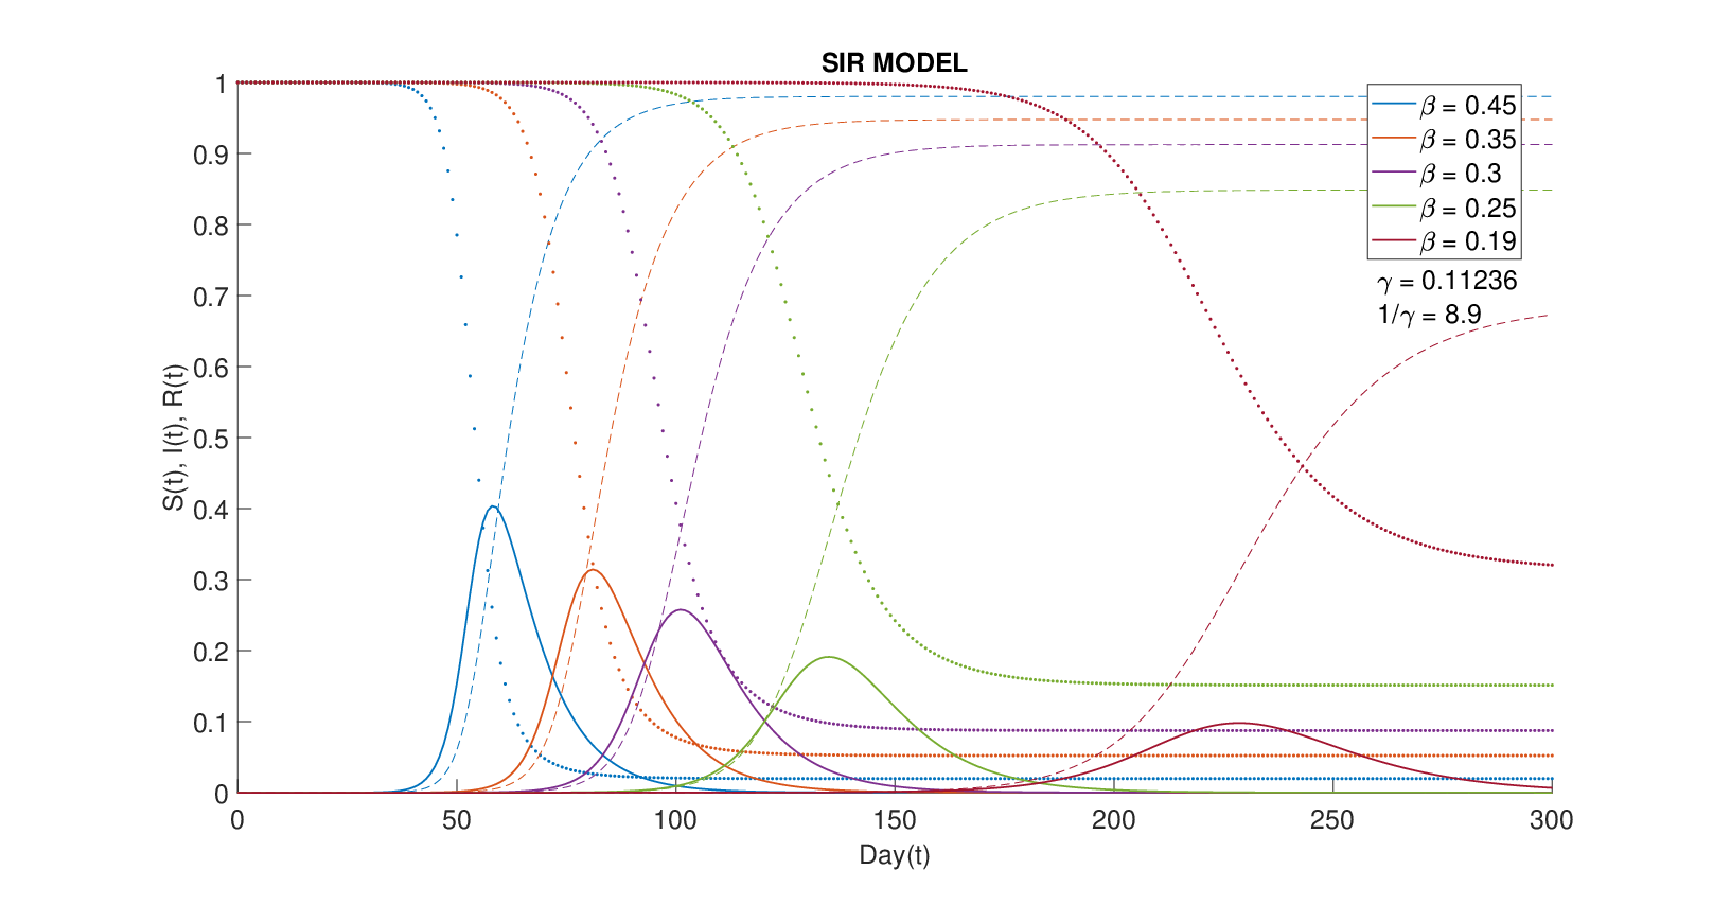
\includegraphics[width=0.48\linewidth]{0_introduction/images_introduction/sir_multipli_beta}} \\
	\caption[SIR dynamic example]{SIR system numerical solutions. Figure a) shows the evolution of compartments in the case of an epidemic. The violet dotted line represents the time-dependent $R_0(t)$. It can be seen that when this parameter is equal to $1$, the number of infected reaches its maximum value. In b) are presented different evolutions of the disease varying only the $\beta$ coefficient. The smaller its value the flattened and the more delayed the infectious curve is.}
	\label{fig:sir_example}
\end{figure}
Other two interesting quantities to consider when a new disease appears are the rate of increase of the infectious and the final size of remaining susceptible at the end of the epidemic. There is a large difference when a population suffers from an epidemic if this ends rapidly because a lot of people get sick or if this number can be controlled, and the infectious curve is flatter. A strategy to flatten the curve can reduce the contact between susceptibles, actuating social distancing or avoiding contact with infected, implementing quarantine measures. These are two simple examples of actions that reduce the value of $\beta$. Another countermeasure is represented by vaccination. Its immediate effect on the epidemic is to remove susceptibles people, so the disease can afflict only a small group and be quickly extinguished. 

\subsubsection{Stochastic models} 	
This is a group of models deriving by the mean-field, but using a different mathematical approach.
In this typology, the transition from one state to another is determined using a function of probability.  Conceptually are derived using the same framework used with ODE models. They are useful when the disease to study has a lower number of infected or if there is a connection between the epidemic outcome and changes in individual dynamics. This is called demographic variability, and it concerns changes in transmission, births, recovery, or deaths within the population. Using stochastic models with Monte Carlo simulations can be useful to investigate epidemic models on networks \cite{Allen2017}. 
The two most important types of models using this approach consider the time variable as continuous, $t \in [0, \infty) $and then the state variable is either discrete (Continuous-Time Markov-Chain) or continuous (Stochastic Differential Equations).
Referring to the SIR model to make a simple example here the S and I compartments are modeled as random variables. The probability of individuals changing groups depends on infection and recovery, the possible events that can occur. It is called transition probability. 
In a Markov chain approach the transition probability is discretized, and there is no dependence on the history of the epidemic to know how it will evolve at time $t + \Delta t$. It is necessary to know only the current state of the process at time $t$. 
In the Stochastic differential equation, the random variables are continuous. 

\subsection{Networked models}
\cite{Newman2002}, \cite{VanMieghem2009}, 


\subsection{Agent-based models}

VEDI E AGGIUNGI ANCHE \cite{Tizzoni2014}

Agent-based models are an alternative technique used to represent disease evolution. This approach is implemented based on the observation of spontaneous connections made by individuals. The evolution of a disease is considered over complex and realistic networks. The focus of this type of model is to understand how the network structure influences the epidemic by observing parameters such as the rate of spread.

In this framework, the nodes of the graph represent individuals (with all the properties that the modeler deems relevant for the study), while the edges represent interactions between people. Nodes can also represent subgroups of people, and using weights on edges makes it possible to characterize the strength of these interactions.

An advantage of this type of model is that it offers a very intuitive approach to epidemic modeling. Using an individual perspective guarantees an immediate interpretation of the model. A precise agent-based model can provide a greater understanding of the illness under consideration and direct information about countermeasures to implement to stop or mitigate its spread. However, to be powerful and capable of performing good analyses and predictions, a lot of information must be integrated into the model. Only if the agent-based model is highly capable of realistically reconstructing a real network can it be a reliable instrument, and achieving this requires very complex work.
\begin{figure}
	\centering
	\includegraphics[width=0.5\linewidth]{0_introduction/images_introduction/agent_based}
	\caption[Agent based network representation]{Agent based network representation}
	\label{fig:agentbased}
\end{figure}

%%

An example of a possible mathematical implementation of this class of models is now briefly presented. One possible technique to describe peer-to-peer contact in a graph structure is realized through a probabilistic framework. Here, assuming a total of $n$ agents in the model, spread processes can be described as a function of probability. Using Markov processes, each agent has a certain probability of transitioning from one state of the disease to another. To calculate the value of these probabilities, both the information derived from the network structure and parameters related to the disease, such as infectivity and recovery rates, are used. In this way, a stochastic evolution model of the processes is developed.

Considering an SIS model described with a Markov process: it has a dimension of $2^n$, while implementing an SIRS model requires a dimension of $3^n$. Because the size of models developed in this manner becomes rapidly enormous, a mean-field approximation is employed. It is based on the assumptions of a network composed of a sufficiently large number of agents and on the independence of these nodes. With this technique, by taking expectations, the transition rates of individuals are approximated. Using these approximations, the boundary values of the agent's probability of infection can be determined at each time step \cite{Hernandez_Vargas_2022}.

\subsection{Multilayer systems and networks} 

AGGIUNGI ANCHE \cite{Wang_2019}

The complex dynamic of interactions existing in the real world, develops in multiple patterns, with complicated relationships. This connection can change over time, and using the theory of multilayer systems it can improve the comprehension of such complexity. Additional information can be added to the model, for example, different types of interactions, like physical contact or information sharing, time dependency coefficients, or reliance between different parameters in nature, creating cause-effect relationships. 
It is a more recent development of the research, the traditional network theory was revisited, to create a framework that can include multiple networks, that evolve and influence each other \cite{DeDomenico2016} and can be helpful to manipulate complex systems like human relationships. Some interesting results obtained are the possibility that the onset of one disease can depend on the onset of the other one. There can be regimes in which the criticality of the two dynamics is interdependent and others in which the critical effect is only one-directional \cite{DeDomenico2016}. 
One possible way to develop models with this structure is to imagine that each layer represents a different type of interaction. An epidemiological example is a layer in which the physical contact between people is simulated and another represents social structure, the network of relations that every person has. This instrument provides a natural representation of coupled structure and dynamical processes. It has been presented in multiple works in the past years, for example in CITA. 
The dynamic realized in multiple systems can be single or coupled. In the first, there is a top layer with its dynamic evolution running on top of a multilayer network. The coupled structure instead is the one in which the phenomena described in each layer evolve with the influence of what is happening in the other. 
Multilayer networks have multiple dimensions of connectivity, called "aspects" and they have to be considered simultaneously. 
They can also be considered with two different mathematical structures. 
\begin{figure}[]
	\centering
	\includegraphics[width=0.6\linewidth]{0_introduction/images_introduction/multi_layer}
	\caption[Multi-layer network]{Representation of a multiplex structure. The figure is taken by the work of \cite{Granell2013} and shows the network implemented in their model. There is an awareness and an epidemic layer. In this case, the node connected with the interlayer connection represents the same individual.}
	\label{fig:multilayer}
\end{figure}

The first uses the same set of compartmental structure and mean-field models presented in the section before \ref{subsec:mean_field}. Here, from a mathematical point of view, there is no such difference in the manipulation and analysis of the system. The distinction relies on the meaning of the compartments and parameters created and on the dependence of the coefficients, which can be time and state-dependent.

The second option considers an agent-based structure. Here, considering a graph structure, composed of nodes and links between them, it is possible to classify three types of edges:
\begin{itemize}
	\item intra-layer edges, the connection of nodes on the same layer.
	\item inter-layer edges, the connection between a replica of the same node, but lying on a different layer of the structure;
	\item inter-layer edges, but coupling nodes representing distinct entities. 
\end{itemize}

A possible representation is done using a $4^{th}$ order tensor or coupling a set of adjacency matrices, called "supra-adjacency matrices". The feature that can be studied is the structural properties of the network, depending on how the various layers are coupled together. The presence of clusters or most central nodes is also important.

 
%%%%%%%%%%%%%%%%%%%%%%%%%%%%%%%%%%%%%%%%%%%%%%%%%%%%%%%%%%%%%%%%%%%%
\chapter{Review of epidemiological behavioural and opinion models in literature}
%NUOVO TESTO
The scientific community's interest in epi-behavior models has existed for several years. Initially, as noted by \cite{Bauch_2012_overview}, the behavioral aspect of epidemiology was not given significant attention. Its development has been a gradual process, resulting from years of evolution in research.

In fact, in the initial works \cite{kermack1927}, the focus of scientists was primarily on describing the evolution of diseases. The resulting models did not account for the effect of behavior; the population was considered homogeneously mixed, leading to random contact between susceptibles and infectives \cite{Hernandez_Vargas_2022, Mata2021}. 
It was only later, as epidemiological models proved effective and reliable in describing and predicting disease spread, that interest among policymakers grew. Tools capable of integrating real data with epidemiological models emerged, aiding decision-making on matters such as the duration of school closures or travel restrictions, as described in \cite{Bauch_2012_overview}.

Furthermore, new categories of models have emerged, such as agent-based models, networked models, and multi-layer/multi-system models. Despite their differing approaches, these models aim to integrate various population characteristics—such as contact structure, age distribution, and movement patterns—to address the limitations of the original homogeneity assumption \cite{brauer2012mathematical}.
This focus on societal composition and behavior naturally stems from the desire to use modeling tools as a reference for decision-making in safety and health. 
One possible approach to incorporating changes in the structure of models that describe aspects of behavior or population composition is to do so implicitly.

In these models, the behavior of the population is implicitly considered by integrating time-variable parameters that capture changes in societal behavior. This approach represents the classical modeling technique used in the formulation of epidemiological models. Examples of studies that have utilized this methodology for analyzing COVID-19 include \cite{Giordano_2020, Dehning_2020, Proverbio_2021}.

Although models developed in this way have proven to be powerful tools for generating insights about disease dynamics and providing recommendations to policymakers, they fall short in their ability to accurately reconstruct how populations behave during an epidemic outbreak. The desire to explore this aspect and develop a framework capable of simultaneously simulating both behavior and disease diffusion—where each mutually influences the other—has driven the development of a specific research field dedicated to behavioral epidemics.

But how can behavior be integrated into pre-existing epidemiological theory? To better address this question, we follow the classification proposed in \cite{Funk_2010}, which offers a possible subdivision of behavioral literature based on the different approaches that most articles focus on. Three major categories emerge:
\begin{itemize}
	\item The source of information used to make decisions;
	\item The type of information used to make decisions;
	\item The effect of behavioral change on the dynamic described by  the model. 
\end{itemize}
When analyzing the source of information, there is a clear distinction between works that assume governments and populations base their decisions on precise data, such as the number of infected individuals (prevalence), and those that consider more informal sources, such as conversations between people, public opinion, or media representations of the situation \cite{Bulai2023}. These media sources include both traditional outlets like television and newspapers, as well as newer platforms like social networks.
This distinction highlights the diversity in how behavioral factors are integrated into models, reflecting the varying degrees of reliability and influence these sources have on decision-making processes during an epidemic.


Regarding information quality and the negative effect of misinformation spreading within the population, an example is the fear of vaccination \cite{Kahan_2013}. Several works analyze the effect that fear of vaccination has had on the spread of infection \cite{Bauch_2012_game, Epstein_2021}.
An example of how this phenomenon can arise is the story of an article originally published by a prestigious source. Even though the thesis presented in this work was later proven wrong by the scientific community \cite{wakefield1998retracted}, the negative impact in terms of spreading fear about vaccines has persisted and, in many cases, has become deeply ingrained. In this specific case, it caused a decrease in herd immunity and a resurgence of measles \cite{Bauch_2012_overview}.


After introducing the impact that information quality may have, another interesting aspect is related to the different types of information used in model development. Some articles focus on the effect of media on behavior \cite{Collinson2014, Misra_2011}, while others consider peer-to-peer conversations, information exchange, and beliefs among individuals \cite{Tyson_2020}. These are completely different approaches, even though they aim to achieve the same effect: simulating the evolution of people's opinions and behavior. Using media involves hypothesizing that the population is influenced by a few "central" information nodes, so the same news, data, or future predictions are shared with everyone. In contrast, models that use personal information exchanges can depict a scenario where many different ideas about the disease situation circulate simultaneously.
Another concept used in models that simulate a sort of "collective consciousness" is referred to as "awareness" \cite{Funk2009}. To model how awareness spreads in the population, it is often treated like a disease \cite{Silva2019, Granell_2013, Granell2014, Kabir_2019, Zuo_2021, Wang_2019}. Although there are differences, the main idea is that theories and concepts about a certain topic can spread among people, which can be considered at a higher level as a unified opinion. For example, there may be many different personal positions on how to respond to a health emergency like COVID-19, but it is possible to abstract the various opinions and reconstruct what the majority of people, or macro-groups, ultimately feel. They may either be more cooperative and in favor of following guidelines issued by authorities or more focused on their well-being and inclined to act independently.
This process can be related to opinion formation studies, which aim to understand how people form their ideas \cite{Devia_2023, Devia2022} and also analyze the possible formation of opinion distributions, such as perfect consensus, consensus, polarization, clustering, or dissensus.

\chapter{Main objectives and thesis structure}

In this chapter, we present the main objectives of the thesis and describe its structure. Starting from an analysis of the theoretical contributions already developed for epidemiology, and in particular focusing on multilayer systems and mean-field models, the following questions are studied:

\begin{itemize}
	\item How can population behaviors be effectively included in epidemiological models? What are the characteristics that must be considered?
	\item Can individual behavior influence the evolution of an epidemic?
	\item Can an outbreak be stopped just  by relying on the natural subdivision of the population into compliant and non-compliant groups regarding safety measures, or is the intervention of a central "controller" necessary to enforce new behavior rules?
%	\item Is it useful for the model to create a quantity that express awareness of the society about the disease state? 
\end{itemize}
%About the last question, consciousness or awareness is a parameter considered useful to gain insight into society's reaction to the disease. Furthermore, there can be differences in behavior when the same conditions occur at different times, such as at the beginning of an outbreak versus several months later. For this reason, it is imagined a parameter that can change its value according to such dynamic and then it is tested how effectively is in the model. 

The quantity and quality of information available to the population can make a difference in how people deal with difficult situations.

Starting from these questions, the following objectives have been identified:
\begin{itemize}
	\item Create an original epidemic-behavioral multi-system model that captures the evolution of a disease and represents behavioral changes using a peer pressure mechanism within the same population.
	\item Add a control mechanism within the model, represented by government rules that can modify individual behaviors in a centralized way.
	\item Develop a comprehensive analysis of the epidemiological and behavioral model to understand its mechanisms and correctly interpret the mutual effects arising from the coupling of the social and epidemic phenomena.
	%\item Conduct a study using available data on population behavior during the COVID-19 pandemic to verify if the developed model can accurately reconstruct events and how people reacted to them.
\end{itemize}
The thesis is structured as follows. The introductory Chapter \ref{ch:theo_back} presents the main concepts of social science and epidemiology and provides all the necessary information to understand the presented research, including a glossary of the most important terms and an overview of the mathematical tools used in epidemiology. Additionally,  different models implemented to simulate an epidemic are shown in Section \ref{sec:models_categ}, with a focus on the properties of mean fields model, used in the thesis. Furthermore, a historical background of the research field is provided to give a perspective on the principal milestones.

Chapter \ref{ch:literature_review} offers a review of the literature analyzed for the thesis. The articles are categorized into different main topics: epidemiology theories, opinion models, behavior models, and multi-agent and multi-system models. This subdivision highlights the most interesting aspects of each work and identifies the elements that have been considered for inclusion in the thesis.

The second part of the thesis is composed of four main chapters. In chapter \ref{ch:why_new} the reasons that led to the development of a new model are presented.
In Chapter \ref{ch:model_alone}, the developed epidemiological and behavioral models are simulated. The SIRS epidemic model is presented, and its features are described. Conversely, the behavioral model developed for the thesis is introduced, the assumptions made for its dynamics are explained, and a set of simulations and analyses is performed. This analysis is conducted to gain a clear understanding of how the hypothesized social dynamics can evolve and to develop initial insights crucial for understanding the behavior of the fully coupled final model.
Chapter \ref{ch:epi_behav_model} presents the model resulting from the integration of the two layers, forming part of a more complex multi-system model. The implementation of this coupling is explained, detailing how the mutual influence between the two components operates. The main features of this model are analyzed using both simulations and insights gained from calculating the epidemic reproduction number. In fact, the threshold effect, which explains whether a disease-free equilibrium can evolve into an epidemic, is determined, and its value is calculated under varying model scenarios.
Finally the last chapter contains the conclusions of the thesis. 
\chapter{Theoretical background}
\label{ch:theo_back}
\section{Epidemiological theory: foundations}

A clear description of the main concepts in social science and epidemiology is essential for understanding the rest of the work. In this chapter, the theoretical basis and main concepts that will be used in the present work are defined. 

First, a brief historical review of the emergence of epidemiology as a discipline is provided, focusing on the explanation of its genesis. Indeed, these key findings laid the foundation of modern  epidemiology. 
The following section presents a glossary of the key terms used throughout this thesis to ensure clear communication of the core concepts that will be used later. Initially, terms related to epidemiology are explained, followed by definitions of behavior-related concepts.

Subsequently, the most commonly used mathematical tools are introduced, including an overview of various modeling techniques. Special attention is given to the theoretical background of mean-field models, the category to which the model developed in the thesis belongs.

\subsection{Epidemiological research: historical background}
\label{subsec:history}
% Se ti piace l'idea di fare un piccolo excursus storico, va bene. Le info principali sono:
% 1- primo lavoro di Bernoulli
% 2- lavori di Hamer (1906) mass action principle, epidemic description in discrete time 
% 3- Ross, formulation in continous time 
% 4- Kermack and Mc Kendrick (1927) che danno risultato bello perchè introducono "legge" del thresold di una epidemia
% Dopo aver scritto quest'ultimo evento hai il LA per parlare di come funziona un mean field model. 

The research field regarding the development of techniques to understand how epidemics can evolve over time has a history dating back to the 20th century. The first important discovery in this field must be attributed to the scientists that found the mechanism used by diseases to spread. 
A first innovative work was the one by John Snow, who during an epidemic of Cholera in London in 1854 successfully determined the source of the infection, even without knowing its etiological agent. Further advances in the microbiological research were due to Pasteur and Koch. They found the etiological agent of disease, enabling the possibility to treat and prevent people from being infected. Then, Hamer's work in 1906 added a first major theoretical contribution. He formulated a theory about the correlation between the course of an epidemic and the interaction, or contact ratio, between susceptible and infectious individuals. It was the so called “mass action” principle. The number of contacts between these two groups determines the spread rate of the disease. 
This law, originally written in discrete time, was then updated in 1908 by Ross, who wrote it  in continuous time. For the first time the problem could be studied using a clearly, well defined mathematical theory. Then the contributions of Kermack and McKendrick in 1927 added another fundamental principle to the modern epidemiology. They formulated a threshold theory explaining which conditions can generate the development of an epidemic. Their theorem states that a certain value -called reproduction number- must be exceed, depending on the proportion of susceptible and infectious individual. Monitoring this value allows us to understand if the number of infections will increase, until a peak is reached, or if the epidemic is in a descendent phase \cite{Mata2021, Anderson_82}. 
Their contribution based on the mass action principle represents the fundation for the mean field model theory, presented and analyzed in Section \ref{subsec:SIR}. 


\subsection{Epidemiological glossary}
\label{subsec:glossary}
For a better comprehension of the subject analyzed in the present work, a list of principal concepts and terms is presented. 

\subsubsection{CFR, IFR and mortality excess} The case fatality rate, CFR, is the ratio between the number of deaths due to a specific disease and the total number of confirmed positive cases detected by testing. 
The infection fatality rate, IFR, is instead the percentage of people infected with the disease that are expected to die. The two quantities can have a similar value: if every person who contracts the disease and every death attributable to the disease is known and recorded, then the CFR will equal the IFR.
The excess in mortality can be calculated by observing the difference between the total death rate (due to any reason) before and during an epidemic and one without. 


\subsubsection{Disease transmission} A disease can spread in different ways: 
	\begin{itemize}
		\item Person to person: involving direct (e.g. sexual transmission or skin diseases) or indirect (e.g. respiratory) contact.
		\item Airborne: through inhalation of infected air.
		\item Food or water borne: ingesting contaminated food or water. 
		\item Vector born: the contagion is mediated by infected animals.
	\end{itemize}
	Furthermore, when the spread is within the same generation the transmission is called horizontal, while vertical transmission is the one between different generations, from parents to children. 
	Zoonosis is the phenomenon in which a disease that starts in an animal species mutates and infects humans. The opposite can also happen and it is called inverse-zoonosis. 

\subsubsection{Endemic disease} It is a disease that lasts for a long time and requires consideration of its impact on population renewal and in the number of susceptible individuals.
	
\subsubsection{Epidemic disease} An increase in disease prevalence typically manifests as a rapid outbreak. This type of illness is confined to a limited geographical region, unlike a pandemic that affects a much larger area.

\subsubsection{Immunity and herd immunity}
Immunity refers to the protection from a disease gained after contracting it (or after the vaccination). This immunity can be lifelong or diminish over time. When a person is immune, re-exposure to the virus does not result in infection, or there is only a reduced chance of being infected, known as partial immunity.

Herd immunity is a phenomenon where a large portion of the population becomes immune, either through vaccination or surviving the disease. This majority limits the spread of the illness, indirectly protecting those who are not immune by slowing or halting disease transmission.

\subsubsection{Incidence and prevalence} The first term refers to the number of new cases within a certain period (daily or weekly for example), while prevalence is the portion of the population affected by a disease in a specific time.

\subsubsection{Incubation, Symptoms, Infected and Infectious}  When a person comes into contact with an infectious individual, they may or may not become infected. The incubation period refers to the time after infection when the disease grows within the host without producing symptoms.

Symptoms refer to the physical signs of illness caused by a disease in the affected individual.

A person is described as infectious when they carry the disease and can transmit it to others, while infected refers to someone who has been exposed to the infection and has become ill.

\subsubsection{Incubation period and serial interval} The incubation is the time after exposure in which the infection develops in the host and ends when the infected start to show symptoms. The serial interval is instead the time that exists between two transmissions in a chain of infections. 


\subsubsection{Micro and Macro parasite}
An etiological organism responsible for a disease can be either a  microparasite or a macroparasite. The former lives and reproduces within the host, generating an immune response and causing an infection that usually has two possible outcomes: death or immunity. Infections due to microparasites are shorter than the life span of an individual, and have a transient nature. Most viral and bacterial parasites belongs to the microparasitic category.

Instead, macroparasites have no direct reproduction within their host. Arthropods and helmints are in this category. They are larger and have a much longer generation times than microparasites, with a life span that can be a considerable fraction of the host life span.


\subsubsection{Outbreak} The rapid raise in the number of infected during an epidemic.


\subsubsection{Overdispersion and Superspreading} Overdispersion is a term that refers to observing a larger variance than expected from a normal distribution. It is used in statistics to measure superspreading, a circumstance in which there is an abnormal (higher) number of secondary infections brought about by low numbers of spreaders.

\subsubsection{Pandemic disease} It is an epidemic that spreads across multiple regions, on a global scale. The severity of the disease also makes a distinction in calling a disease a pandemic. For example, the common cold is spread in the whole world but is not defined as a pandemic by the WHO (World Health Organization). 

\subsubsection{Reproduction number $\mathcal{R}_0$} It is the fundamental measure of the infectiousness of a disease. It is the average number of secondary infections caused by one infected person in a fully susceptible population. If it is recalculated during the epidemic progression it is called $\mathcal{R}(t)$, a time-varying reproduction number, also called the effective reproduction number: it is obtained by rescaling the Reproduction number value with the true number of susceptible individuals.

\subsubsection{Types of infectious diseases}An infectious disease is an illness resulting from the presence of pathogenic microbial agents such as bacteria, viruses, parasites or other microorganisms.

It is possible to distinguish between \textit{transmittable} and \textit{communicable} disease. A transmittable disease can be transmitted between persons through close contact (e.g. blood borne transmitted sexually or through bodily fluids). A communicable disease is one that easily spreads from one person or animal to another by casual contact or from a surface to a person.  


\subsubsection{Virulence and Contagiousness}  Virulence is used to describe how aggressive, harmful, and pathogenic is a biological agent in attacking cells. Contagiousness is the capability to transmit a disease. 


%%%%%%%%%%%%%%%%%%%%
\section{Opinion/behaviour glossary}
To establish a framework suitable for developing and understanding behavioral models, the following key concepts from social science are outlined.
\subsubsection{Awareness} It is the knowledge and alert level that an individual has on a certain subject or situation. It changes with time and it is developed with information or experience.  

\subsubsection{Behaviour} It is how one acts or conducts oneself. It can depend on the response to external stimuli and have effects, especially on others.


\subsubsection{Belief} It is the conviction of the truth of a statement or the reality of a being or phenomenon, especially when based on the examination of evidence, but also on matters for which there is no proof.


\subsubsection{Group decision-making} It is a phenomenon at the intersection of psychology, management, biology, and applied mathematics studying how people in groups interact, exchange information, and realize decisions. The decision made by the group is no longer attributable to any single individual but to the whole group. 

\subsubsection{Homophily} The tendency to bond and associate preferentially with similar others. 

\subsubsection{Information} The term "information" is commonly understood as "knowledge communicated." However, given its crucial role in modern society, there is considerable debate about its various meanings \cite{Capurro_2003}. Today’s world is often described as an "information society," where the advancement of information technology has impacted nearly every aspect of life.

Currently, the term "information" carries two key meanings. The first, more general, definition refers to anything that is valuable in answering a question. The second definition pertains to Information Science, the discipline that manages information in all its forms. In this context, information is something with the capacity to inform. On a fundamental level, anything that is not entirely random can be considered to convey some degree of information. 

\subsubsection{Perception} It is the mechanism through which something is regarded, understood, or interpreted.

\subsubsection{Polarization and Consensus}

Polarization refers to the divergence of beliefs within a population. There are several mathematical methods available to measure the degree of polarization. For instance, one can collect data on opinions, beliefs, or behaviors within a group and then measure the distance between the most extreme views, or analyze their distribution across a defined range.

This contrasts with the concept of "consensus," where the exchange of opinions, information, or resources among individuals leads to widespread agreement. Both polarization and consensus can be studied and modeled using network theory \cite{Devia2022}.
\subsubsection{Threshold theory}
It is a theory formulated by Granovetter in \cite{Granovetter_1978} regarding collective behavior. The theory posits that in a society where individuals face two possible alternatives, and their choices involve certain costs and benefits depending on how many others choose each alternative, an individual will decide based on the number of others who have already chosen a particular option when this number exceeds a certain threshold.

\subsubsection{Trust} It is the sentiment of confidence associated with the ability, strength, and truth of someone or something. 

\section{Epidemiological models categorization}
\label{sec:models_categ}
Starting from the observation of the real world, the desire to better understand a certain phenomenon is the fundation of mathematical model development. A perfect model does not exist, because each model is based on data or on assumptions that are incomplete with respect to reality. However, a useful model allows us to provide general predictions and can be a powerful instrument for researchers and policymakers. For example, an application is the estimation of the effects of certain policies on the population during an epidemic: in this case, the aim is to obtain meaningful prediction, under a given set of real-world circumstances.
When working on a model, the importance of the uncertainty related to the obtained predictions and forecasts must always be remembered. This concept is remarked also in the definition of mathematical model present in \cite{Ledder_2023}. 
\begin{displayquote}
	"A Mathematical model is a self-contained collection of one or more variables together with a set of rules (usually formulas and equations) that prescribe the values of those variables. Models serve as an approximate quantitative description of some actual or hypothetical real-world scenario. They are created in the hope that the behavior they predict will capture enough of the features of that scenario to be useful."
\end{displayquote}

There are several different types of mathematical models.
A first classification can be done considering the method used to obtain them: we thus have mechanistic, empirical, phenomenological or conceptual models.
Mechanistic models are based on assumptions about reality, or theoretical principles, modeled using a collection of one or more variables together with a self-contained set of rules. These models have an explanatory value on the reality they represent.
Empirical models are realized by fitting set of data. They are a powerful instrument, because data can be fitted quite well, but they lack the explanatory value of mechanistic models.
A phenomenological model describes the empirical relationships between phenomena in a way that aligns with fundamental theory, but it is not directly derived from first principles. These models define the relationships between variables and provide insights into the phenomenon under study. 
%They are particularly useful in cases where no exact analytical solution exists to explain a certain scientific phenomenon.
Finally, a conceptual model is a verbal description of a real-world phenomenon. 

In the thesis, we consider mechanistic/phenomenological models. In fact, in epidemiology, the objectives for which a model is developed go beyond just fitting data. Examples of possible objectives are:
\begin{itemize}
	\item monitor the epidemic evolution;
	\item realize a framework capable of understanding the information related to the disease, as incidence and prevalence for example;
	\item obtain general insight about epidemic control strategies;
	\item realize predictions.
\end{itemize}
Several different types of mechanistic models have been developed or are adapted to be used in epidemiology modeling. In this section, the principal typologies are now introduced. 

In particular, mean-field models are discussed in depth in section \ref{subsec:SIR}, because the multi-system model developed in the thesis belongs to this class.

%A focus on mean field model and its basic theoretical concepts is presented in section \ref{subsec:SIR}, because it represents the mathematical base model of the multi-layer system implemented in the present work. 

We introduce the logic underlying their structure, their main mechanisms, and the important conclusions that can be derived from them because it is a useful introduction to the approach that will later be employed in the rest of the thesis.

\subsection{Mean field models}
\label{subsec:mean_field}
 Mean field model, also known as compartmental model, is the first developed and most studied type of mathematical model used in epidemiology \cite{kermack1927, brauer2012mathematical, Anderson_82, anderson1991infectious}. A mean field model assumes that a well-mixed population is divided into several subgroups (i.e. compartments). Each compartment is associated with a different stage of the disease under consideration. Some possible states are susceptibles, asymptomatic (infected), symptomatic (infected), infected (if in the model no distinction between symptomatic or asymptomatic is done), exposed, vaccinated, quarantined, dead, recovered, and hospitalized. The classes considered in a given model determine its base structure. The choice to include a certain compartment depends on the disease that is modeled and on the considered assumptions. Different models can be suitable to analyze the same disease but can be used with different aims. A more complex model can emphasize some aspects or effects of the disease, that are not highlighted by a simpler one.
 
For example, both a SIR (Susceptible- Infectious-Recovered) \cite{Dehning_2020} and a SPQEIR (Susceptible -Protected-Quarantined- Exposed- Infectious- Removed) \cite{Proverbio_2021} can be used to model COVID-19, but the second model considers explicitly quarantine, exposed and use of protections to avoid infection - elements that cannot be observed or considered with a simpler model like a SIR.
  
In mean-field class of models, the primary focus is to describe the spread of the disease rather than its biological impact on the health of each infected individual. The transitions between compartments (such as Susceptible, Infected, and Recovered) are governed by differential equations. The parameters that control these transitions are coefficients whose interpretation depends on the underlying assumptions of the model. For example the $\gamma$ parameter is usually interpreted as the inverse of the time an individual spend in the infectious compartment. Mathematically, these parameters determine the rate of flow between compartments. 

The most critical metric in this model category is the "Basic Reproduction Number" (often denoted as $R_0$), which represents the average number of secondary infections caused by a single infected individual in a fully susceptible population. It is a fundamental threshold in epidemiology, indicating the potential severity of an outbreak \cite{Hernandez_Vargas_2022}. By observing the value of $R_0$, it is possible to immediately determine whether a newly developed disease can spread within the susceptible population and cause an outbreak leading to an epidemic.
\begin{figure}[]
	\centering
	\includegraphics[width=0.65\linewidth]{0_introduction/images_introduction/SIRS_figure_compartmental}
	\caption[SIRS example]{An example of the graph structure of a mean field SIRS model. There are three compartments and the flow rate between them is ruled by the coefficients $\beta$ (transmission rate), $\gamma$ (recovery rate) and $\delta$ (immunity waning rate).}
	\label{fig:sirsfigurecompartmental}
\end{figure}


\subsubsection{SIR model}
\label{subsec:SIR}
The foundational model for studying epidemics mathematically is the SI model. In this model, the population is divided into two compartments: Susceptible $(S)$ and Infected $(I)$. Individuals transition from being susceptible to infected, but there is no recovery, meaning once infected, individuals remain infectious indefinitely.

T SIR model adds a third compartment, Recovered or Removed $(R)$. This additional compartment represents individuals who have either gained immunity or have died, and are thus removed them from the cycle of infection. After spending a certain period in the infected state, individuals transition to the recovered state, making them no longer susceptible to the disease.
Now to begin introduce the SIR model structure, first its compartments subdivision is presented. The population or density of individuals is sub-divided into three groups: Susceptible, Infectious, and Recovered. At time $t$ the three groups are identified with the symbols: $S(t)$, $I(t)$, and $R(t)$. 
The symbols used to indicate the fractions of population in each group are instead $s$, $i$, and $r$, while the capital letters are used to specify both the name of the groups or the absolute number of individuals in each one. 

The SIR model, which will be described in the following sections, is built upon several assumptions that shape the mathematical framework. These guiding principles are introduced in the following paragraphs. Furthermore, the main properties of the model will also be introduced. 

\subsubsection{Mean-field approximation}
The approximation that gives the name to this model class is based on a method that permits the analytical analysis of complex systems. With mean-field, individual-level interactions are averaged, focusing not on individual behavior but on the collective behavior of the population. Using this method, equations can be derived that describe disease evolution in terms of average rates rather than tracking individual agents.
\subsubsection{Homogeneus mixing} 
It is the assumption that all individuals in the population mix homogeneously, meaning that the probability of interacting with any individual is the same. It is a strong assumption because it implies ignoring any spatial or social structure.
\subsection{Average rates of changes}
\label{sec:sir_presentation}
In the model, differential equations are used to represent the transition of individuals between different compartments. These transitions can depend on the state of the system but, in the simplest form, are based on average rates. The three rates used in the SIRS mean-field model are:
\begin{itemize}
	\item $\beta$: transmission rate;
	\item $\gamma$: recovery rate;
	\item $\delta$: waning immunity rate.
\end{itemize}
The flow of individuals in the system is shown in Figure \ref{fig:sirsfigurecompartmental}.

\subsubsection{Population conservation}
The total population size, represented by the letter $N$, is the sum of the numbers of individuals in the compartments (e.g., Susceptible, Infected, and Recovered). It is often assumed to remain constant during the course of an epidemic. This assumption is based on the idea that epidemics typically last much shorter than the average human lifespan, making the effects of births and deaths negligible.
In more complex models, where demographic effects are considered, such as in models of longer-lasting epidemics, the population size can still be assumed constant by balancing the number of births (modeled as an influx into the Susceptible compartment) with the number of deaths (modeled as an outflux). This approach assumes that births and deaths occur at approximately the same rate, keeping the total population size constant over time. The result of this assumption implies that:
\begin{itemize}
	\item The population densities in the compartments sum up to one.
\end{itemize}
\[s(t) + i(t) + r(t)= 1 \]
\begin{itemize}
	\item The sum of their time derivatives is equal to zero.
\end{itemize}
 \[\dot{s}(t)+ \dot{i}(t) + \dot{r}(t)= 0\]

\subsubsection{Recover transition} 
The first fundamental dynamic process of the model assumes that the infected compartment decreases in size with a rate of decrease proportional solely to the current number of infected individuals. This gives the following relation:
\[\frac{d i}{dt} = - \gamma i, \qquad i(0) = i_0, \]
which models a continuous process. Specifically, it assumes that individuals transition from the infectious state to the recovered state at a constant rate, denoted by $\gamma$. The physiological meaning of this parameter is that it represents the inverse of the infection duration, i.e. that the average infection lasts $1/\gamma$ days. Thus, $\gamma$ is the recovery rate, reflecting the speed at which the population recovers from the disease.
 
%In this model the disease reproduces through horizontal incidence, and so the contagion is modeled as due to random contact that happens in a homogeneosuly mixed population.
\subsubsection{Person-to-person disease transmission}
\label{subsubsec:p2p_transmission}
Assuming a population composed of susceptible and infected individuals, each infectious individual encounters a fraction $c$ of the population per day. If all encounters are equally likely, a fraction $s$ of these encounters will be with susceptibles. Therefore, each infectious individual has $c\cdot s$ encounters with susceptibles. The probability that an encounter leads to transmission is $p$, hence the average number of transmissions per day is $p \cdot c \cdot s$. Considering the fraction of infected individuals $i$, and combining $p$ and $c$ into a single parameter $\beta$, the transmission rate becomes:
\[\text{transmission rate} = \beta s i.\]
Here, $\beta$ represents the transmission coefficient.


\subsubsection{Immunity}
In SIR model, once individuals recover from the disease, there are no further transitions. Two possible model scenarios can cause this:
\begin{itemize}
	\item Lifelong immunity acquired after recovery.
	\item Death of infected individuals.
\end{itemize}
Both cases assume that, once the illness period ends, the disease can no longer be transmitted.
If immunity acquired from an infection wanes after a certain period, individuals can become susceptible again, leading to an SIRS model. The $\delta$ rate is used to express the outflow from the Recovered compartment, and it corresponds to the inverse of the average duration of immunity.

\subsubsection{Threshold value}
\label{subsub:threshold}
Although the SIR model is simple, it plays a fundamental role in predicting a key aspect of epidemics: the threshold value, a concept first introduced by Kermack and McKendrick in their pioneering work \cite{kermack1927}. They showed that, in a fully susceptible population, an epidemic will only start if the basic reproduction number $\mathcal{R}_0$ is greater than $1$, marking the birth of the term "threshold value" in epidemiology.
In the SIR model the reproduction number value is equal to the ratio between the transmission and recovery rate:
\begin{equation}
	\mathcal{R}_0 = \frac{\beta}{\gamma}. 
	\label{eq_basic_reproduction_number}
\end{equation}

Over the years, the dynamics of this system have been extensively studied and analyzed \cite{Breda_2012, akinboro2014numerical, Jard_n_Kojakhmetov_2021, Ledder_2023, Okabe_2020, Prodanov_2022, Xu_2014, Turkyilmazoglu_2021}. The threshold effect highlights two distinct scenarios:
\begin{itemize}
	\item \textbf{Free Disease Equilibrium $(\mathcal{R}_0 < 1)$:} When $\mathcal{R}_0$ is less than one, the disease does not spread within the population. Although infected individuals make contact with susceptibles, the rate of disease transmission is slower than the recovery rate. Mathematically, this means $\beta / \gamma < 1$, or $\beta < \gamma$, where $\beta$ represents the transmission rate and $\gamma$ the recovery rate. Consequently, the healing process is faster than the spread of infection, and the number of infected individuals quickly drops to zero. The majority of the population remains susceptible, and the Disease Free Equilibrium is globally asymptotically stable, as demonstrated by \cite{Hernandez_Vargas_2022}.
	\item \textbf{Epidemic spread $(\mathcal{R}_0 > 1)$:}     When the threshold is greater than one, the number of infected individuals grows until it reaches a peak and then declines toward zero. The peak number of infected people, as well as the final number of susceptibles, can be calculated using the system initial conditions and the values of $\beta$ and $\gamma$, as described by \cite{Hethcote_2000}. 
	As reported in this work:
	\begin{quotation}\small
	Let $s_s(t),i_s(t)$ be a solution of the system 
	\begin{equation}
		\begin{split} 
			ds/dt &= -\beta i s\\
			di/dt &= \beta i s - \gamma i	
		\end{split}
	\end{equation}

	with $s(0) = s_0 \ge 0$, and $i(0) \ge 0$. The mass conservation assumption holds so $r(t) = 1-s(t)-i(t)$. The triangle in the $si$ phase plane given by 
	\[T ) {(s,i)|s \ge 0, i\ge 0, s+i \le 1 }\]
	is positively invariant and unique solutions exist in $T$ for all positive time, so that the
	model is mathematically and epidemiologically well posed.
	If parameter $\sigma$ is defined as $\sigma=\beta/\gamma$ it holds that if $\sigma s_0 >1$, the $i(t)$ first increase up to a maximum value $i_{max} = i_0 + s_0 - 1/\sigma - [\log(s_\infty/s_0)]/\sigma $ and then decrease to zero as $t \rightarrow \infty$. The susceptible fraction $s(t)$ is a decreasing function and the limiting value $s_\infty$ is the
	unique root in $(0, 1/\sigma)$ of the equation
	\[
	i_0 + s_0 -s_\infty - \log(s_\infty/s_0)/\sigma = 0. 
	\]		
	\end{quotation}
	
	This scenario illustrates how a highly aggressive infection can spread widely within a population. If no countermeasures are taken, it can lead to significant social and economic consequences. A typical epidemic outbreak has an infective curve that first increases from an initial Io near zero, reaches a peak, and then
	decreases toward zero as a function of time. The susceptible fraction $s(t)$ instead always
	decreases, but the final susceptible fraction $s_\infty$ is positive. The epidemic dies out because, when the susceptible fraction $s(t)$ goes below $1/\sigma$, the replacement number $\sigma s(t)$ goes below 1.
		
\end{itemize}
	Thus, even with its simplicity, the SIR model provides critical insights into the potential severity of an epidemic and highlights the importance of timely interventions to prevent widespread harm.
	

\subsubsection{The SIR mean-field model equations}
After introducing the basic framework of the model, the set of differential equations that describe the rates of change in the system states is presented. The equations, along with initial conditions, are necessary to fully define the model. The class sizes are expressed as fractions of the total, constant population.

The model is then
\begin{equation}
	\begin{cases}
		ds(t) / dt = -\beta s(t) i(t), \;\qquad \qquad s(0) = s_0 \gg 0;\\
		di(t) / dt =  \beta s(t) i(t) - \gamma i(t), \qquad i(0) = i_0 > 0;\\
		dr(t) / dt =  \gamma i(t), \qquad \; \, \;\quad \quad \qquad r(0) = r_0 = 0;
	\end{cases}
\end{equation}
where
\begin{equation}
s_0 + i_0 + r_0 = 1.
\end{equation}

Several works analyze this model and provide a detailed mathematical derivation of its solution \cite{diekmann2000mathematical,akinboro2014numerical,Turkyilmazoglu_2021}. However, this is not the focus of the present work. Instead, we provide an overview of the main results and a summary of the dynamics that emerge from the model.

\subsubsection{Model behavior}

To present the evolution of the model, a simple numerical simulation is carried out. The removal rate is set to $\gamma = 0.1$, meaning the infection lasts, on average, 10 days. The transmission rate is $\beta = 0.5$. At the start of the simulation, the majority of the population is in the susceptible class, with only a small portion of individuals already infected.

The initial reproduction number is  $\mathcal{R}_0 = 5$, which is greater than 1. As discussed in Section \ref{subsub:threshold}, this indicates that the disease will evolve into an epidemic.

The key features that emerge from the model simulation are:

\begin{itemize}
	\item \textbf{Slow initial phase:} The early stages of the epidemic are marked by a slow start, as seen in the first part of the curves in Figure \ref{fig:sir_example0}a. The curves remain nearly flat because only a few individuals are initially infected, and it takes time for the infection to spread and reach a larger portion of the population.
	\item \textbf{Exponential growth:} In the second stage, the number of infections increases exponentially.
	\item \textbf{Peak infection:} Eventually, the number of infections reaches a peak.
	\item \textbf{Residual susceptible population:} By the end of the epidemic, a portion of the population remains susceptible, though this amount depends on the model parameters.
\end{itemize}

An additional detail emerging from the model, as analyzed in \cite{Okabe_2020} and visible in Figure \ref{fig:sir_example0}, is the evolution of the reproductive ratio over time. The reproductive ratio is given by the formula $\mathcal{R}(t) = \frac{\beta}{\gamma} \cdot s(t)$. Initially, assuming $s(0)\approx 1$, we can simplify this to obtain the value of $\mathcal{R}_0$. However, as the susceptible fraction decreases exponentially alongside the growth in infections, the reproductive ratio also decreases, and the infection peak occurs when $\mathcal{R}(t)=1$.


\begin{figure}[ht]
	\centering
	\subfloat[][\emph{}]
	{\includegraphics[width=0.48\linewidth]{0_introduction/images_introduction/sir_con_rt}} \quad
	\subfloat[][\emph{}]
	{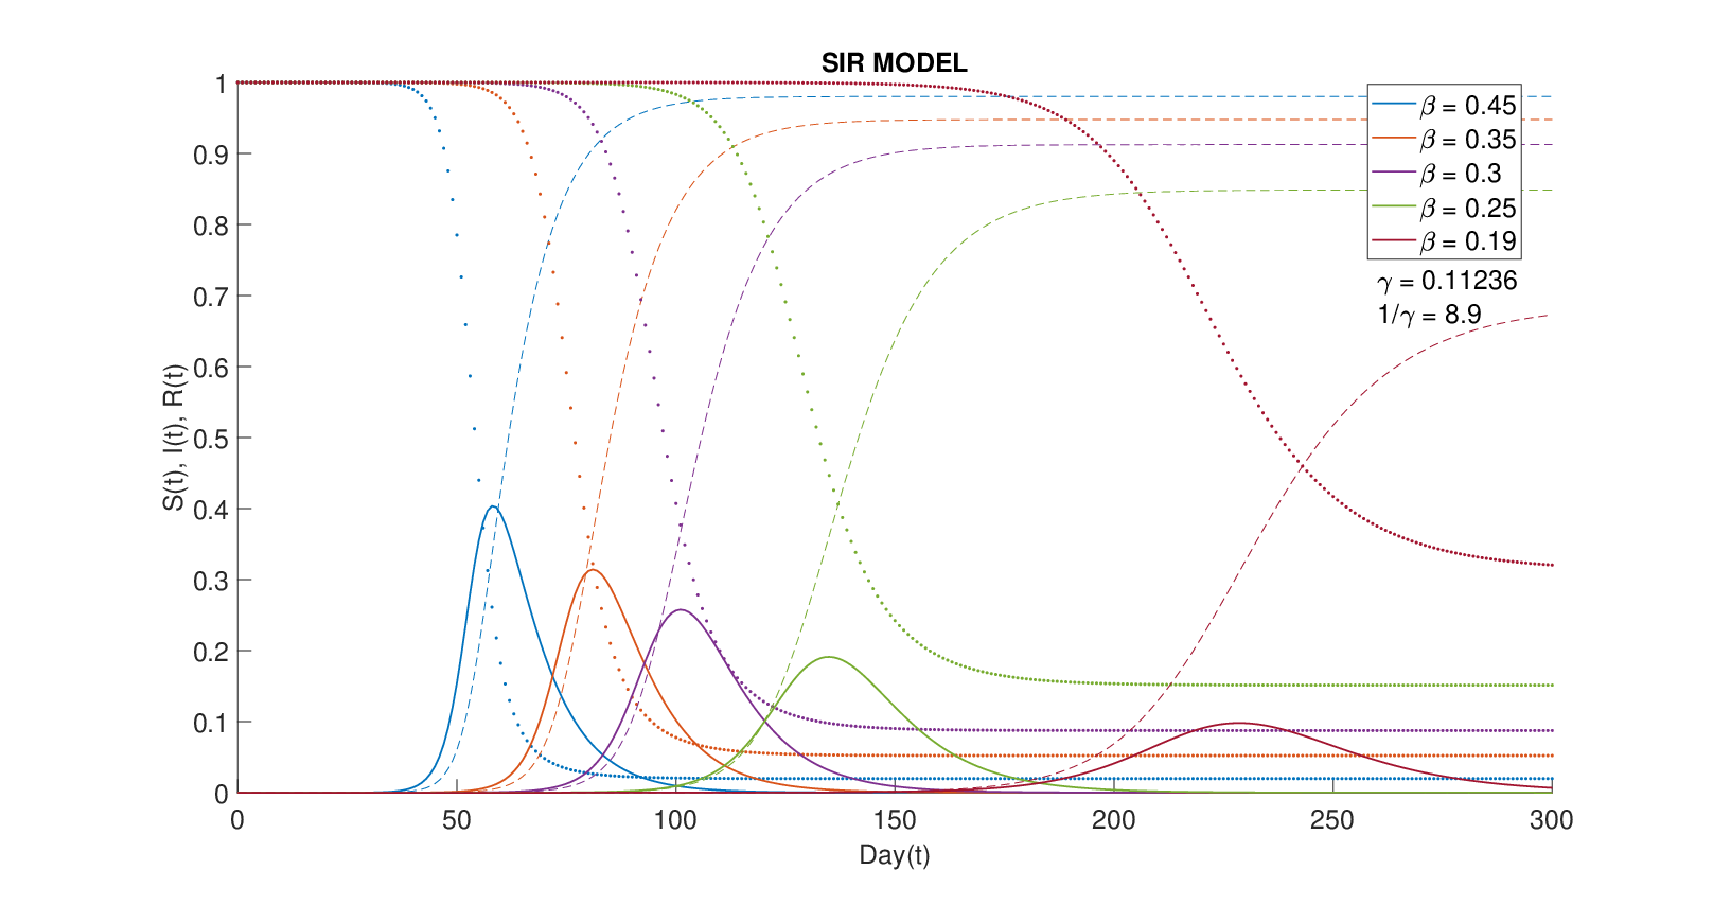
\includegraphics[width=0.48\linewidth]{0_introduction/images_introduction/sir_multipli_beta}} \\
	\caption[SIR dynamic example]{SIR system: numerical solutions. Panel a) shows the evolution of the model variables in the case of an epidemic. The violet line represents the time-dependent $\mathcal{R}_0(t)$. When this parameter is equal to $1$, the number of infected reaches its maximum value. Panel b) presents different evolutions of the disease obtained by varying only the $\beta$ coefficient. The smaller its value, the more flat and delayed the infectes curve is.}
	\label{fig:sir_example0}
\end{figure}
Two key metrics to consider during the emergence of a new disease are the rate of increase of infections and the final size of the remaining susceptible population by the end of the epidemic. The course an epidemic takes can vary dramatically depending on whether it spreads rapidly, overwhelming healthcare systems, or whether interventions succeed in "flattening the curve."
The rate of infection growth depends on how quickly the disease spreads through the population. If an epidemic grows rapidly, a large number of people fall ill in a short period, potentially overwhelming healthcare resources.
On the other hand, the final size of the susceptible population indicates how many individuals remain uninfected once the epidemic has run its course. This is influenced by factors such as herd immunity or interventions like vaccination.
"Flattening the curve" refers to strategies aimed at slowing the spread of the disease, thereby reducing the peak number of infections and spreading cases over a longer period. This reduces the strain on healthcare systems without necessarily reducing the total number of infections.

Some strategies for flattening the curve include:
\begin{itemize}
	\item Social distancing and quarantine to reduce contact between susceptible and infected individuals. This decreases the transmission rate $\beta$.
	\item Vaccination, which immediately reduces the number of susceptible individuals, thus preventing the disease from spreading widely.
\end{itemize}
While flattening the curve may not lower the total number of infections (i.e., the cumulative number may remain the same), it reduces the number of active cases at any given time, which is crucial for ensuring that healthcare systems are not overwhelmed.


\subsection{Other modeling techniques}
There are several other ways to model an epidemic, and the main types of models are now introduced. Many of the articles that will be reviewed in Chapter \ref{ch:literature_review} make use of one or more of these model types.
\subsubsection{Stochastic models} 	
This group of models, which originate from the mean-field approach, utilizes a different mathematical framework. In these models, the transition between states is governed by stochastic functions. Conceptually, they share the same foundation as ordinary differential equation (ODE) models but differ in application. These stochastic models are particularly useful when studying diseases with a lower number of infected individuals or when the epidemic outcome is influenced by changes in individual dynamics, a phenomenon known as demographic variability. Demographic variability includes changes in transmission rates, birth rates, recovery rates, or mortality within the population.
AN approach to model such variability is through stochastic models paired with Monte Carlo simulations \cite{Allen2017}.

\subsubsection{Networked models}
In this class of models, disease dynamics are considered over complex and realistic networks, with a focus on understanding how the network structure impacts the epidemic spread by analyzing parameters such as the rate of infection. The model represents individuals as nodes in a graph, with edges illustrating interactions between them. Nodes can also represent subgroups, and the relationships between individuals or groups can be weighted, representing varying strengths of interactions \cite{Newman2002,VanMieghem2009}. The larger the number of nodes and the more accurately the connections reflect real-world interactions, the better the model is at faithfully reproducing the spread of the disease.


\subsubsection{Agent-based models}
Agent-based models (ABMs) simulate the progression of a disease by focusing on the behavior and interaction of autonomous agents, which could be individuals or collective entities like organizations. This modeling approach is built on observing spontaneous interactions between individuals \cite{Tizzoni2014}, creating a dynamic system where each person acts according to certain rules. The goal is to understand how these individual behaviors influence the overall evolution of the system.

One key advantage of ABMs is that they provide an intuitive way to interpret epidemic modeling by focusing on individual perspectives, making the model results easier to understand. Additionally, because agents act according to individual behavior, ABMs can deliver highly detailed simulations and offer insights into specific countermeasures that might help mitigate the spread of a disease.

However, ABMs require a large amount of detailed, reliable data to be effective, as their accuracy depends on the precision of the information integrated into the model. Collecting and incorporating this data can be a challenging task, which is a potential limitation of this modeling approach \cite{Hernandez_Vargas_2022}.
\begin{figure}
	\centering
	\includegraphics[width=0.5\linewidth]{0_introduction/images_introduction/agent_based}
	\caption[Agent based network representation]{Agent based network representation.}
	\label{fig:agentbased}
\end{figure}

\subsubsection{Multilayer systems and networks: multi-system models} 
The complex dynamic of interactions existing in the real world, evolves in multiple patterns, with complicated relationships, that can change over time. Using the theory of multilayer systems can improve the comprehension of such complexity. Additional information can be added to the model, for example, different types of interactions, like physical contact or information sharing, time dependency coefficients, or reliance between different parameters in nature, creating cause-effect relationships.
\begin{figure}[ht]
	\centering
	\includegraphics[width=0.5\linewidth]{0_introduction/images_introduction/multi_layer}
	\caption[Multi-layer network]{Representation of a multilayer structure. The figure is taken from \cite{Granell2013} and shows a network implemented in their model. There are two layers coupled together: one representing awareness and the other the epidemic state. In this case, nodes connected by interlayer connections represent the same individual. Thus, the model describes people with two attributes: awareness of a disease and health state. The mechanisms of infection and becoming aware are distinct, but both attributes influence how an agent's state evolves. For example, if an agent is aware of the disease, they may act more cautiously, thereby reducing their probability of becoming infected.}
	\label{fig:multilayer}
\end{figure} 
Recent research developments revisits the traditional network theory to create a framework including multiple networks, that evolve and influence each other \cite{DeDomenico2016, Krickel_2023} and can be helpful to describe complex systems like human relationships. For instance, the onset of one disease may depend on the onset of another. There can be regimes in which the criticality of the two dynamics is interdependent and others in which the critical effect is only one-directional \cite{DeDomenico2016}. 
One possible way to develop models with this structure is to imagine that each layer represents a different type of interaction. For instance a model that considers, for each agent, both its physical contacts with others, where the disease can be transmitted, and its network of relations, representing the social dynamics in which everyone is involved. An example of this network is shown in Figure \ref{fig:multilayer}. This instrument provides a natural representation of coupled structure and dynamical processes. It has been used in multiple works in the past years, for example in \cite{Wang_2019}. 
Multiple systems can have either a single or coupled dynamic. In the case of a single dynamic, there is a top layer whose evolution occurs independently on top of a multilayer network. In contrast, a coupled structure describes phenomena in each layer evolving under the mutual influence of what is happening in the other layers.


%%%%%%%%%%%%%%%%%%%%%%%%%%%%%%%%%%%%%%%%%%%%%%%%%%%%%%%%%%%%%%%%%%%%

%
%%%%%%%%%%%%%%%%%%%%%%%%%%%%%%%%%%%%%%%%%%%%%%%%%%%%%%%%%%%%%%%%%%%%
\chapter{Review of epidemiological behavioural and opinion models in literature}
\label{ch:literature_review}
%NUOVO TESTO
The scientific community's interest in epi-behavior (coupled epidemiological and behavioral) models has grown over the years. Initially, as noted by \cite{Bauch_2012_overview}, the behavioral aspect of epidemiology was not given significant attention. Its development has been a gradual process, resulting from years of evolution in research.

In fact, initial epidemiological  works, the focus of scientists was primarily on presenting the evolution of diseases. The resulting models did not account for the effect of behavior; the population was considered homogeneously mixed, leading to random contact between susceptibles and infectious \cite{Hernandez_Vargas_2022, Mata2021}. 
It was only later, as epidemiological models proved effective and reliable in describing and predicting disease spread, that interest in their beneficial impact on population safety and well-being grew. Tools that integrate real data with epidemiological models emerged, helping inform decisions on matters such as school closures or travel restrictions, as described in \cite{Bauch_2012_overview}.

Furthermore, new categories of models have emerged, such as agent-based models, networked models, and multi-layer/multi-system models. Despite their differing approaches, they aim to integrate various population characteristics, for example contact structure, age distribution, and movement patterns, to go beyond the original homogeneity assumption \cite{brauer2012mathematical}.
This focus on societal composition and behavior naturally stems from the desire to use modeling tools as a reference for decision-making in safety and health. 

One possible approach is to incorporate changes in the structure of models that describe aspects of behavior or population composition. In these models, the behavior of the population is implicitly considered by integrating time-varying parameters that capture changes in societal behavior. This approach represents the classical modeling technique used in the formulation of epidemiological models. Examples of studies that use this methodology for analyzing COVID-19 include \cite{Giordano_2020, Dehning_2020, Proverbio_2021}.

Although these models developed in this way have proven to be powerful tools for generating insights about disease dynamics and providing recommendations to policymakers, they fall short in their ability to accurately reconstruct how populations behave during an epidemic outbreak. The desire to explore this aspect and develop a framework capable of simultaneously capturing both behavior effects and disease diffusion—where each mutually influences the other—has driven the development of a specific research field dedicated to behavioral epidemics.

But how can behaviors be integrated into pre-existing epidemiological theory? To better address this question, we follow the classification proposed in \cite{Funk_2010}, which offers a possible subdivision of the behavioral literature based on the different approaches that most articles focus on. Three major categories emerge:
\begin{itemize}
	\item The source of information used to make decisions;
	\item The type of information used to make decisions;
	\item The effect of behavioral change on the dynamic described by  the model. 
\end{itemize}


The first two points focus on distinguishing between the various strategies implemented to model and integrate information dynamics, which play a crucial role in behavioral models. In this context, information acts as an infectious agent within the social layer. Models incorporate this effect in different ways, highlighting how messages are communicated—whether through media or conversation—and the type of information researchers choose to emphasize (e.g., fear of the disease or data on infection numbers). The last categorization is dedicated to the different strategies used to integrate human behavior into these models.
\section{Information sources}
When analyzing the source of information, there is a clear distinction between works \cite{Vogiatzis2010} that assume that governments and populations base their decisions on precise data, such as the number of infected individuals (prevalence) \cite{Collinson2014, Tyson_2020}, and those that consider more informal sources, such as conversations between people, public opinion, or media \cite{Bulai2023, Sontag2022}. Media sources include both traditional outlets like television and newspapers, as well as newer platforms like social networks.
This distinction highlights the diversity in how behavioral factors are integrated into models, reflecting the varying degrees of reliability and influence these sources have on decision-making processes during an epidemic.

Regarding information quality and the negative effect of misinformation spreading within the population, an example is fear of vaccination \cite{Kahan_2013}. Several works analyze its effects on the spread of infection \cite{Bauch_2012_game, Epstein_2021}.
An example of how this phenomenon can occur is the case of an article originally published by a prestigious source. Although the thesis presented in this work, which claimed a correlation between the measles, mumps, and rubella (MMR) vaccine and autism or other gastrointestinal disorders, was later debunked by the scientific community and the article retracted \cite{wakefield1998retracted}, the negative impact in terms of spreading fear about vaccines has persisted. In many cases, this fear has become deeply ingrained, leading to a reduction in herd immunity and a resurgence of measles \cite{Bauch_2012_overview}.

\section{Classification of different types of information}
Another interesting aspect relates to the different types of information used as a basis for developing a new model. Choosing a specific type of information leads to the creation of distinct models that focus on different aspects of behavior. Some studies focus on the influence of media on behavior \cite{Collinson2014, Misra_2011}, while others examine peer-to-peer conversations, information exchange, and individual beliefs \cite{Tyson_2020}. These are completely different approaches, even though they aim to achieve the same effect: simulating the evolution of people's opinions and behavior. Incorporating media involves hypothesizing that the population is influenced by a few "central" information nodes, so the same news, data, or future predictions are shared with everyone. In contrast, models that use personal information exchanges can depict a scenario where many different ideas about the disease situation circulate simultaneously.
Another concept used in models that simulate a sort of "collective consciousness" is referred to as "awareness" \cite{Funk2009}. To model how awareness spreads in the population, it is often treated as a disease \cite{Silva2019, Granell2013, Granell_2014, Kabir_2019, Zuo_2021, Wang_2019}. Although there are many differences between these two, the main idea is that theories and concepts about a certain topic can spread among people, which can be considered at a higher level as a unified opinion. For example, there may be many different personal positions on how to respond to a health emergency like COVID-19, but it is possible to abstract the various opinions and reconstruct what the majority of people, or macro-groups, ultimately feel. They may either be more cooperative and in favor of following guidelines issued by authorities, or more focused on their well-being and inclined to act independently.
This process can be related to opinion formation studies, which aim to understand how people build their ideas \cite{Devia_2023, Devia2022} and also analyze the possible formation of opinion distributions, such as perfect consensus, consensus, polarization, clustering, or dissension.

\section{How to integrate behavior in epidemiology}
While the type and source of information are crucial for understanding the basic framework and synthesizing key concepts of models that consider population behavior, the final criterion used to categorize works related to epidemiological behavior is how the influence of people behavior on the model is integrated. This aspect is one of the most interesting and was a key focus of the literature reviewed for this thesis, as it plays a significant role in comparing and selecting relevant works for this research.

There are various ways to describe behavior in response to an epidemic and integrate this aspect into epidemic models \cite{Wang_2019, Bedson2021, Wang_2015_review}.

The first approach involves observing and simulating how the states of connected individuals are linked to specific behaviors and how this influences the epidemic. This category includes agent-based models. Additionally, the reverse relationship, where disease spread alters individual behavior, has also been considered, as discussed in \cite{Granell_2014}.

There is also a broad class of mean-field models that explicitly consider the effects of behavior. In these cases, time-varying or state-varying parameters are used, resulting in a non-linear system of equations where the parameters are not constant but change based on information such as disease prevalence. Refer to Section \ref{subsec:homogeneous} for further details on this topic.

Another possibility involves modifying the structure or connections in the network used to simulate disease evolution \cite{Peng2021}. In network-based models, data extracted from social network structures \cite{Carballosa_2021} or small-world models \cite{Turker_2023} are often used to simulate connections between people more realistically.

In the following paragraphs, several articles are presented using this classification to simplify their categorization. Each article is then discussed in more detail, highlighting its original contribution.

\subsection{Individuals-based models}
\label{subsec:individual_state}
\subsubsection{Multiple networks simulated with Markovian process}
To begin the presentation of individual-based models, the first category discussed is network simulations using Markovian processes. A notable example is the article by Granell et al. \cite{Granell_2014}. In this work, a multiplex model is implemented with two distinct connectivity layers: the physical layer, where the disease spreads, and the virtual contact layer, through which "awareness" about the disease diffuses. Awareness is in the knowledge about how reduce the risk of infection, and diffuses through conversation or is due to becoming infected. The article then uses the Microscopic Markov Chain approach to simulate the interaction resulting from the coupling of the two layers. Interestingly, the authors observe the existence of a metacritical point for the onset of the epidemic, which depends on awareness dynamic and topology of the virtual network. There is, in fact, a parameter related to the ability to influence through communication and it impacts the onset of the epidemic only when it exceeds a certain threshold.
A subsequent work by the same authors \cite{Granell2013}, considers also the effect of a global communication agent. In this case, the metacritical point disappears. 
\begin{figure}[ht]
	\centering
	\subfloat[][\emph{}]
	{\includegraphics[width=0.47\linewidth]{0_introduction/images_review/metacritical_point_granell_2013}} \quad
	\subfloat[][\emph{}]
	{\includegraphics[width=0.49\linewidth]{0_introduction/images_review/metacritical_point_granell_2014}} \\
	\caption[Metacritical effect]{The effect of awareness communication on the onset of an epidemic is depicted in the studies by Granell et al. \cite{Granell2013, Granell_2014}. In the first plot (a), the x-axis represents the minimum value of the transmission rate $\beta$ that is necessary to trigger an outbreak, while the y-axis measures the level of awareness in the population, denoted by the parameter $\lambda$. The shaded region shows that below a critical threshold of $\lambda$, awareness has little to no impact on controlling the epidemic. However, once awareness exceeds this threshold, the value of $\beta$ required for an outbreak increases significantly, indicating that the spread of awareness can effectively delay or prevent the epidemic. In contrast, in the second plot (b), a global communication agent, represented by the media parameter $m$, continuously influences the population. This parameter ensures that the awareness layer consistently impacts the epidemic dynamics, regardless of the value of $\lambda$, making it evident that a strong media presence can amplify the protective effects of awareness.}
	\label{fig:sir_example2}
\end{figure}


In the article by \cite{Sahneh2013}, there is a complete description of the stochastic process at the agent level, which is useful for understanding how agent interactions are modeled across different layers using a Markovian approach. Other works using this method include \cite{Silva2019, Peng2021, Zuo_2021}. Here, a similar double-layer structure, composed of an SIR model coupled with an unaware-aware-unaware (UAU) process, is presentet. To simulate the evolution of the complex structure resulting from the coupling of the two models, these works develop transition trees for all possible state changes and their respective transition probabilities. An example can be seen in Figure \ref{fig:sir_example3}.  

\begin{figure}[ht]
	\centering
	\subfloat[][\emph{}]
	{\includegraphics[width=0.63\linewidth]{0_introduction/images_review/peng_2021_bertozzi_coupled_structure}} \quad
	\subfloat[][\emph{}]
	{\includegraphics[width=0.6\linewidth]{0_introduction/images_review/silva2019_transition_trees}} \\
	\caption[Multiplex networks]{a) An example of a multiplex network structure resulting from the coupling of a SIR and a uninformed-pro/anti physical distance-recovered (U-P/A-R) model. b) The transition trees realized to describe the system of a SIR coupled  with a UAU model using a Markovian process. Figures taken from articles \cite{Peng2021, Silva2019}.}
	\label{fig:sir_example3}
\end{figure}

In \cite{Peng2021}, a slightly more complex situation is described, where two possible opinions—pro-physical distancing (P) and anti-physical distancing (A)—are considered. In contrast, \cite{Frieswijk_2022} studies a simpler structure, where a SIS model is coupled with either adopting or not adopting self-protective measures.

Interesting results derived from these works include: 
\begin{itemize} 
	\item The observation of the influence of opinions on transmission speed and the final epidemic size \cite{Peng2021}. 
	\item The effect on epidemic spreading of authoritative information, publicizing epidemic prevention processes, and encouraging reasonable behavior, such as isolating when infected \cite{Zuo_2021}. 
	\item The importance of self-awareness as a mechanism to reduce disease prevalence \cite{Silva2019}. 
\end{itemize}

The investigation conducted in \cite{Frieswijk_2022} provide a stability analysis of a two-layer model that links the decision to use or not use self-protection measures with the disease state. The equilibria of the system are explicitly calculated, including the epidemic threshold. Figure \ref{fig:stability_friesjiw} illustrates their simulations, where a parameter representing risk perception is varied. The study shows how this parameter influences the emergence of periodic oscillations and identifies the conditions that lead to global convergence towards such periodic solutions. This is a significant result, indicating that during an epidemic, there is a collective behavioral response, and it specifies under what conditions the system stabilizes or becomes dynamic.

\begin{figure}[ht]
	\centering
	\includegraphics[width=0.95\linewidth]{0_introduction/images_review/stable_unstable_equilibria_friejs}
	\caption[Stability analysis of epi-behavior model]{Simulations from the article \cite{Frieswijk_2022} demonstrate the evolution of their model across various values of the risk perception parameter. In the visual representation, the x-axis shows the adoption level of precautionary measures, while the y-axis indicates the prevalence reached by the infection. The diagram highlights stable equilibria, saddle points, and unstable equilibria, which are marked with black, black-white, and white asterisks, respectively.}
	\label{fig:stability_friesjiw}
\end{figure}

\subsubsection{Game theoretical models}
In the probabilistic framework, another area involves the use of game theory principles. These are used to explore strategic interactions between individuals, where participants act to maximize their utility, potentially influencing the actions of others. The concept of Nash Equilibrium is also important in this context. It is defined as "a set of strategies such that no player has an incentive to unilaterally deviate from the present strategy" \cite{Wang_2015_review}. That is, the Nash Equilibrium leads individuals to adopt strategies consistent with their goal of maximizing their benefit or utility in a perfectly rational way, forming the best responses to one another.

Many articles use this idea to model how populations adjust their behavior during an epidemic. One such example is  \cite{Auld_2003}, which focuses on the behavior of a population deciding between their sexual habits and the risk of HIV infection. The main result is derived by observing how population behavior changes as information about a possible vaccine spreads. Optimistic news lead to a decrease in the number of contacts, while pessimistic forecasts cause an increase in risky behavior, even at the same level of risk, as shown in Figure \ref{fig:abm_game}. A particularly interesting conclusion is that focusing public health messaging on dire forecasts may unintentionally lead to an increase in risky behavior.

\begin{figure}[ht]
	\centering
	\subfloat[][\emph{}]
	{\includegraphics[width=0.38\linewidth]{0_introduction/images_review/disease_behavior_interaction_wang2015}} \quad
	\subfloat[][\emph{}]
	{\includegraphics[width=0.58\linewidth]{0_introduction/images_review/risk_forecast_auld}} \\
	\caption[Game theory]{a) A representation of the feedback loop, taken from the article of \cite{Wang_2015}, representing the trade-off between: advantages related to avoiding the disease and social cost of using precautions.  b) The effect on people behavior due to optimistic or pessimistic forecasts is described in the illustration presented in \cite{Auld_2003}. The population tends to act more cautiously if there is hope that the situation will improve in the future.}
	\label{fig:abm_game}
\end{figure}

A different focus is the one adopted in \cite{Gosak_2021_game} which studies the behavioral change related to contact rates and especially social distancing, in the context of a pandemic like COVID-19, to understand the efficacy of policies for partial or full voluntarily contact reduction. The authors aim to obtain more insight into the percentage of adoption from the population of social distancing policies because increasing the quality of these estimations matters in the planning of strategies to handle a pandemic from a government point of view.

Another case study is \cite{Nunner2021}, which defines different utility functions to model the trade-off between social well-being from maintaining connections, the fatigue of doing so, and the potential physical harm those connections may cause. The main results outlined in \cite{Nunner2021} confirm that a higher number of connections between individuals leads to greater disease transmission, resulting in more infections and a shorter epidemic duration. It also highlights that "the higher the (perceived) risks of a disease, the lower the net benefit of a tie, the stronger the social distancing, and consequently the smaller the epidemic size."
Using this co-evolutionary approach, a highly correlated dynamics between the two layers emerges: a feedback loop between the spread of infection and behavioral adaptation, with structural modifications in the network occurring in the simulated scenarios.
The introduction of network-based modeling further develops this work and leads to several key findings. First, including the benefit of social connection creates multiple transmission routes for the disease. Second, a reduction in the final epidemic size only occurs when the indirect benefits are relatively low and the costs of maintaining ties are high. Finally, small changes in social behavior can have large impacts on the epidemic.
In the next paragraph, other similar studies that incorporate network models will be discussed. However, before that, a final case where the game-theoretical approach is often applied will be presented: vaccination. Many models examine the decision-making process behind vaccination, highlighting the trade-off between the benefits of getting vaccinated and the risks associated with it.
In terms of modeling, the link between behavior and epidemic spread in this case is that individuals who choose vaccination are removed from the susceptible group, with a percentage reflecting the vaccine efficacy, thereby reducing the potential for disease transmission. In the study developed in \cite{Bauch_2012_game}, a feedback loop is established between disease prevalence and individual strategic vaccination behavior. Their model successfully fits vaccine coverage data from both pertussis and MMR vaccine fear and can also predict future trends in disease prevalence and vaccine coverage. 
Moreover, the article highlights the phenomenon for which the vaccine fear becomes more frequent as eradication goals for more vaccine-preventable diseases are approached.

\subsubsection{Network based models}
The inclusion of networks in the modeling process has gained popularity as a tool for scientists to enhance the accuracy of their models by simulating real-world connections between people. The main goal behind developing network-based models is to create a representation of society and then use it to simulate the spread of disease. A comprehensive example of this approach is presented in \cite{VanMieghem2009}, where a method is introduced to simulate scenarios such as quarantine or regional barriers that limit population movement. By adjusting network connections—reducing contacts between nodes or cutting ties between specific regions—these models effectively demonstrate the impact of interventions like lockdowns or travel restrictions on disease transmission. They also enable analysis of how containment measures affect the trajectory of an epidemic.
Works such as \cite{Tizzoni2014} also fall into this category, utilizing urban mobility patterns as a proxy for modeling epidemics. Similarly, in \cite{Carballosa_2021}, social networks are used as a proxy for connections, hypothesizing that people's behavior in maintaining social contacts is analogous to how they might behave in the context of disease transmission.
Another innovative approach involves the development of multilayer networks, such as in \cite{Turker_2023}, where the social structure of a town is recreated. Each layer represents a different environment—ranging from homes to workplaces, distinguishing between various job types, and even considering a layer for friendships. Each individual exists across multiple layers and interacts with different groups depending on their social environment. This model found that the layer associated with friendship poses the highest risk for outbreak development, due to closer interactions and lower security measures. 

Consequently, even on the friendship layer, a lower transmission rate ($\beta$) compared to other layers can result in a significant epidemic involving many susceptible individuals.
\begin{figure}[ht]
	\centering
	\includegraphics[width=0.9\linewidth]{0_introduction/images_review/turker_city_recreated}
	\caption[Simulation of disease spreading within a city]{In the simulation presented in \cite{Turker_2023}, a city is modeled with people divided into several social groups. The layer associated with friendships is where the disease outbreak occurs with the lowest value of the infectivity parameter, $\beta$.}
	\label{fig:turkercityrecreated}
\end{figure}
%%
\subsubsection{Threshold models}
Another possible mechanism for modeling how individuals change their actions is by observing the behaviors and opinions of their neighbors \cite{Granovetter_1978, Krassa_1988}. A well-known theoretical tool for this context is the Watts threshold model \cite{Watts_2002}, which is foundational for studying such transitions.
In \cite{Wang_2019}, various threshold models are discussed, including the Watts threshold, which is linear. In their model, each node is assigned a random threshold value based on a given distribution. The threshold represents the point at which a node changes its opinion when a certain number of its neighbors adopt a different behavior. The structure of the network is crucial for determining how opinions spread: opinion propagation is most favorable in networks with low randomness and a regular structure. Additionally, the authors analyzed the effects of network clusters, noting that well-connected clusters can act as opinion hubs, reinforcing the spread of opinions.

\subsubsection{Ad-hoc rule-based models}
The last category of individual-based models focuses on individuals acting according to specific rules designed to simulate particular situations. A clear example of this is found in \cite{Alvarez_Zuzek_2017}, where disease propagation is modeled based on opinions for or against vaccination. The evolution of these opinions is determined by the interaction and exchange of ideas between agents and co-evolves alongside their health condition. A comprehensive set of rules is established to model all possible situations that lead to changes in both opinion and disease states. An example is visible in Figure \ref{fig:alvarez_opi_vac}.


\begin{figure}[ht]
	\centering
	\includegraphics[width=0.8\linewidth]{0_introduction/images_review/alvarez_opi_vac}
	\caption[Rules in opinion disease model]{The Figure, taken from the article \cite{Alvarez_Zuzek_2017}, illustrates the mechanisms underlying the model's dynamics. The figures on the left depict opinion dynamics: when two nodes have opposing opinions, one adjusts its state to match the other's opinion with a probability $q(a)$. If both nodes share the same opinion, the opinion is reinforced with a probability $p(b)$. The figure on the right represents contagion dynamics: a susceptible individual $S$ (green) becomes infected (red) with a probability $\beta$ and recovers (blue) after a time $t_r$. A susceptible individual can also become vaccinated $V$ (grey) upon acquiring an opinion state of $+2$. However, they can still become infected with a probability $(1-\omega) \beta$- with $\omega$ the efficiency of the vaccine- which causes their opinion to shift to $-2$. }
	\label{fig:alvarez_opi_vac}
\end{figure}

A similar approach is developed in \cite{teslya2022}, where an explicit mechanism is implemented to govern the competition between different health opinions. Individuals with a positive $+$ opinion may switch to the opposing $-$ opinion after interacting with others, following a switch rate function. By varying the parameters of this function, its behavior can become linear, saturating, or sigmoidal similar to established functions used to describe predator responses to prey population density.

Finally, \cite{Collinson2014} extends the SEIR model by incorporating the effect of mass media on disease spread, using a specific set of functions. These functions account for disease prevalence, recovery rate, and media impact. The goal is to conduct a sensitivity analysis on the parameters influencing the epidemic peak magnitude, timing, and ending. 

\subsection{Homogeneous population models}
\label{subsec:homogeneous}
This section presents the works that have most contributed to shaping the development of the thesis: mean-field models. The assumption that the population is homogeneously mixed results in models capable of describing phenomena nationwide, which is difficult to achieve when modeling individual behavior.

However, the effectiveness of this class of models relies heavily on the modeling principles applied. Models are powerful tools, but they represent the aspects the modeler chooses to emphasize. Therefore, selecting and integrating the most promising features is crucial for creating a useful instrument. By analyzing prior works, we gain insights into what has been previously explored and the outcomes achieved.
The most interesting characteristics of various models are now presented, followed by an explanation of how they have contributed to the development of the model in this thesis.

The article \cite{Tyson_2020} was one of the first studied for its insteresting modeling approach. It integrates two dynamics: the epidemic evolution influences the parameters governing people behavior, and, conversely, the population behavior affects the spread of the disease. This bidirectional interaction allows for a more realistic simulation of how behavioral changes and disease dynamics influence each other.
A SIR model is associated with an opinion dynamics that occurs only within the $S$ compartment. This compartment is divided into four subgroups, representing different attitudes toward prophylactic behavior. In this way, more cautious individuals have a lower probability of becoming infected. The opinion dynamic focuses on the phenomenon of influence, modeled by a specific parameter, and on opinion amplification, a cognitive bias where confronting someone with the same belief strengthens that belief.
The most interesting aspect of this work is the concept that opinion spreads through conversation, not through a utilitarian or contagion process like fear diffusion.

A similar hypothesis of social learning is explored in \cite{Tanaka_2002}. In this model, both risky and cautious behaviors coexist in the population and can be transmitted. The model also incorporates the effects of clustering and the phenomenon of "cultural bias." This bias suggests that the risky trait is more likely to be adopted by cautious individuals than the reverse. Additionally, the authors introduce the concept of uncertainty regarding the infection causes, meaning that people are unsure of the best way to behave to avoid contracting the disease.

In \cite{Bongarti2023}, compliance with the use of NPIs (Non-Pharmaceutical Interventions) is the central focus of the behavioral component of the model. In this case, non-compliance is modeled as a social contagion: the population is divided into two groups, compliant ($c$) and non-compliant ($nc$). Using the mass-action mixing property, compliant individuals become non-compliant, but there is no recovery once their status changes. The primary goal is to understand the interplay between the stringency of lockdown measures, non-compliant behavior, and the spread of the disease.
\label{par:Zou_par_2022}
Vaccine adoption and awareness diffusion are the main aspects considered in \cite{Zuo2022}. Awareness is present only in the Susceptible compartment, and there is a term, $M(t)$, that represents the accumulated density of awareness programs driven by various information sources. This term is influenced by several factors: awareness generated by neighboring individuals, the intensity of awareness programs in response to the prevalence of the disease, and a waning effect due to the decreasing quality or effectiveness of the information over time. Their complete model and the interplay between disease and behavior is shown in Figure  \ref{fig:mean_models_1}. 
An interesting aspect of this article is that the authors evaluate their model using data from the COVID-19 vaccination campaign in China. They observe how their model effectively reproduces the population behavior and government policies during different phases of the epidemic.

\begin{figure}[ht]
	\centering
	\subfloat[][\emph{}]
	{\includegraphics[width=0.35\linewidth]{0_introduction/images_review/Tanaka_model}} \quad
	\subfloat[][\emph{}]
	{\includegraphics[width=0.6\linewidth]{0_introduction/images_review/zou_2022_SEIRVM}} \\
	\caption[Mean field models literature review]{a) The model presented in \cite{Tanaka_2002} shows horizontal layers representing behavioral diffusion, while vertical layers represent disease spread. Behavior diffuses between both infected and susceptible individuals, but this is not depicted for visual clarity. b) The model developed in \cite{Zuo2022} incorporates behavior dynamics only in the susceptible ($S$) layer, influencing both contagion rates and the probability of vaccination. The $M$ compartment, which is the accumulated density of awareness programs, follows its own dynamics, observing the state of the disease and the distribution of public opinion, and it influences the diffusion of awareness.}
	\label{fig:mean_models_1}
\end{figure}

\label{par:Epstein}
An interesting article about behavior and vaccines is \cite{Epstein_2021}. In the proposed model, an initially susceptible population can split into two opposing compartments, depending on what they fear more: the disease or vaccination. The model includes six compartments, with the fear dynamics occurring only in the susceptible ($S$) compartment.

In this scenario, fear of vaccination can undermine outbreak control. Initially, people may get vaccinated, but they stop too early as their fears reverse. The study also conducts a sensitivity analysis on the contact rates for the two fears, showing that transmission speed significantly affects the model outcomes. The results range from multiple infection waves to complete disease extinction without an outbreak, depending on the conditions.

\section{Perspective review of the literature}
To conclude this chapter on the literature review, an evaluation of the models discussed is presented, with a focus on how they relate to the scope and aim of this thesis. This evaluation aims to explain the key insights gained from the literature and highlight also what are the differences and novelty introduced in this work.

\subsection{Individual state models}
Referring to the individual-based models presented in the Section \ref{subsec:individual_state}, most face the challenge of developing complex simulations to model the evolution of disease and individual behavior, but struggle to scale these simulations to the nationwide level. In many cases, small groups of agents are used, such as the 50 nodes mentioned in \cite{Nunner2021}, and even in works where a larger number of nodes is implemented, they typically are thousands \cite{Granell2013}, not millions, as would be necessary for national-scale modeling. To overcome this difficulty, some articles use mean-field approximations, considering the limit of an infinite population size and employing statistical approaches \cite{Frieswijk_2022}.

Another critical issue these models face is the need for large amounts of data to accurately represent how populations behave during unusual situations such as epidemic outbreaks. Without this data, it becomes difficult to draw precise conclusions from the models. While these models can still provide useful insights, their application for precise, real-world predictions remains limited. They are better suited as scientific tools for exploring theoretical scenarios rather than for offering actionable advice on a larger scale. An article that demonstrates the volume of data required to test a model with real-world scenarios is \cite{Kemp_2021}. In this study, data from three different countries—Luxembourg, Austria, and Sweden—was collected, including information on total detected cases, hospitalized individuals, people in intensive care units (ICUs), and deaths. This comprehensive dataset was used to fit the model.

In the case of behavioral-epidemic models, even fewer data were available until the recent COVID-19 pandemic. As explained in \cite{Gosak2021}, this lack of data was a significant challenge. However, it was partially addressed by implementing models based on population behavior with respect to influence. Despite these improvements, the availability of data today is certainly better, offering more robust insights. As written in \cite{Gosak2021} : \textit{"The issue is that research has not yet provided empirical benchmarks for endogenous contact rates in disease scenarios, so it is unclear how such policies can be evaluated scientifically: ideally a policy is benchmarked against a set of counterfactuals given the disease, not compared with what was before the disease".}

\subsection{Well-mixed population models}
As stated earlier in Section \ref{subsec:homogeneous}, a major critique of developing complex mean-field models is that, if they are not supported by consistent observation of the phenomena they aim to reproduce, their capacity to generate meaningful insights can be significantly limited. For this reason, developing a model using empirical data as reference, is one of the main objectives pursued in this thesis work. Comparing a model's emerging dynamics with real-world data can help assess the model's validity and its predictive capacity.
Reading through works in this field, a common approach emerges for modeling systems that aim to incorporate two distinct dynamics, such as behavior and disease spread. Most of these models introduce additional compartments, which represent subgroups of homogeneously mixed individuals sharing common characteristics—typically, their disease state and course of action. The primary distinction lies in how modelers handle the flow between these compartments: while some works focus on the influence of behavior solely within the Susceptible layer \cite{Epstein_2021, Tyson_2020, Zuo2022}, others implement a full double-layer model \cite{Bongarti2023, Bulai2023, Tanaka_2002}. Another key difference is whether the change in behavior dynamics is unidirectional, as in \cite{Bongarti2023}, or bidirectional, as seen in \cite{Epstein_2021, Tyson_2020, Tanaka_2002, Zuo2022}, where individuals can adjust their actions in both directions.

Notably, some of the most influential aspects drawn from the literature for this thesis include the "double fear" structure developed by \cite{Epstein_2021} and presented in \ref{par:Epstein}, and the awareness element that influences behavior change, modeled through an external node $M(t)$ in \cite{Zuo2022}, and seen in paragraph \ref{par:Zou_par_2022}. Additionally, this thesis seeks to implement a fully coupled double-layer model for behavior and epidemic spread, incorporating elements such as memory waning and fatigue, which combine with conversational mechanisms to create bidirectional flows in the behavioral model.
Unlike \cite{Tanaka_2002}, which uses a simpler epidemic model, this work employs a more complex one to accurately reflect COVID-19 dynamics. Furthermore, the models developed in \cite{Bulai2023} and \cite{Smaldino_2021} share structural similarities with this thesis. However, \cite{Bulai2023} assumes faster information diffusion than disease transmission, decoupling the two layers, while \cite{Smaldino_2021} focuses on homophily and polarization of compartments—factors not considered here.

\subsection{Final remarks}
All the concepts presented in this chapter are useful for understanding the current state of epidemic behavior modeling and for explaining why the development of a new model was necessary for this thesis.

To summarize, the main features sought in a model are:

\begin{itemize} 
	\item Comparability to empirical data collected during a real epidemic, both for the disease and the behavioral layer. 
	\item In a mean-field system, the ability to model disease incidence, peer pressure between individuals with different behaviors, fatigue in maintaining certain habits, and the possibility to modify these dynamics by introducing a mean-field intervention, such as government actions, to encourage the transition to more compliant behavior. 
	\item Not using awareness as a factor in the model, as it is too abstract and difficult to observe or measure within a population; instead, focusing on behavior dynamics and peer-to-peer imitation based on which behavior appears more convincing. 
	\item Exclusion of vaccination dynamics, as it is a well-known aspect and, in the case of COVID-19, vaccines were only available on a large scale after more than a year. 
\end{itemize}

All these characteristics have been incorporated, and the following chapter explains how the model was developed and how these features were integrated.

\part{Behavioral-Disease Model}
\label{part:the_model}
\chapter{Model development and justification}
\label{ch:why_new}
Because the main contribution of this thesis is the development of a new multi-system model, understanding the reasons that led to its development is crucial.
Otherwise, the reader might question: "Why not use an already developed and analyzed model?"

The primary answer lies in the observation made while studying the literature: the connection between empirical data and epidemiological models is often missing. Most works relating social and epidemiological aspects are purely theoretical models based on ad-hoc assumptions; probably, because constructing a framework grounded in empirical data related to individual behavior is challenging \cite{Nunner2021}, and, until the COVID-19 pandemic, data on this topic were scarce.

The availability of research such as the one conducted by Meta during the COVID-19 pandemic \cite{Astley_2021} serves as a major source of inspiration and data. This research allows exploration of different behaviors related to how people react to and manage the necessity of living with an infectious disease. It also provides this valuable information as a dynamic time series.

Often, what emerges from this data is the non-linear dynamic evolution of behavior. While many models do not incorporate this characteristic \cite{huys2010nonlinear}, this feature is here addressed.
\begin{figure}[ht]
	\centering
	\includegraphics[width=0.8\linewidth]{1_corpo/figure/Fig2cut}
	\caption[Mask wearing evolution]{The evolution of mask wearing behaviors during the COVID-19 pandemic. Figure from \cite{Proverbio_Tex_2024}.}
	\label{fig:mask_wearing}
\end{figure}
The behavioral-epidemic mean-field model we developed aims to interconnect these two features, linking the theoretical framework with empirical evidence. Often, in other works, this connection is realized using proxy models that attempt to reconstruct agent behavior, spatial motion, or opinion datasets extrapolated, for instance, from social networks, as done in \cite{Anderson_2019,Zino_2021}. The problem with these approaches is that people's opinions do not always align with their actual behaviors, and the lack of a necessary and direct correlation between the two is another concept the model attempts to overcome.

For example, consider the evolution of mask-wearing behavior in different European countries during the COVID-19 pandemic, as shown in Figure \ref{fig:mask_wearing}. It is immediately evident that, at a certain point, there is a sharp increase in the use of this self-protective device, resembling a step function. This effect results from regulatory prescriptions introduced by authorities, and behaviors closely follow the evolution of these stringency measures.

Such phenomena have been incorporated into the model development using a coefficient parameter, $\psi$, to represent the effect of centralized interventions and modify the basic persuasion rate of different behaviors. Additional empirical evidence supporting the development of the model can be found in \cite{Proverbio_Tex_2024}. 

\begin{figure}[ht]
	\centering
	\includegraphics[width=0.6\linewidth]{1_corpo/figure/Model_behav_epidemic}
	\caption[Epi-behavior model]{Representation of the model with individuals divided into different behavioral categories, each of which can correspond to a specific disease state, except for the Heedless group, which is characterized solely by Susceptible individuals.}
	\label{fig:modelbehavepidemic}
\end{figure}

To introduce the model and begin its description, the next chapter first presents and analyzes the two layers that together form the complete model: a SIRS epidemic model and a behavioral model consisting of three compartments: Compliant, Against, and Heedless. Then, the full model is presented, described and analysed in Chapter \ref{ch:epi_behav_model}.
Then the full model is presented, described and analysed. 
The full model comprises seven compartments, as the heedless behavior is not possible for individuals that are infected or recovered. This assumption stems from the reasoning that it is highly improbable for an individual to act heedlessly when infected (unless, potentially, when completely asymptomatic). Figure \ref{fig:modelbehavepidemic} provides a compact representation of the population subdivision.

Infection can be transmitted across all three behavioral groups, but the Compliant group is more cautious. A parameter, $\rho$, models their reduced probability of being infected, while another parameter, $\epsilon$, accounts for their compliance with self-isolation while infectious. This reduces the number of infected Compliant individuals ($I_C$ in the model equations that will be presented in the next chapter \ref{ch:epi_behav_model}) contributing to new infections in the epidemic layer.

Behavior is "transmitted" through peer-to-peer influence with strenght parameters ($k_i, i = \,1,...,6$), with $i$ the number of compartments either Compliant or Against, and fatigue parameters ($\lambda_i$) are included to model the dropout rate caused by the difficulty of maintaining a certain behavior over time.

For the epidemic components of the model, classical coefficients are used: $\beta$ (transmission rate), $\gamma$ (recovery rate), and $\delta$ (immunity waning rate).
 

\chapter{Epidemic model and Behavioral model alone}
\label{ch:model_alone}

To develop a multi-system model that combines an epidemiological layer with a behavioral one, we first present the dynamics of each layer independently. We briefly introduce the SIRS model, focusing primarily on the reasons for its selection. Then, the Heedless, Compliant, Against behavioral model is introduced, simulated, and analyzed. Understanding the underlying dynamics of this model is crucial for gaining insight into the complex interactions that emerge within the multi-system model.


\section{SIRS model}
\label{sec:SIRS}
To describe the epidemic evolution, a  SIRS model is implemented. It is an extension of the most famous SIR discussed in Section \ref{subsec:SIR}. Its main addition is the possibility for individuals to become again susceptible after a certain period of time beyond the end of the infection due to waning immunity. There are four main characteristic parameters in this model:
\begin{itemize}
	\item $\beta$ is the transmission rate parameter for person-to-person
	contact.
	\item $\gamma$ is the recovery rate.
	\item  $\delta$ is the rate at which immunity wanes following recovery.
	\item  $\mathcal{R}_0$ is the reproduction number, similar conceptually to the one presented in SIR model, but function of $\beta, \gamma$, and also $\delta$. 
\end{itemize}
A SIR-like model is chosen because of its ability to describe diseases like COVID-19; the literature provides numerous examples that use this model \cite{Dehning_2020, Li2022}. The SEIR model could also be a viable choice due to the relevance of the "Exposed" compartment, which effectively captures the disease progression for infections such as COVID-19. In these cases, an incubation period occurs after exposure before symptoms appear and the individual becomes contagious. However, this compartment was excluded because it has been shown \cite{Dehning_2020} that a simpler SIR model can still accurately represent the disease dynamics. When comparing model simulations with real data, a delay can be incorporated to account for the lag between symptom onset, testing, and reporting. This delay reflects the time needed for symptoms to manifest, conduct testing, and report cases to relevant authorities.
The differential system of equations describing the model are
\begin{equation}
	\label{eq:SIRS_eq}
	\begin{cases}
		\frac{ds}{dt} = -\beta s i + \delta r \\
		\frac{di}{dt} = \beta s i -  \gamma i \\
		\frac{dr}{dt}= \gamma i -  \delta r\\
	\end{cases}
\end{equation}
with $s(0) = s_0 \ge 0$, $i(0) \ge 0$ and $r(0) = 0$. The mass conservation assumption holds so $s(t)+i(t)+r(t) =1$.
The model includes the possibility of reinfection, which is important when studying long-term scenarios. Considering the effect of individual behavior on disease progression, two critical phases are hypothesized to influence this evolution: the initial stages of the epidemic and the period following the first peak.

In the initial stages, the SIRS model behaves similarly to a typical SIR model, because reinfection is unlikely to occur in a short time frame. However, over time, as reinfections become possible, individual attitudes and behaviors increasingly impact the disease spread.

\begin{figure}[ht]
	\centering
	\includegraphics[width=0.6\linewidth]{1_corpo/figure/r0/sirs_figure}
	\caption[SIRS simulation]{Simulation of the SIRS model. The parameters of the model, which meaning is presented in section \ref{sec:sir_presentation}, are chosen to resemble those of the initial stages of the COVID-19 pandemic \cite{data_R0_covid} and are the same as those used for simulations with the full epi-behavioral model.}
	\label{fig:sirsfigure}
\end{figure}

\section{Behavioural model}
\label{sec:behavioral_model}

The development of the behavioral model builds on several works already presented in the literature. In particular, the following mechanisms are considered to be the most relevant:
\begin{itemize}
	\item The competition between two opposing behaviors/opinions, driven by peer pressure \cite{Epstein_2021}. The implementation is inspired by the Unaware-Aware-Unaware opinion model class \cite{Zuo2022, Peng2021}, refer to Section \ref{subsec:individual_state} and \ref{subsec:multisystem_models}, for how the compartments are linked together and for the idea of social pressure between individuals.
	
	\item Non-compliance viewed as a form of social contagion \cite{Bongarti2023}.
	 
	\item The fatigue mechanism, due to which maintaining a certain behavior for long leads to a spontaneous loss of compliance \cite{Epstein_2021}.
\end{itemize}

To integrate all these aspects into a mean-field model, the first step is to define the compartments used to segment the population. The population is divided into three compartments: Heedless, Compliant, and Against, denoted respectively as H, C, and A. The meaning of each compartment is as follows:
\begin{itemize}
	\item[\textbf{$H$:}] Individuals who behave without much regard for guidelines and are careless about the risks associated with the infection.
	\item[\textbf{$C$:}] Individuals who actively seek to avoid becoming infected or spreading the virus by following guidelines and taking precautions.
	\item[\textbf{$A$:}]Individuals who do not consider the infection a risk to their safety and do not use protection or modify their behavior during the epidemic. They disregard risk-mitigating guidelines and do not align with safer behaviors as the epidemic unfolds.
\end{itemize}

\subsubsection{Initial conditions}
As an initial condition, the hypothesis is that most of the population is in the Heedless compartment. This assumption is based on the idea that when a new disease emerges, it is poorly understood, and the population has limited information about it. The hypothesis is that people in the Heedless compartment may be clueless about the risks of becoming infected. This lack of knowledge causes them to maintain their usual behavior, making them susceptible to infection. This assumption is also supported by data and literature \cite{Usher_2020}. As an example of this initial configuration, the case of COVID-19 in Italy is considered. In the early stages of its spread, when the disease was primarily affecting China, it was not viewed as a significant threat by most of the population in Western countries. It was perceived as a distant issue affecting a faraway nation. Therefore, when the epidemic reached Europe and Italy, both the population and the government were caught off guard. There was an initial delay in the implementation of countermeasures, as well as in the dissemination of reliable information about the disease progression to the general public.

In addition, there are two opposing behavioral groups, which in the initial phase of the dynamic comprise a small fraction of the population: Compliant and Against.

The Compliant group actively seeks to reduce their chances of becoming infected or infecting others. They adopt self-protection measures such as wearing face masks, sanitizing their hands, and voluntarily limiting their presence in public spaces to reduce contact with others.

In contrast, the Against group consists of individuals who, for personal reasons—such as anti-scientific beliefs, low trust in policymakers, or other concerns—do not take action to minimize their chances of infection or the possibility of infecting others. This category encompasses phenomena such as: 
\begin{itemize} 
	\item vaccine denial; 
	\item misinformation spread; 
	\item denial of the existence of the disease; 
	\item distrust of doctors and government policies. 
\end{itemize}

The inclusion of the Against compartment stems from the fact that, especially in the early stages of a new disease outbreak, there is often a lack of reliable knowledge. As documented by \cite{McCormack_2020}, this can lead to the spread of false beliefs in the population. It has also been demonstrated \cite{owid-vaccine-skepticism} that misinformation, especially when associated with fear, can have lasting effects. A notable example is the belief that the measles, mumps, and rubella (MMR) vaccine can cause developmental disorders in children. Despite the fact that the original publication making this claim has been scientifically discredited \cite{wakefield1998retracted}, this idea remains popular and has contributed to a rise in vaccine skepticism \cite{owid-vaccine-skepticism}.

\subsubsection{Social contagion dynamic}
The evolution of the model is governed by two principal mechanisms: \begin{itemize} 
	\item Heedless individuals transition to either Compliant or Against compartments. 
	\item Compliant and Against individuals return to the Heedless compartment. 
\end{itemize}
\begin{figure}[ht]
	\centering
	\includegraphics[width=0.72\linewidth]{1_corpo/figure/behavior_model_figure}
	\caption[Behavior model]{The figure visualizes the developed behavioral model, featuring three compartments: Heedless, Compliant, and Against, abbreviated as H, C, and A. The arrows indicate the inflows and outflows between these compartments.}
	\label{fig:behaviormodelfigure}
\end{figure}
The first mechanism is driven by peer pressure: the size of each group and its level of persuasiveness are the parameters that govern this process. It is mathematically modeled similarly to person-to-person disease transmission, as seen in the SIR-like mean-field model described in Section \ref{subsubsec:p2p_transmission}. Instead, the return to the Heedless compartment is modeled as a spontaneous decay process: individuals naturally leave the Compliant and Against compartments and return to Heedless, transitioning spontaneously depending on the level of fatigue associated with maintaining the behavior.The flow between an intermediate compartment, represented by $H$, rather than a direct transition between $A$ and $C$ (and vice versa), is a modeling choice stemming from the idea that heedlessly can, when a new disease appears, signify lack of awareness about it. Over time, it can represent instead the state of people after a period of coexistence with the disease, where the fatigue of maintaining compliance increases, or when indifference toward the disease grows.
To describe these transitions, different coefficients are introduced. The $k_1$ and $k_2$ are persuasion rates, while $\lambda_1$ and $\lambda_2$ represent fatigue rates. Their meanings are as follows: \begin{itemize} 
	\item $k_1$: persuasion rate from Heedless to Compliant; 
	\item $k_2$: persuasion rate from Heedless to Against; 
	\item $\lambda_1$: rate at which the Compliant behavior is abandoned due to fatigue; 
	\item $\lambda_2$: rate at which the Against behavior is abandoned due to fatigue. 
\end{itemize}

The resulting differential equations describing the model dynamic are:
\begin{equation}
	\label{eq:behavioural_eq}
	\begin{cases}
		\dot{H} = -k_1 H C - k_2 H A + \lambda_1 C + \lambda_2 A \\
		\dot{C} = k_1 H C -  \lambda_1 C \\
		\dot{A} = k_2 H A -  \lambda_2 A\\
	\end{cases}
\end{equation}
We assume population mass conservation, meaning that the relationship $H + C + A = 1$ holds. Additionally, the initial conditions described in the previous section are translated as follows:
\begin{equation}
	\begin{cases}
		H(0) = 1 - C_0 - A_0\\
		C(0) = C_0 > 0\\
		A(0) = A_0 > 0\\
	\end{cases}
\end{equation}

\subsubsection{Behavior conversion number}

To simplify the understanding of the system underlying dynamics, an analogy can be drawn with the reproduction number in epidemic models. By examining the system equations \eqref{eq:behavioural_eq}, a relationship can be identified. From both the second and third equations, we can isolate the two coefficients (specifically $k_1 , \lambda_1 $, and  $k_2 , \lambda_2 $)  and derive a new parameter, called "Behavior Conversion Rate", $\mathcal{B}$. This rate is the result of the ratio between the persuasion rate and the fatigue decay rate, and can be viewed as a measure of the transmission potential of social contagion. The general formula to calculate it is:
\begin{equation}
	\mathcal{B}_i =\frac{ k_i }{\lambda_i}  \qquad \text{with } i = 1, \text{or } 2.
	\label{eq:behave_rate}
\end{equation}
In the model presented here, $\mathcal{B}_1$ represents the Behavior Conversion Rate associated with the Compliant compartment, while $\mathcal{B}_2$, is associated with the Against compartment. The results of different numerical simulations are now displayed to demonstrate how the relationship between these two values influences the evolution of social contagion.

\subsection{Model simulation}
To represent different dynamics, four main cases are now presented. The coefficient values have been set appropriately to highlight different interesting situations in which the system can evolve.

\begin{itemize}
	\item[I] case: $\mathcal{B}_1, \mathcal{B}_2 <1$, $\mathcal{B}_1 >  \mathcal{B}_2$, and $\lambda_1 > \lambda_2$.
	\item[II] case: $\mathcal{B}_1, \mathcal{B}_2 >1$, $\mathcal{B}_1 =  \mathcal{B}_2$, and $\lambda_1 < \lambda_2$.
	\item[III] case: $\mathcal{B}_1, \mathcal{B}_2 >1$, $\mathcal{B}_1 >  \mathcal{B}_2$, and $\lambda_1 = \lambda_2$.
	\item[IV] case: $\mathcal{B}_1, \mathcal{B}_2 >1$ and $\mathcal{B}_1 >  \mathcal{B}_2$, and $\lambda_1 < \lambda_2$.
\end{itemize}

The values $k_1$ and $k_2$ can be calculated from the formula of $\mathcal{B}_1$ and $\mathcal{B}_2$.

Figure \ref{fig:model__behavior_sim_1}a shows that, when both Behavior conversion numbers are less than one, social contagion does not spread: even though, in this case, the Compliant and Against compartments together represent $60\%$ of the total population at the beginning of the simulation, they clearly tend to zero over time. In contrast, Figure \ref{fig:model__behavior_sim_1}b shows the case where the two $\mathcal{B}$ values are equal and greater than one. To emphasize the importance of the relations between fatigue and persuasion rate, it is shown that, even if the conversion numbers are equal, (i.e. $k_2$  is lower than $k_1$=), the Compliant compartment becomes the majority group by the end of the simulation. Here the Against do not tend to zero, but there is a rather stable flow between the Compliant and Against compartments, through the Heedles state, such that
none of the compartments becomes empty.

\begin{figure}[ht]
	\centering
	\subfloat[][\emph{$\mathcal{B}_1, \mathcal{B}_2 <1$, $\mathcal{B}_1 >  \mathcal{B}_2$, and $\lambda_1 > \lambda_2$.}]
	{\includegraphics[width=0.48\linewidth]{1_corpo/figure/behavioural_equilibrium/behavior_B1_B2_less_1}} \quad
	\subfloat[][\emph{$\mathcal{B}_1, \mathcal{B}_2 >1$, $\mathcal{B}_1 =  \mathcal{B}_2$, and $\lambda_1 < \lambda_2$.}]
	{\includegraphics[width=0.48\linewidth]{1_corpo/figure/behavioural_equilibrium/behavior_B1_equal_B2}} \\
	\caption[Behavioural model simulation first]{Behavioral system dynamics first two cases (I and II). In the left panel there is the case in which both $\mathcal{B}_1$,$\mathcal{B}_2$ are less than one. The system tends to an equilibrium in which all individuals tends to the $H$ state. In the right panel, instead the case in which the conversion number are equal, but because $k_1 > k_2$ the Compliant variable becomes greater than the Against one.}
	\label{fig:model__behavior_sim_1}
\end{figure}
\label{subsec:model_behav}

Figure \ref{fig:model__behavior_sim_2} illustrates two other interesting scenarios. On the left, we observe the dynamics when one of the $\mathcal{B}$ values is greater than the other, and both $\lambda$ values are the same: the variable with the largest $\mathcal{B}$ becomes dominant. It is straightforward to understand that this dynamic would also occur if, with the same values of $\mathcal{B}$, the $\lambda$ of the dominant behavior were greater than the other, as a larger $\lambda$ would be compensated by  a higher $k$ (persuasion rate). The right panel, however, presents a particularly intriguing situation. Here, $\lambda_1$ < $\lambda_2$, combined with $k_2 > k_1$, leads to an initial rapid spread of the Against group, even though $\mathcal{B}_2 < \mathcal{B}_1$! It is only after some time that the system evolves to the final equilibrium, which is the same as in the left scenario, as the $\mathcal{B}$ values are the same in both simulations.

\begin{figure}[h]
	\centering
	\subfloat[][\emph{$\mathcal{B}_1, \mathcal{B}_2 >1$, $\mathcal{B}_1 >  \mathcal{B}_2$, and $\lambda_1 = \lambda_2$.}]
	{\includegraphics[width=0.48\linewidth]{1_corpo/figure/behavioural_equilibrium/behavior_B1_mag_B2_k1_mag_k2}} \quad
	\subfloat[][\emph{$\mathcal{B}_1, \mathcal{B}_2 >1$ and $\mathcal{B}_1 >  \mathcal{B}_2$, and $\lambda_1 < \lambda_2$.}]
	{\includegraphics[width=0.48\linewidth]{1_corpo/figure/behavioural_equilibrium/behavior_B1_mag_B2_k2_mag_k1}} \\
		\caption[Behavioral model simulation second]{Behavioral system dynamics: the second two cases (III and IV). In the left panel, the scenario depicts Compliant becoming the dominant group, while Against gradually tends toward zero. In the right panel, with the same value for the conversion number but a higher persuasion rate for Against compared to Compliant, the system converges to the same equilibrium as in the left figure. However, it first goes through a phase where the Against group becomes dominant.}
	\label{fig:model__behavior_sim_2}
\end{figure}

\subsection{Equilibrium and stability analysis}
To enhance our understanding of the system, equilibria are computed and their stability is studied. As observed, the system equilibrium values vary according to parameter values. Specifically, the coefficients were combined to produce two Behavior conversion numbers, $\mathcal{B}_1$ and $\mathcal{B}_2$. One way to identify and visualize the system equilibria for a specific parameter set is through nullclines, used in an autonomous system of differential equations (DE)  to sketch the phase plane of the system. In a system of two DE: 
  
\begin{align}
	\frac{dx}{dt} &= f(x,y) \\
	\frac{dy}{dt} &= g(x,y)
\end{align}

there are two types of nullclines: $x$-nullcline, and $y$-nullcline. The $x$-nullcline is the set of points in the phase plane so that $\frac{dx}{dt} =0$, and graphically can be represented as a set of vectors that go either straight up or down. Instead, the $y$-nullcline is the set of points for which $\frac{dy}{dt} =0$. In these points the vectors are horizontal, going either to the left or to the right.

The original system of three equations, \eqref{eq:behavioural_eq}, has been reduced, to better visualize nullclines in a two-dimensional graph, by using the population conservation assumption: $1 = H + C + A$. By substituting the $A$ term as $A = 1 - H- C$, it is obtained a system of two equations with two unknowns:
\[
\begin{cases}
	\dot{H} = -k_1 H C - k_2 (1-H-C) H + \lambda_1 C + \lambda_2 (1-H-C)\\
	\dot{C} = k_1 H C - \lambda_1 C
\end{cases}
\]
To simplify the readability and use a notation more familiar for plotting,  $H, C$ have been substituted with respectively $x, y$. So, the equations become:
\begin{equation}
\label{eq:system_nullclines}
\begin{cases}
	\dot{x} = -k_1 y x - k_2 (1-y-x) x + \lambda_1 y + \lambda_2 (1-y-x)\\
	\dot{y} = k_1 y x - \lambda_1 y
\end{cases}
\end{equation}
The nullclines can be calculated by imposing $\dot{x} = 0$ and $\dot{y} = 0$. For the first nullcline, with $\dot{x} = 0$,

\begin{equation}\\
\label{eq:x_nullcline}
 y = \frac{x(k_2 - k_2 x + \lambda_2) - \lambda_2}{x(k_2 - k_1)+ \lambda_1- \lambda_2}
\end{equation}
and for the second, with $\dot{y} = 0$,
\[x = \frac{\lambda_1}{k_1} = 1/\mathcal{B}_1 \quad \text{or } y = 0.
\]
%The selection of the correct $\mathcal{B}_i$ to use for the second nullcline depends on the comparison between the two reproductive ratio values. Seeing the result of the simulation, it is understood that the larger value should be chosen, as it represents the behavior that will dominate at equilibrium, while the other behavior will tend toward zero. Only in the case where the $\mathcal{B}_1, \mathcal{B}_2 < 1$ this rule does not hold, because the result of the second nullcline found with the formula is out of the domain of existence (i.e $x > 1$, while the Compliant, $x$ is a value comprised between $[0,1]$.)
The existence condition for the first nullcline can be calculated, imposing that the denominator must not be equal to zero:
\[ x \neq \frac{\lambda_2-\lambda_1}{k_2 - k_1} \]
This value can be in the interval $[0,1]$ only if $\lambda_2>\lambda_1$ and $k_2 > k_1$, or $\lambda_2<\lambda_1$ and $k_2 < k_1$. The second nullcline instead, always exists if $k_1 \neq 0$.

\subsubsection{Equilibria of the system}
The equilibrium value can be computed as the intersection point of the two nullclines, from equation \eqref{eq:x_nullcline}. In fact if $x =\frac{\lambda_1}{k_1}$, then $y = 1 -\frac{\lambda_1}{k_1}$.
Instead if $y = 0$, two values are found: $x = 1$, and $x = \frac{\lambda_2}{k_2}$.
The three equilibria, indicated as $Eq_1, Eq_2 $, and $Eq_3$, are then:
\begin{itemize}
	\item $Eq_1 = (\frac{\lambda_1}{k_1}, 1-\frac{\lambda_1}{k_1})$
	\item $Eq_2 = (1, 0)$
	\item $Eq_3 = (\frac{\lambda_2}{k_2}, 0)$
\end{itemize}

\subsubsection{Equilibria stability analysis}
To assess the local stability of the equilibrium points, the Routh-Hurwitz criterion is applied, requiring the Jacobian matrix of the system evaluated at each equilibrium. The equilibrium is locally stable if:
\begin{itemize}
	\item the trace of the Jacobian is negative: tr($J$)$< 0$
	\item the determinant of the Jacobian is positive: det($J$) $> 0$
\end{itemize}
The Jacobian of the system \eqref{eq:system_nullclines} is
\begin{equation}
	J = \begin{bmatrix}
		-k_1 y -k_2 +k_2 y+2 k_2 x- \lambda_2 & -k_1 x + k_2 x + \lambda_1-\lambda_2 \\
		k_1 y & k_1 x - \lambda_1
	\end{bmatrix}
\end{equation}
The trace of $J$ is
\begin{equation}
	\text{tr}(J) = -k_1 y -k_2 +k_2y + 2 k_2 x - \lambda_2 -\lambda_1 +k_1 x
\end{equation}
Its determinant is instead
\begin{equation}
	\text{det}(J) = k_2 \lambda_1 + \lambda_1 \lambda_2 + 2 k_1 k_2 x^2 - k_1 k_2 x - k_1 \lambda_2 x - 2\cdot k_2 \lambda_1 x + k_1 \lambda_2 y - k_2 \lambda_1 y
\end{equation}

For each equilibrium point, stability conditions can be expressed as relationship between the coefficients $k_1, k_2$, and $\lambda_1, \lambda_2$.\\

%%%%%%%%%%%%%%%%%%%%%%%%%%%%%%%%%%%%%%%%%%%%%%%%%%%%%%%
\noindent\textbf{Stability of equilibrium $Eq_1$=$(\frac{\lambda_1}{k_1}, 1-\frac{\lambda_1}{k_1})$.} The trace tr$(J(Eq_1)) = - k_1 + \frac{\lambda_1}{k_1}(k_1+k_2) - \lambda_2$ is  less than zero, if $-k_1 + \frac{\lambda_1}{k_1}( k_1 + k_2) - \lambda_2 < 0$. From this we obtained the relation:
\[\frac{\lambda_1}{k_1} < \frac{k_1 + \lambda_2}{k_1 + k_2} \]
Instead, the determinant is det$(J(Eq_1)) = k_1 \lambda_2 - \lambda_1 \lambda_2 -k_2 \lambda_1 + k_2 \frac{\lambda_1^2}{k_1}$. The determinant is greater than zero if
 \[ k_1^2 \lambda_2+ k_2 \lambda_1^2 - k_1 k_2 \lambda_1 -k_1 \lambda_1 \lambda_2 > 0.\]
  Then, $k_1 \lambda_2(k_1 -\lambda_1) - k_2 \lambda_1 (k_1 - \lambda_1) > 0$, and so $(k_1 - \lambda_1)(k_1 \lambda_2 - k_2 \lambda_1) > 0$. The condition is satisfied when both factors are greater or less than zero. Considering both factors negative results in a condition $\mathcal{B}_1 < 1$, which has no biological meaning because the equilibrium resulting from this condition would have a negative value.

The conditions $\mathcal{B}_1 > 1$ and $\mathcal{B}_1 > \mathcal{B}_2$ satisfy the determinant condition, but are also compatible with the the trace condition.
To understand why, let us consider $\mathcal{B}_1 > 1$, which implies $\frac{\lambda_1}{k_1} < 1$. This ensure that the trace wil be negative if the following inequality holds:
\[\frac{k_1 + \lambda_2}{k_1 + k_2} > 1.\] 
Simplifying this expression gives $k_1 + \lambda_2 > k_1 + k_2$, which reduces further to  $\lambda_2 > k_2$. This directly implies $\mathcal{B}_2 < 1$. Thus, the trace condition is automatically satisfied by the two conditions already imposed by the determinant, making it redundant.
In conclusion, equilibrium $Eq_1$ is locally stable if $\mathcal{B}_1 > 1$, and $\mathcal{B}_1 > \mathcal{B}_2$.
\\ 
 
%%%%%%%%%%%%%%%%%%%%%%%%%%%%%%%%%%%%%%%%%%%%%%%%%%%%%%%
\noindent\textbf{Stability of equilibrium $Eq_2=(1,0)$.} Calculating the Jacobian determinant at this point yields the expression det$(J(Eq_2))= - k_2 \lambda_1 + \lambda_1 \lambda_2 + k_1 k_2 - k_1 \lambda_2$. By grouping terms and analyzing the inequality necessary to satisfy the Routh-Hurwitz criterion, this simplifies to $k_1 (k_2 - \lambda_2) - \lambda_1(k_2 - \lambda_2) > 0$, which further reduces to $(k_1 - \lambda_1) (k_2 - \lambda_2) >0$.
This inequality is satisfied if both terms in the product are either positive or negative:
\begin{itemize}
	\item Case $I:$ $k_1 > \lambda_1$, and $k_2 > \lambda_2$
	\item Case $II:$ $k_1 < \lambda_1$, and $k_2 < \lambda_2$
\end{itemize}
Evaluating the trace at this point, the result is tr$(J(Eq_2)) = k_2 - \lambda_2 - \lambda_1 + k_1 < 0 $. Rearranging terms gives the condition $k_1 + k_2 < \lambda_1 + \lambda_2$, which is true only under Case $II$ identified above. 
Thus, it can be concluded that equilibrium point $B$ is locally stable only if $\frac{k_1}{\lambda_1} <1$, and  $\frac{k_2}{\lambda_2} <1$, which correspond to $\mathcal{B}_1 < 1$, and $\mathcal{B}_2 <1$.\\

%%%%%%%%%%%%%%%%%%%%%%%%%%%%%%%%%%%%%%%%%%%%%%%%%%%%%%%
\noindent\textbf{Stability of equilibrium $Eq_3=(\frac{\lambda_2}{k_2},0)$.} The determinant at this point is given by det$(J(Eq_3)) = k_2 \lambda_1 - \lambda_1 \lambda_2 + k_1 \frac{\lambda_2^2}{k_2} - k_1 \lambda_2 > 0 $. Also here, rearranging terms simplifies the inequality to: $k_2 [\lambda_1 -\lambda_1 \frac{\lambda_2}{k_2} + k_1 \frac{\lambda_2^2}{k_2^2} - k_1 \frac{\lambda_2^2}{k_2}] >0$, $ k_2 [\lambda_1 ( 1 -  \frac{\lambda_2}{k_2}) - k_1 \frac{\lambda_2}{k_2} (1 - \frac{\lambda_2}{k_2})] >0$, which further reduces to:

\[
 k_2 \left[\left(\lambda_1 - k_1 \frac{\lambda_2}{k_2}\right)\left(1 - \frac{\lambda_2}{k_2}\right)\right] >0
\]
To satisfy the inequality both terms inside the parentisi must have the same sign, as in the previous point $Eq_2$:
\begin{itemize}
	\item Case $I:$ $\frac{k_2}{\lambda_2} > \frac{k_1}{\lambda_1} $, and $k_2 > \lambda_2$
 	\item Case $II:$ $\frac{k_2}{\lambda_2} < \frac{k_1}{\lambda_1} $, and $k_2 < \lambda_2$
\end{itemize}

The trace value is given by:
\[
\text{tr}(J(Eq_3)) = -k_2 + k_2 \frac{\lambda_2}{k_2} + k_1 \frac{\lambda_2}{k_2} - \lambda_1 < 0,
\]
leading to the inequality:
\[
\frac{\lambda_2}{k_2} (k_1 + k_2) < k_2 + \lambda_1,
\]
which simplifies to:
\[
\frac{\lambda_2}{k_2} < \frac{k_2 + \lambda_1}{k_1 + k_2}.
\]

Only by choosing Case I, we ensure that the trace inequality is satisfied. If \(k_2 > \lambda_2\), the ratio \(\frac{\lambda_2}{k_2}\) is less than one. Thus, if the right-hand side of the inequality is larger than one, the trace condition holds. Specifically:
\[
\frac{k_2 + \lambda_1}{k_1 + k_2} > 1 \implies k_2 + \lambda_1 > k_1 + k_2 \implies \lambda_1 > k_1.
\]

While the trace condition is satisfied when \(\mathcal{B}_1 < 1\), it is redundant, analogous to the trace condition found for equilibrium \(Eq_1\). Therefore, it can be concluded that equilibrium \(Eq_3\) is stable if \(\mathcal{B}_2 > \mathcal{B}_1\) and \(\mathcal{B}_2 > 1\).

 
\subsection{Equilibrium simulations}

Based on the equilibrium analysis, we now understand how the model behaves with various parameter values. To confirm these results, nullcline plots for the four previously simulated cases are generated, and the different scenarios are examined. First, it is important to describe what can be visualized in the nullcline plot. The blue curve is the expression found solving the x-nullcline, and the vertical line in the plot correspond to the point of discontinuity of this expression, as discussed before. The green line is instead the y-nullcline, composed of a vertical and a horizontal line, representing the two possible solutions. In purple the three equilibria points are visualized. If stable, they are marked with a diamond, will unstable with a circle.  
The values of coefficients used in the five cases are:
\begin{center}
 \begin{tabular}{|c|c|c|c|c|}
 	\hline
 	& $B_1$ & $\lambda_1 \,[d^{-1}]$ & $B_2$ & $\lambda_2 \, [d^{-1}]$ \\
 	\hline
 	case I & 0.89 & 1/30 & 0.45 & 1/40 \\
 	\hline
 	case II & 8.5 & 1/25 & 8.5 & 1/30 \\
 	\hline
 	case III & 7 & 1/30 & 3 & 1/30 \\
 	\hline
 	case IV & 7 & 1/30 & 3 & 1/5 \\
 	\hline
 	case V & 0.6 & 1/20 & 4& 1/30 \\  
 	\hline
 \end{tabular}
\end{center}
Variables $k_1$ and $k_2$ are derived using the expression $\mathcal{B}_i = k_i/\lambda_i$, where $i = 1, 2$.\\
%%%%%%%%%%%%%%%%%%

\noindent\textbf{I case: }$\mathcal{B}_1, \mathcal{B}_2 <1$, $\mathcal{B}_1 >  \mathcal{B}_2$, and $\lambda_1 > \lambda_2$. \\
If both the Conversion numbers are less than one, there is only one equilibrium in the phase plane, where both Compliant and Against are zero.

In the Figure \ref{fig:r1r2less1dyn}a, the nullcline plot shows an intersection between the two nullclines only at the point $(1,0)$. Under this condition, the only equilibrium is at $H = 1$, with both $A$ and $C$ equal to zero. Using the notation from the system equation \eqref{eq:system_nullclines}, this corresponds to $x = 1$ and $y = 0$. Calculating the trace and determinant of the Jacobian at this point and with parameters value


yields tr$J(1,0) = -\frac{209}{12000}$ and det$J = \frac{121}{2400000}$. Thus, the equilibrium is locally asymptotically stable, as it satisfies the Routh-Hurwitz condition.\\

\begin{figure}[ht]
	\centering
	\subfloat[][\emph{$\mathcal{B}_1, \mathcal{B}_2 <1$, $\mathcal{B}_1 >  \mathcal{B}_2$, and $\lambda_1 > \lambda_2$. Point B, corresponding to $Eq_2$ is the stable equilibrium}]
	{\includegraphics[width=0.48\linewidth]{1_corpo/figure/behavioural_equilibrium/Pr_nullcline_B1_B2_less_1}} \quad
	\subfloat[][\emph{$\mathcal{B}_1, \mathcal{B}_2 >1$, $\mathcal{B}_1 =  \mathcal{B}_2$, and $\lambda_1 < \lambda_2$.} There is not a stable equilibrium in this case.]
	{\includegraphics[width=0.48\linewidth]{1_corpo/figure/behavioural_equilibrium/Pr_nullcline_B1_B2_equal}} \\
	\caption[Nullclines first figure]{Nullclines plots of the first two situations analyzed: In (a) the case in which both $\mathcal{B}_1, \mathcal{B}_21$ are less than one. (b) is the phase plane representation when $\mathcal{B}_1 = \mathcal{B}_2 <1$.  }
	\label{fig:r1r2less1dyn}
\end{figure}
%%%%%%%%%%%%%%%%%%

\noindent\textbf{II case: } $\mathcal{B}_1, \mathcal{B}_2 >1$, $\mathcal{B}_1 =  \mathcal{B}_2$, and $\lambda_1 < \lambda_2$.\\
This second situation is the most complex to analyze. Due to the equal value of the two influence processes, the asymptotic value of the state variables cannot be determined solely by the previously established relations but also depends on the initial conditions.

The Heedless density at the equilibrium can still be determined as previously discussed, and the same value is obtained for both $x = \lambda_1/k_1$ and $x = \lambda_2/k_2$. Thus, the final equilibrium value of $x$ is $\bar{x} = 0.12$.
Also the equilibrium $(1,0)$ is possible, but is certainly unstable with the parameter value considered in this case. As it can be seen from the system evolution in Figure \ref{fig:model__behavior_sim_1}, and nullcline plots of Figure \ref{fig:r1r2less1dyn}, at the equilibrium $\bar{x}$, the Against and Compliant  sums up to $ y + z = 1 - \bar{x}$ part, where $y$ represent Compliant and $z$ Against. The ratio between $A$ and $C$ depends on the initial conditions.
%\begin{figure}[h]
%	\centering
%	\includegraphics[width=0.7\linewidth]{1_corpo/figure/behavioural_equilibrium/Surface_nullcline_B1_equal_B2}
%	\caption[Surface nullcline]{The nullcline functions represented as surfaces in a tridimensional space.}
%	\label{fig:surfacenullclineb1equalb2}
%\end{figure}
Applying the Routh-Hurwitz criterion does not yield information on this equilibrium because the Jacobian determinant equals zero. An explanation for this is that, given the equilibrium alignment of points $A$ and $C$ and the equality of their conversion numbers, the influxes and outfluxes between the Compliant and Against compartments balance. Consequently, the system evolution is influenced by the initial numbers of Compliant and Against individuals, and once the system reaches the equilibrium value of Heedless, it remains in this configuration. \\
%Observing the 3D plot in Figure \ref{fig:surfacenullclineb1equalb2} of the complete system, with surfaces for $H$ and $C$, one can visualize a slope where an imaginary inertia-free ball would roll until it settles at the $1/\mathcal{B}_1 = 1/\mathcal{B}_2$  value.\\
%%%%%%%%%%%%%%%%%%%%%%%%%%%%


\noindent\textbf{III case:} $\mathcal{B}_1, \mathcal{B}_2 >1$, $\mathcal{B}_1 >  \mathcal{B}_2$, and $\lambda_1 = \lambda_2$. \\
In this scenario, as shown in Figure \ref{fig:nullcline_B1_mag_B2}, there is an intersection between the two nullclines, at the point 0 . The equilibrium has coordinates $x_{Eq_1} = \lambda_1/k_1$ and $y_{Eq_1} = 1 - \lambda_1/k_1 $, derived by solving the nullcline expressions as previously described. $trJ(\bar{x},\bar{y}) = -23/105$, and $detJ(\bar{x},\bar{y}) = 2/525$, so the equilibrium is locally asymptotically stable and the solution converges to it regardless of the initial conditions.\\
%%%%%%%%%%%%%%%%%%%%%%%%%%%%

 
\begin{figure}[ht]
	\centering
	\subfloat[][\emph{ $\mathcal{B}_1, \mathcal{B}_2 >1$, $\mathcal{B}_1 >  \mathcal{B}_2$, and $\lambda_1 = \lambda_2$.} The point A, ($Eq_1$) is the stable equilibrium.]
	{\includegraphics[width=0.48\linewidth]{1_corpo/figure/behavioural_equilibrium/Pr_nullcline_B1_mag_B2}} \quad
	\subfloat[][\emph{ $\mathcal{B}_1<1, \mathcal{B}_2 >1$ and $\mathcal{B}_2 >  \mathcal{B}_1$.} Point C, corresponding to $Eq_3$ is the stable equilibirum.]
	{\includegraphics[width=0.48\linewidth]{1_corpo/figure/behavioural_equilibrium/Pr_nullcline_B1_less_B2}} \\
	\caption[Nullclines second figure]{Nullclines plots of the third and fifth cases: in (a) $\mathcal{B}_1 >  \mathcal{B}_2$ and the phase plane arrows point to A equilibrium. In (b), where $\mathcal{B}_1 <  \mathcal{B}_2$, the stable equilibrium is in point B, where there is no Compliant.}
	\label{fig:nullcline_B1_mag_B2}
\end{figure}

\begin{figure}[ht]
	\centering
	\includegraphics[width=0.48\linewidth]{1_corpo/figure/behavioural_equilibrium/Pr_nullcline_B1_mag_B2_lambda2_mag}
	\caption[Nullcline fourth case]{IV case of nullcline simulation. A point (corresponding to $Eq_1)$ is the locally stable equilibrium.}
	\label{fig:prnullclineb1_mag_b2_lambda}
\end{figure}

\noindent\textbf{IV case: } $\mathcal{B}_1, \mathcal{B}_2 >1$ and $\mathcal{B}_1 >  \mathcal{B}_2$, and $\lambda_1 < \lambda_2$. \\
\label{par:behav_4_case}
In this situation, the equilibrium has the same value, as in III case, and also the stability condition are verified. However, the nullcline plot is very different as shown in Figure \ref{fig:prnullclineb1_mag_b2_lambda}. 
In fact, looking at the model simulation in Figure \ref{fig:model__behavior_sim_2}, the system initially evolves to what seems as a first equilibrium, corresponding to $x_{Eq_3} = \lambda_2/k_2$, $y_{Eq_3} = 0$. However, this equilibrium is unstable (as verified with the Routh-Hurwitz criterion),and so the model continues its evolution until it reaches the locally stable equilibrium.\\ 


\noindent\textbf{V case: $\mathcal{B}_1 < 1$ $\mathcal{B}_2 >1$, $\mathcal{B}_1 <  \mathcal{B}_2$.}\\
The system's evolution shows opposite behavior compared to the third case, with the Compliant, tending to zero at equilibrium. The right panel of Figure \ref{fig:nullcline_B1_mag_B2}, shows two intersections in the phase plane at points $Eq_2$ and $Eq_3$. At both points, $y=0$, but only point $Eq_3$ is locally stable, as it satisfies the Routh-Hurwitz conditions. The equilibrium point is calculated as $x_{E_q3}= \lambda_2/k_2$ and $y_{E_q3} = 0$. 


\subsection{Behavioural model: numerical experiments}
To better understand all possible scenarios emerging from the behavioral model, a set of simulations is conducted. Four vectors are defined, one for each model parameter, and a separate simulation is performed for each parameter combination. During each simulation, the parameter values remain constant. The variation range for each parameter is as follows:
\begin{itemize}
	\item $k_1$ between $0.1$ and $0.99$
	\item $k_2$ between $0.1$ and $0.99$
	\item $\lambda_1$ between $1/2$ and $1/40$ $d^{-1}$
	\item $k_1$ between $1/2$ and $1/40$ $d^{-1}$
\end{itemize}
varied with twenty equally spaced steps.
The resulting $\mathcal{B}_1, \mathcal{B}_2$ have a range spanning between $0.5$, and $29.7$.
These ranges are chosen based on the assumption that the "fatigue" rate realistically spans between two and forty days, a range supported by prior research, such as the study in \cite{Kwasnicka_2016}. For the behavior persuasion rate ($k_1$, $k_2$), both low and high values for transition rates are included. We observe the dynamics across all states, recording key metrics for each simulation, such as the final compartment values, peak values, and the time of peak occurrence. Additionally, for generating the sensitivity plots, the Conversion number derived from the coefficient combinations in equation \eqref{eq:behave_rate} are applied. 

\subsubsection{Heat map: asymptotic state values}


\begin{figure}[ht]
	\centering
	\subfloat[][\emph{ Compliant }]
	{\includegraphics[width=.48\textwidth]{1_corpo/figure/behavioural_equilibrium/Final_Compliant_heat_map}} \quad
	\subfloat[][\emph{ Against }]
	{\includegraphics[width=.48\textwidth]{1_corpo/figure/behavioural_equilibrium/Final_Against_heat_map}} \\
	\subfloat[][\emph{ Heedless }]
	{\includegraphics[width=.48\textwidth]{1_corpo/figure/behavioural_equilibrium/Final_Heedless_heat_map}}
	\caption[Final Behavioural variables]{The asymptotic value reached at the equilibrium by the variables in the behavioral model.}
	\label{fig:subfig_sensitivity_behavioural}
\end{figure}
Figure \ref{fig:subfig_sensitivity_behavioural} shows heat maps of the final value reached by the various variables, for varying $\mathcal{B}_1$ and $\mathcal{B}_2$.
The threshold effect observed in the stability analysis performed earlier is clearly visible. While one of the reproduction ratios becomes larger than the other, the population is composed of the dominant group from either $C$ and $A$ and plus a number of Heedless individuals. The larger are $\mathcal{B}_1$ and $\mathcal{B}_2$, and the more distant from 1 is their ratio, the  smaller is the equilibrium fraction of the Heedless. Considering Figure \ref{fig:subfig_sensitivity_behavioural}a, until $\mathcal{B}_1 > \mathcal{B}_2$ Compliant behavior is dominant. Then, in the area of the heat map where the conversion number $\mathcal{B}_1, \,\mathcal{B}_2$ are similar (which correspond to the diagonal clearly visible) the two groups have similar density. Finally, when $\mathcal{B}_1$ becomes smaller than $\mathcal{B}_2$, the Compliant abruptly tend to zero. This threshold effect can also be observed in Figure \ref{fig:subfig_sensitivity_behavioural_r1}.

\begin{figure}[ht]
	\centering
	\subfloat[][\emph{ Compliant }]
	{\includegraphics[width=.48\textwidth]{1_corpo/figure/behavioural_equilibrium/final_compliant_B1}} \quad
	\subfloat[][\emph{ Against }]
	{\includegraphics[width=.48\textwidth]{1_corpo/figure/behavioural_equilibrium/final_against_B1}} \\
	\subfloat[][\emph{ Heedless }]
	{\includegraphics[width=.48\textwidth]{1_corpo/figure/behavioural_equilibrium/final_heedless_B1}}
	\caption[Final Behavioural variables varying $\mathcal{B}_1$]{The asymptotic value reached at the equilibrium by every variable in the behavioural model as a function of $\mathcal{B}_1$ for different $\mathcal{B}_2$ values.}
	\label{fig:subfig_sensitivity_behavioural_r1}
\end{figure}
The plots show how, for a fixed values of $\lambda_1$,$\lambda_2$ and $k_2$, the equilibrium value of the variables changes when varying the $k_1$ coefficient. To highlight the threshold effect due to the comparison of reproduction rates, the x-axis reports $\mathcal{B}_1$, which can be calculated knowing the value of  $\lambda_1$ and $k_1$. For the same reason, different $\mathcal{B}_2$ are considered. 

The threshold effect is clearly visible here as well. When examining the final values for the Compliant and Against variables, it is evident that once the $\mathcal{B}_1$ reproductive coefficient becomes dominant, the increase in the final size observed in the Compliant variable results from a decrease in the Against variable.

\subsubsection{Heat map of peak values}
We consider the peak values reached by the Compliant and Against variables. Figure \ref{fig:max_against} illustrates the maximum value reached by the Against variable. Instead, Figure \ref{fig:max_against2} shows the evolution of Against, in different simulations where $k_1, k_2, \lambda_1$ are kept constant, and different $\lambda_2$ are considered.
In both Figures, two situations are compared: in the first, $k_1 \sim k_2$, while in the other the difference between the two parameters is higher. Figure \ref{fig:max_against} shows three possible situations:

\begin{itemize}
	\item $\mathcal{B}_2 > \mathcal{B}_1$, and the maximum value corresponds to the value at the Equilibrium. It is the bottom right part of the picture.
	\item $\mathcal{B}_2 < \mathcal{B}_1$, but $\lambda_2 > \lambda_1$. These cases are located on the diagonal threshold of the heat map, and are the situations in which there is first a peak of $A$, but then $C$ is the dominant group at the equilibrium.
	\item $\mathcal{B}_2 < \mathcal{B}_1$ and also $\lambda_2 < \lambda_1$. Here there is no peak, and $A$ tends always to zero, or remain approximately zero, depending on the initial conditions. It is the top left part of pictures. 
\end{itemize}

In Figure \ref{fig:max_against}a, \(k_1 \sim k_2\), and the heatmap clearly shows the threshold effect when \(\mathcal{B}_1\) becomes larger than \(\mathcal{B}_2\). The transition of the peak value is not as abrupt as the one shown in Figure \ref{fig:subfig_sensitivity_behavioural}, as it reflects scenarios where there is a peak of \(A\) before reaching the asymptotic value.
These scenarios are similar to those presented in Case IV of the simulation discussed earlier in Section \ref{par:behav_4_case}.
 Figure \ref{fig:max_against2}a illustrates examples of scenarios that follows this change in the dynamics: depending on the considered value of \(\lambda_2\), the evolution of \(A\) varies. In certain scenarios, \(A\) becomes dominant, while in others, it shows a peak and then tends toward zero.


Figures \ref{fig:max_against}b, \ref{fig:max_against2}b represent the situation with $k_2 \gg k_1$. Here the Against is always dominant for every combination of $\lambda_1, \lambda_2$.
The red vertical line, called "section line" in Figure \ref{fig:max_against}, represents the part of the heat map, with the same parameters values used in the simulation in Figure \ref{fig:max_against2}.

\begin{figure}
	\centering
	\subfloat[][Maximum value of the Against variable with $k_1 \sim k_2 $]
	{\includegraphics[width=.48\textwidth, valign= t]{1_corpo/figure/behavioural_equilibrium/max_againste_heatmap_1}} \quad
	\subfloat[][Maximum value of the Against variable with $k_1 < k_2 $]
	{\includegraphics[width=.48\textwidth, valign= t]{1_corpo/figure/behavioural_equilibrium/max_againste_heatmap_2}} \\
	\caption[Maximum Against]{ The peak value of Against variable varying the $\lambda_1, \lambda_2$.}
	\label{fig:max_against}
\end{figure}

\begin{figure}
	\centering
	\subfloat[][Against simulation, with $k_1 \sim k_2$.]
	{\includegraphics[width=.48\textwidth]{1_corpo/figure/behavioural_equilibrium/against_evolution_vari_1}} \quad
	\subfloat[][Against simulation, with $k_2 \gg k_1$.]
	{\includegraphics[width=.48\textwidth]{1_corpo/figure/behavioural_equilibrium/against_evolution_vari_2}} \\
		\caption[Max against first case]{The evolution of the Against variable, fixing $k_1, \lambda_1$, and $k_2$ and varying only  $\lambda_2$.}
	\label{fig:max_against2}
\end{figure}

\subsubsection{Conclusions}


In this chapter, we have introduced the SIRS model and conducted an in-depth study of the behavioral model. We have outlined the modeling choices underlying its design and analyzed the system's possible evolutions both analytically and through simulations. 

The key findings from the behavioral model analysis are as follows:  
\begin{itemize}
	\item For a behavior to spread within the population, its transmission rate, \( k_i \), must exceed the fatigue associated with maintaining it, \( \lambda_i \), where \( i = 1, 2 \). This condition translates into requiring the reproduction conversion number to be greater than one, \( \mathcal{B}_i > 1 \).  
	\item When two opposing behaviors coexist in the same system, if both have \( \mathcal{B}_i > 1 \), the behavior with the higher \( \mathcal{B}_i \) value becomes dominant asymptotically, while the other behavior diminishes to negligible levels.  
	\item If the two behaviors have the same \( \mathcal{B}_i \) value, the initial proportions of Compliant and Against individuals in the population determine the final distribution, as the influxes and outfluxes between the compartments tend to balance each other.  
	\item A behavior may have a lower reproduction conversion number, \( \mathcal{B}_i \), than the other, yet exhibit a higher \( k_i \) and \( \lambda_i \). For example, consider the case where \( k_1 = 0.1 \), \( \lambda_1 = 0.01 \), and \( k_2 = 0.3 \), \( \lambda_2 = 0.15 \). The corresponding conversion numbers are \( \mathcal{B}_1 = \frac{k_1}{\lambda_1} = 10 \) and \( \mathcal{B}_2 = 2 \). In this scenario, the system does not immediately converge to the behavior associated with \( \mathcal{B}_1 \). Instead, due to the higher transmission rate \( k_2 \), behavior 2 initially spreads at the expense of behavior 1. Over time, however, behavior 2's high fatigue cost (\( \lambda_2 \)) leads individuals to abandon it in favor of behavior 1, which is less attractive but also much less hard to sustain. This situation can be interpreted as a transitory popular trend, where a rapidly adopted behavior eventually gives way to a more stable alternative.  
\end{itemize}  

The insights gained here form the foundational toolkit required to accurately interpret the results arising from coupling the SIRS model with the behavioral model. In the next chapter (\ref{ch:epi_behav_model}), we present the design and the results of this coupling.

%\chapter{Behavioral-epidemic model}
\label{ch:epi_behav_model}
\section{Model description}

The newly developed model in this thesis, the Susceptible-Against-Heedless-Compliant-Infected-Recovered (SAHCIR) model, combines both epidemic and behavioral components, establishing an innovative approach to disease modeling. This model aims to bridge the epidemiological and social dynamics of an outbreak, integrating empirical observations to compare model outcomes with real-world data, as discussed in the article \cite{Proverbio_Tex_2024}. While some existing models combine these aspects, such as the one presented in \cite{Bulai2023}, they often rely on predefined assumptions about specific behaviors rather than direct empirical validation.

The SAHCIR  model incorporates a variety of behavioral stances towards safety measures, reflecting both proactive (pro-precaution) and non-compliant (anti-precaution) attitudes. The model also recognizes that, particularly during an epidemic's initial phase, a significant portion of the population may not follow safety measures—not out of skepticism, but due to a lack of awareness about the severity of the outbreak. Additionally, the model allows for government intervention through parameters that influence the spontaneous transition rate from the "Against" to the "Compliant" group, mirroring real-world public health policies aimed at promoting preventive behaviors. 

This model thus provides a more empirically grounded framework for understanding the interplay between public health dynamics and social behaviors, filling a gap in the literature by providing a model designed for direct confrontation with real-world data rather than solely hypothetical scenarios.

%ALTRI ASPETTI INSERITI WRT TO THE BASIC BEHAVIOR MODELthe waning of opinion, lack of interest, after the recovery \cite{Zuo2022,Kemp_2021} The fact that even in the I or R compartments population mantain an against or compliant behviors, not isolate this mechanism only in the S compartments, as done for example in \cite{Zuo2022}. 

The model is composed of two layers coupled together: a disease layer, describing the evolution of an epidemic, and a behaviour layer describing the transition among different behaviours during the epidemic development.
The behavioral layer has three possible compartments, as seen in Chapter \ref{sec:behavioral_model}: Heedles, Compliant, and Against.

\begin{itemize}
	\item[$H$:] Heedless, people careless of the risk associated with the infection;
	\item[$C$:] Compliant, people that want to avoid becoming infected or infecting others
	\item[$A$:] Against, people who not see the epidemic as a risk and do not use protections or change their behaviour during the epidemic. 
\end{itemize}

In the model, behavioral dynamics are combined with a SIRS epidemic model to create seven distinct, mutually exclusive compartments that capture both disease states and behavioral responses. The Heedless behavior can only be adopted by individuals who are susceptible to infection. This reflects the assumption that when a new disease emerges, individuals lack sufficient information and, consequently, they behave "normally," without adopting safety measures.

As people transition through stages of infection and recovery, the model assumes they can gain awareness of the disease's risks and recognize the importance of infection prevention. Thus, after infection or recovery, it is considered unrealistic for them to remain Heedless. Non-heedless individuals are divided into two categories: Compliant, those who adopt behaviors to minimize further spread, and Against, who are aware but do not actively prevent transmission, possibly due to personal beliefs or low risk perception. 

Overall, we can recognize the following compartments:
\begin{itemize}
	\item[$S_H$:] Susceptible Heedless, the group where there is the majority of the population at the beginning of an epidemic. There is not much information about disease-associated risk and therefore the people in this compartment have no fear of becoming infected and do not modify their behaviors.
	\item[$S_C$:] Susceptible Compliant, the group composed of those who actively avoid becoming infected and use non-pharmaceutical interventions to limit the possibility of getting sick and of spreading the contagion.
	\item[$S_A$:] Susceptible Against, the people that do not comply with the recommendations provided by media or authority. They do not consider the threat represented by the disease and do not respect the safety rules or recommended behavior to avoid getting sick or infecting others. 
	\item[$I_C$:] Infected Compliant, people infected by the virus. This group receives infections coming from both $S_C$ and $S_H$ compartments, because it is considered that even those who have a "neutral" opinion about the risk associated with the infection change their minds when they become infected. The main behavior associated with this group is that safety measures such as quarantine are respected,which limits disease spread.
	\item[$I_A$:] Infected Against, compartment composed of the Against Susceptibles who became sick. They do not respect self-isolation, and spread the disease. 
	\item[$R_C$:] Recovered Compliant, compliant people that are healed from the infection and contribute to raising awareness about the risk associated with the disease. 
	\item[$R_A$:] Recovered Against, against people that are healed from the infection. The most radicalized can be in this group. They are protected by immunity from a disease from which they do not believe of needing protection. 
\end{itemize}

The resulting system is described by the following system of differential equations: 
\begin{equation}
	\begin{cases}
		\dot{S_H} = - \psi k_1 S_H \cdot C - k_2 S_H \cdot A + \lambda_1 S_C + \lambda_2 S_A + \delta(1-\phi)R_C - \beta S_H \cdot I\\
		\dot{S_C} = \psi k_1 S_H \cdot C + \delta \phi R_C - \lambda_1 S_C - \beta \rho S_C \cdot I  \\
		\dot{S_A} = k_2 S_H \cdot A - \lambda_2 S_A - \beta S_A \cdot I + \delta R_A \\
		\dot{I_C} = \beta \rho S_C \cdot I + \beta S_H \cdot I + \psi k_3 I_A \cdot C - \lambda_3 I_C -  k_4 I_C \cdot A + \lambda_4 I_A - \gamma I_C\\
		 \dot{I_A} = \beta S_A \cdot I - \psi k_3 I_A \cdot C + \lambda_3 I_C + k_4 I_C \cdot A - \lambda_4 I_A - \gamma I_A\\
		 \dot{R_C} = \gamma I_C - k_6 R_C \cdot A + \lambda_6 R_A + \psi k_5 R_A \cdot C - \lambda_5 R_C - \delta R_C\\
		 \dot{R_A} = \gamma I_A + k_6 R_C \cdot A - \lambda_6 R_A - \psi k_5 R_A \cdot C + \lambda_5 R_C - \delta R_A\\
	\end{cases}
	\label{eq:epi_behavioural_eq}
\end{equation}

where
\begin{itemize}
	\item $A = S_A + I_A + R_A$ is the total fraction of Against individuals.
	\item $C = S_C + I_C + R_C$  is the total fraction of Compliant individuals.
	\item $I = \epsilon \cdot I_C + I_A$ is the fraction of infected people contributing to spreading the infection.
	\item $\psi$ is a parameter that represents an increased (if its value is larger than 1) incentive to transition to the Compliant group. It can be regarded as an intervention from an external mean-field global agent.
	\item $\phi$ is a normalized parameter, used to split the population while re-entering in the susceptible class in the Heedless or Compliant group. 
	\item $\rho$ is the protection factor of Compliant people that reduces their risk of becoming infected.
	\item $\beta$ is the infectivity rate associated with the disease.
	\item $\gamma$ is the recovery rate.
	\item $\delta$ is the rate at which immunity wanes (so that recovered people become susceptible again).
	\item $\epsilon$ specifies the fraction of compliant infected that participate in the infection process.
\end{itemize}

\begin{figure}
	\centering
	\includegraphics[height=0.8\linewidth]{1_corpo/figure/model_SAHCIR}
	\caption[Epidemic behavior model]{Epidemic behavioral model with compartments and fluxes.}
	\label{fig:epibehaviourmodelfigure}
\end{figure}

\section{Basic reproduction number calculation}
The first analysis that can be performed on the Behavioral Disease model is to compute its basic reproduction number. It is defined as the spectral radius of the next-generation matrix. Using the method outlined in \cite{van_den_Driessche_2017} and now briefly described, this quantity is calculated. To distinguish between this value, that is related to the whole model, and is thus influenced by both the social and epidemic layer, and the classic epidemic only Reproduction number, described in Section \ref{subsub:threshold}, we denote this quantity with the symbol $E_0$. It is the "Epidemic reproduction number". 
Consider $x = (x_1,x_2,...,x_n)^T$ a vector describing the number of individuals in each compartment. The compartments of infected are $m$, and the relation $m < n$ holds. 
Assume that the system has a disease free equilibrium (DFE), denoted as $x_0$: $x_0$ exist and is stable in the absence of the disease, so when the infected compartments have value equal to zero. Furthermore, in the DFE, the linearized equations for $x_1,x_2,...,x_m$ decouple from the other equations. Thanks to these assumptions, it is possible to write the $m$ infected equations in the form:
\begin{equation}
\label{eq:next_gen1}
\frac{dx_i}{dt} = \mathcal{F}_i(x) - \mathcal{V}_i(x), \text{ for } i =1,2,...m
\end{equation}
The two terms appearing in equation \eqref{eq:next_gen1}, are $\mathcal{F}_i(x)$, the rate of appearance of new infected in the compartments $i$, and $ \mathcal{V}_i(x)$ the rate of other transitions between compartment $i$ and other infected compartments. It is assumed that each function is continously differentiable at least twice in each variable.

To describe the evolution of the system, the following matrix notations is adopted: 
\begin{itemize}
	\item $F = [\frac{d \mathcal{F}_i}{d x_j}(x_0)]$ with $1 \le i$, $j \le m$.
	\item $V = [\frac{d \mathcal{V}_i}{d x_j}(x_0)]$ with $1 \le i$, $j \le m$.	
\end{itemize} 
The matrices are both evaluated at the disease free equilibrium, where $x = x_0$, and have dimension $m \times m$, with $m$ being the number of infected compartments in the model. 
Using the defined matrices, according to \cite{van_den_Driessche_2002,van_den_Driessche_2017}, the Epidemic reproduction number $E_0$ for the model \eqref{eq:epi_behavioural_eq} at a disease free equilibrium, where all infected densities are zero, is given by:
\begin{equation}
E_0 = spec(FV^{-1})
\label{eq:R_0_eqn}
\end{equation}
The disease-free equilibrium is defined as a locally stable equilibrium of the system in which there is no disease.
The matrix $FV^{-1}$ is called next generation matrix, while $spec(M)$ is the spectral radius of a matrix M.

To understand the entries of the matrix, consider perturbing a population at the DFE by introducing one infected individual in compartment $k$.The $(j,k)$ entry of $V^{-1}$ is the average time that the individual spends in the compartment $j$. Instead, the $(i,j)$ entry of $F$ is the  rate at which infected in compartment $j$ produce new infections in $i$. In $F$ only individuals that become infected for the first time must be inserted, while other influxes in the $i$-th compartment, must be considered in the $V$ matrix. Finally the entry $(i,k)$  in $FV^{-1}$ is the expected number of new infections in  $i$ produced by the infected individual originally introduced in $k$.

Considering the system dynamics presented in \eqref{eq:epi_behavioural_eq}, matrices $F$ and $V$ are

\begin{align}
F & = 
\begin{bmatrix}
	\beta \epsilon(\rho S_C + S_H) \quad & \beta(\rho S_C + S_H) \\
	\beta \epsilon S_A \quad& \beta S_A
\end{bmatrix} \\
V & = 
\begin{bmatrix}
	\lambda_3+k_4(S_A+I_A+R_A)+\gamma-\psi k_3 I_A \quad & k_4 I_C-\lambda_4-\psi k_3 (S_C+I_C + R_C)  \\
	\psi k_3 I_A - \lambda_3 - k_4 (S_A + I_A + R_A) \quad & \psi k_3 (S_C + I_C + R_C) - k_4 I_C + \lambda_4 + \gamma
\end{bmatrix}
\label{eq:next_gen_matrices}
\end{align}

Once the matrices composing the next-generation matrix are defined, the value of the epidemic reproduction number is calculated, resulting in:

\begin{equation}
	\begin{split}
		E_0 = &\frac{\beta}{\gamma} \cdot \frac{num}{den} \\
		num = &S_A(\gamma+\lambda_3+\epsilon \lambda_4)+ (S_H + \rho S_C)(\lambda_3+\epsilon \gamma+\epsilon \lambda_4) + ...\\
		& (S_A + S_H + \rho S_C)[(I_A-\epsilon IC)(k_4 - \psi k_3)+k_4(R_A+S_A)+\psi \epsilon k_3 (R_C+S_C)]\\
		den = &\lambda_3+\lambda_4+\gamma+k_4(A-I_C)+\psi k_3 (C-I_A)
	\end{split}
	\label{eq:epidemic_reproduction _number}
\end{equation}

To compute the value of $E_0$, the above expression must be evaluated at the DFE equilibria. Now it is determined how to compute them.

\subsection{DFE calculation}
To calculate the value of the DFE points of the system, consider the equations in system \eqref{eq:epi_behavioural_eq}, referring to them as $\dot{x_i} = f_i(x)$, with $i = 1,\dots,7$, corresponding to the seven different compartments that form the model. With $j$ is instead defined the compartments of infected in the model, and the condition that $j < 7$ holds.
Disease-free equilibria are solutions of the system in which no infection is present, so $x_j = 0$, and the differential expressions are equal to zero. Imposing these conditions, along with mass conservation, leads to the following system to solve:
\begin{align*}
	\begin{cases} 
		\dot{x_i} &= 0  \quad \quad   i = 1,...,7\\
		x_j &= 0	\quad \quad	 j \ge 1, j <7	\\
		\sum_{i = 1}^{7} x_i &= 1 \quad \quad i = 1,...,7 \\
	\end{cases}
	\label{eq:epi_behavioural_eq2}
\end{align*}

Solving the system of equations simbolically using Matlab, three disease free equilibria are found which yield the corresponding $E_0$ after inserting their values in equation \eqref{eq:epidemic_reproduction _number}:

\begin{center}
\begin{tabular}{|>{\centering\arraybackslash}m{1.2cm}|c|c|c|c|}
	\hline
	\rule[0ex]{0pt}{2.5ex}  & $S_C$ & $S_H$ & $S_A$ & $E_0$ \\
	\hline
	\rule[0ex]{0pt}{2.5ex} type-A & 0  & 1 & 0  
	& $\frac{\beta}{\gamma} \frac{\lambda_3+\epsilon \gamma + \epsilon \lambda_4}{\lambda_3 + \lambda_4 + \gamma}$  \\
	\hline
	\rule[0ex]{0pt}{2.5ex} type-B & 0 & $\frac{\lambda_2}{k_2}$ & $1- \frac{\lambda_2}{k_2}$  
	& 	$\frac{\beta}{\gamma} \frac{\gamma +\lambda_3+\epsilon \lambda_4 + S_H \gamma(\epsilon-1)+k4 S_A}{\gamma+\lambda_3+ \lambda_4+ k_4 S_A}$  \\
	\hline
	\rule[0ex]{0pt}{2.5ex} type-C & $1 -\frac{\lambda_1}{k_1}$ & $\frac{\lambda_1}{k_1}$ & 0 
	& $ \frac{\beta}{\gamma} \frac{(S_H+ \rho S_C)(\lambda_3+\epsilon \gamma + \epsilon \lambda_4+ \psi \epsilon k_3 S_C)}{\lambda_3 + \lambda_4 + \gamma + \psi k_3 S_C}  $  \\
	\hline
\end{tabular}
\end{center}


For all equilibria, the corresponding values of $R_C$ and $R_A$ are equal to zero.

\section{Model simulations}
We now present an analysis of the model through a set of numerical simulations to observe how the system reacts and evolve with different sets of parameters is performed.
Performing an analysis similar to the one conducted for the behavior model alone is in fact too complex, as it involves numerous equations and parameters. Even though models similar to the one presented here have been analyzed in other works, such as \cite{Bulai2023}, those analyses often rely on strong assumptions. E.g. in \cite{Bulai2023} the hypothesis is the existence of different time scales between the epidemic and behavioral layers, enabling the simplification of the analysis. However, this assumption was deemed unreliable during the development of this model. Models intended to use empirical data, such as those related to epidemic evolution, typically rely on data collected on a daily basis. For this reason, it is assumed that the time scales of the epidemic and behavioral layers comparable. Although adopting the time-separation hypothesis might simplify the analysis, it would essentially yield the same results found in the behavior model alone. Thus, extensive simulations become crucial to enhance understanding of the model.

A first evaluation of $E_0$ is performed to assess its capability to provide indications about the stability of the equilibrium. As stated in \cite{van_den_Driessche_2002,van_den_Driessche_2017}, the DFE is locally asymptotically stable if $E_0 < 1$. Conversely, if $E_0 > 1$, a fully susceptible population, when perturbed by the introduction of infectious individuals, will progress toward an epidemic.

The same four cases of parameter configurations used in the previous chapter for the behavioral layer are employed here. For the epidemic layer, the value of $R_0$ is fixed at $3.2727$, based on the assumption of an average recovery period lasting $9$ days and a transmission rate similar to that estimated for diseases like COVID-19 at the early stages of its spread \cite{data_R0_covid}. An additional V case is introduced, in which the magnitudes of $\mathcal{B}_1$ and $\mathcal{B}_2$ are inverted relative to those in case IV.

To represent a wide range of scenarios, the epidemiological framework is kept constant, maintaining the same values for $\beta$, $\gamma$, and $\delta$ across all five cases. What varies is the intensity and relationship between the conversion numbers $\mathcal{B}_1$ and $\mathcal{B}_2$.

All computations are performed using the following fixed set of parameters:
\begin{align*}
\beta &= 0.40  &\gamma &= 0.35 & \delta &= 1/9 &  \epsilon &= 0.15 &\\
\epsilon &= 0.15 & \rho &= 0.65  &\psi &= 1 & \phi &= 0.5 &   \\	
\end{align*}
With these coefficient values, considering separately the epidemic and behavioral layers the basic epidemiological-only reproduction number of the SIRS model is:
 \begin{equation*}
 	R_0= \frac{\beta}{\gamma+\delta} = 3.2727 
 \end{equation*}
 
For the other behavioral coefficients it is assumed $k_3 = k_5 = k_1$, and $k_4 = k_6 = k_2$. Also $\lambda_3 = \lambda_5 = \lambda_1$, and  $\lambda_4 = \lambda_6 = \lambda_2$. 
The values of these coefficients change across the five cases.
\begin{center}
 \begin{tabular}{|c|c|c|c|c|}
 	\hline
 	& $B_1$ & $\lambda_1 \,[d^{-1}]$ & $B_2$ & $\lambda_2 \, [d^{-1}]$ \\
 	\hline
 	case I & 0.89 & 1/30 & 0.45 & 1/40 \\
 	\hline
 	case II & 8.5 & 1/40 & 8.5 & 1/20 \\
 	\hline
 	case III & 7 & 1/30 & 3 & 1/30 \\
 	\hline
 	case IV & 7 & 1/30 & 3 & 1/5 \\
 	\hline
 	case V & 3 & 1/30 & 7 & 1/2 \\
 	\hline
 \end{tabular}
\end{center}
The values of the variables $k_1$ and $k_2$ are derived using the expression $\mathcal{B}_i = k_i/\lambda_i$, where $i = 1, 2$.
The results of all simulations and the corresponding $E_0$ values are summarized in Table \ref{fig:valori-dfe-e-e0caso3}.

It is immediately noticeable how the value of $E_0$ changes and is influenced by both the behavioral parameters and the considered DFE.  The initial distribution of the population across compartments is chosen by perturbing the computed DFE, through the insertion of some infected. The DFE type-$C$, where the population is divided between the Compliant and Heedless Susceptible compartments, is always locally asymptotically stable. In contrast, the type-$B$ equilibrium is always unstable, with $E_0>1$. A possible explanation for this observation lies in the effects of the parameters $\rho$ and $\epsilon$, which respectively reduce the likelihood of $S_C$ becoming infected and the ability of $I_C$ to infect others.
\begin{figure}[h]
	\centering
	\includegraphics[width=0.6\linewidth]{"1_corpo/figure/Valori DFE e E_0_caso_3"}
	\caption[$E_0$ simulation results]{The results of the simulations illustrate how $E_0$, the Epidemic Reproduction Number, varies across different possible scenarios.}
	\label{fig:valori-dfe-e-e0caso3}
\end{figure}
In the next paragraphs, the plots of the most relevant simulations for each of the five cases defined by these parameters are shown. In the simulations conducted using the Runge-Kutta second-order method, the number of infected individuals at time zero is slightly greater than zero: $I_{C0}= I_{A0} = 10/60e6$.

\subsection{I case: $\mathcal{B}_1, \mathcal{B}_2 <1$, $\mathcal{B}_1 >  \mathcal{B}_2$, and $\lambda_1 > \lambda_2$}
When calculating the Disease-Free Equilibrium (DFE), only one solution is found. It corresponds to the state $S_{C_0} = 0$, $S_{A_0} = 0$, and $S_{H_0} = 1$. In this equilibrium, the value of $E_0 = 1.142$, is greater than one. Therefore, as stated in the theorem presented in \cite{van_den_Driessche_2017}, the DFE is unstable, and a disease can evolve into an epidemic from this initial condition.

Observing the behavior layer, since both Conversion numbers $\mathcal{B}_1$ and $\mathcal{B}_2$ are less than one, the majority of the population remains in the Heedless compartment in this scenario. This facilitates disease propagation because only a small portion of individuals are in the Susceptible-Compliant ($S_C$) category, reducing their likelihood of infection, governed by $\rho \beta$ with $\rho < 1$. Meanwhile, $S_A$ and $S_H$ share the same probability of contracting the disease, $\beta$.

In the left panel of Figure \ref{fig:sim_B1_B2_less_equal}, it is evident that the dynamics are dominated by the Heedless compartment. Furthermore, an infection peak is observed, and the final equilibrium reached by the system is not disease-free: a relatively small portion of the population remains infected.

\begin{figure}[h]
	\centering
	\subfloat[][I case: Both $\mathcal{B}_1$ and $\mathcal{B}_2$ are less than one. None of the possible behaviors become dominant.]
	{\includegraphics[width=0.48\linewidth]{1_corpo/figure/behav_epi_sim/E_0_model_1epi_behav_sim_B1_B2_less_1}} \quad
	\subfloat[][II case: $\mathcal{B}_1$ is equal to $\mathcal{B}_2$. Starting from a type-C DFE, we have an $E_0$ that confirms the local asymptotic stability of the equilibrium. No epidemic develops in the system, as shown in the simulation.]
	{\includegraphics[width=0.48\linewidth]{1_corpo/figure/behav_epi_sim/E_0_model_2epi_behav_sim_B1_B2_equal}} \\
	\caption[Full model simulation figure first]{Cases I and II of the simulations performed. In the left panel, there is an epidemic outbreak leading to an endemic equilibrium, while in the right panel, the disease dies out, and the population remains in the Susceptible compartment at equilibrium.}
	\label{fig:sim_B1_B2_less_equal}
\end{figure}

\subsection{II case: $\mathcal{B}_1, \mathcal{B}_2 >1$, $\mathcal{B}_1 =  \mathcal{B}_2$, and $\lambda_1 < \lambda_2$}
If both behavioral layers have the same behavior conversion number,$\mathcal{B}_1 = \mathcal{B}_2$, as shown in the right panel of Figure \ref{fig:sim_B1_B2_less_equal}, the epidemic evolution is heavily influenced by the initial compartment values. This property holds even when the balance of the Behavior reproduction number is achieved with different coefficient values. Recall that $k_1$ and $k_2$ determine which behavior becomes dominant, while $\lambda_1$ and $\lambda_2$ impact the persistence of a certain behavior. In this case, the Compliant course of action is more dominant and slightly less persistent. However, the initial conditions plays a critical role in shaping the model evolution. When perturbing the type-C equilibrium, where the majority of the population is in the Compliant compartments, the population remains largely Compliant. Even when some infected individuals are introduced to perturb the disease-free state, the infection is rapidly suppressed. The equilibrium DFE, with a value of $E_0 = 0.515$, is locally asymptotically stable.


\subsection{III case: $\mathcal{B}_1, \mathcal{B}_2 >1$, $\mathcal{B}_1 <  \mathcal{B}_2$, and $\lambda_1 = \lambda_2$}
Figure \ref{fig:sim_B1_mag_B2}, explores the impact of compliance with rules and the adoption of self-precautions on the diffusion of an epidemic. Starting from the disease-free equilibrium type-$A$, where $S_{C0} = 1$ and all other compartments are equal to zero, the introduction of infected individuals triggers the spread of an infection. The value of $E_0 = 1.11$ indicates that the DFE is in fact unstable.

Although the disease can spread in a fully susceptible population, the protection provided by compliant behavior significantly reduces its spread. With $\mathcal{B}_1$ larger than $\mathcal{B}_2$, compliant behavior quickly spreads throughout the population and persists longer than the infection duration. As a result, the majority of the population transitions to the $S_C$ compartment, while $S_A$ tends toward zero. The epidemic fades after reaching a small peak and infecting only a minor fraction of the population.

\begin{figure}[h]
	\centering
	\subfloat[][III case: $\mathcal{B}_1 >\mathcal{B}_2$, the Compliant behavior becomes dominant. This dominance significantly mitigates the effects of the epidemic, both in terms of the number of infected individuals and the duration of the outbreak.]
	{\includegraphics[width=0.48\linewidth]{1_corpo/figure/behav_epi_sim/E_0_model_1epi_behav_sim_B1_mag_B2}} \quad
	\subfloat[][IV case: $\mathcal{B}_1 >\mathcal{B}_2$, starting from a type-B Disease-Free Equilibrium (DFE), and with \( k_2, \lambda_2 \) larger than \( k_1, \lambda_1 \), a high peak in infections occurs. This is due to the initial phase, during which the Against group constitutes the majority, allowing the disease to spread freely.]
	{\includegraphics[width=0.48\linewidth]{1_corpo/figure/behav_epi_sim/E_0_model_2epi_behav_sim_B1_mag_B2_lambda2_mag}} \\
	\caption[Full model simulation figure second]{In Case III, illustrated in panel (a), there is a small epidemic outbreak, which is eventually contained as the disease tends to disappear. This outcome occurs due to the high proportion of the population that becomes compliant, thereby significantly reducing the spread of the infection.In Case IV, shown in panel (b), we observe a scenario in which an outbreak occurs, and the disease rapidly spreads within a population predominantly composed of individuals who are Against. This lack of compliance exacerbates the diffusion of the infection.}
	\label{fig:sim_B1_mag_B2}
\end{figure}

\subsection{IV case:  $\mathcal{B}_1, \mathcal{B}_2 >1$ and $\mathcal{B}_1 >  \mathcal{B}_2$, and $\lambda_1 < \lambda_2$}
The fourth case highlights and describes the negative effects of non-compliant behavior. Even though $\mathcal{B}_2 <\mathcal{B}_1$, the condition $k_2 \gg k_1$ allows the Against behavior to initially spread more rapidly. As observed previously with the behavior model alone in Section \ref{par:behav_4_case}, this dynamic results in significant early non-compliance. The simulation begins close to the DFE corresponding to type-B, where the majority of the population is in $S_A$. These initial conditions lead to a higher epidemic reproduction number, with $E_0 = 2.63$. Consequently, the number of infected individuals reaches a much higher peak compared to the third case.
However, as the simulation progresses, the Compliant group gradually gains prevalence due to $\mathcal{B}_1 >\mathcal{B}_2$. The population tends to shift toward compliance, and after the peak, the disease diminishes toward zero.

\subsection{V case:  $\mathcal{B}_1, \mathcal{B}_2 >1$ and $\mathcal{B}_1 <  \mathcal{B}_2$}
The final case represents the worst scenario for epidemic spread. The majority of the population adopts the Against behavior, which prevents the epidemic from being mitigated by NPIs or self-isolation. These measures are only adopted by an increasingly smaller portion of individuals. As a result, the epidemic trajectory closely resembles that of an SIRS-only model. With $E_0 = 3.17$, the highest value among all the cases presented, the infection peak is large, and the disease does not disappear. Instead, the system reaches an endemic equilibrium.

\begin{figure}[h]
	\centering
	{\includegraphics[width=0.5\linewidth]{1_corpo/figure/behav_epi_sim/E_0_model_3epi_behav_sim_B2_mag_B1}} 
	\caption[Full model simulation figure third]{V case: where \( \mathcal{B}_1 < \mathcal{B}_2 \), the simulation starts from a type-B Disease-Free Equilibrium (DFE). The Against group is dominant from the beginning, allowing the disease to spread almost freely. This results in several peaks of infection, and, at equilibrium, the disease becomes endemic within the population.}
	\label{fig:sim_B1_less_B2}
\end{figure}









\subsection{Influence of the $\psi$ parameter}
To model how government policies can influence the behavior of the population and create a distinction between spontaneous behavior and reactions to regulations, the parameter $\psi$ was introduced. It acts as a central mean-field intervention, multiplying the coefficients $k_1$, $k_3$, and $k_5$.

The value of $\psi$ is greater than one ($\psi > 1$) when the simulations consider enforced policies that individuals must follow, and equal to one ($\psi = 1$) when no such regulations are in place.

In Figure \ref{fig:sim_psi}, the evolution of $S_C$ and the total number of infected individuals as $\psi$ varies is represented. It is evident that increasing the value of $\psi$ changes the timescale of compliance, causing $S_C$ to reach its maximum more quickly, while also increasing the final number of $S_C$. Furthermore, it significantly reduces the peak value of infected individuals.

This effect is very pronounced when comparing cases: with $\psi = 1$, the peak value of $I$ is around $2\%$, whereas in other cases, it drops to approximately $0.0007\%$.
\begin{figure}[ht]
	\centering
	\subfloat[][$S_C$ for varying $\psi$.]
	{\includegraphics[width=0.6\linewidth]{1_corpo/figure/behav_epi_sim/E_0_model_1epi_behav_sim_psi}} \\
	\subfloat[][$I_{tot}$ for varying $\psi$.]
	{\includegraphics[width=0.68\linewidth]{1_corpo/figure/behav_epi_sim/E_0_model_3epi_behav_sim_psi}} \\
	\caption[Simulation varying $\psi$]{Simulations of the epidemic-behavioral model with varying parameter $\psi$. In the first figure, the changes in the $S_C$ curve are shown. The maximum is reached more quickly when $\psi > 1$. In the second figure, the corresponding $I = I_C + I_A$ curves are presented. The small panel represents the case with $\psi = 1$. For $\psi > 1$, the infection peak becomes significantly smaller.}
	\label{fig:sim_psi}
\end{figure}


\subsubsection{Discussion}
Overall, the implemented multi-system model demonstrates its ability to adapt effectively to a variety of scenarios. Specifically, it captures both situations: one where Compliant behavior significantly mitigates the disease's impact, and the opposite scenario, where the dominant presence of the Against group triggers a disease outbreak. These outcomes arise under the same disease parameter values, $\beta, \gamma, \delta$. The estimated value of $E_0$ proves to be a valuable indicator of the stability of the system's Disease-Free Equilibrium (DFE). On the other hand, the parameter $\psi$ has a significant impact on the evolution of the epidemic. This parameter can be particularly useful in scenarios where the reproduction conversion number for the compliant group is close to one (but still greater than one), as it can accelerate the population's transition toward compliance.

%\chapter{Conclusions}

The work conducted during this thesis has led to the development of a novel epi-behavioral model that couples an SIRS model with a behavioral mean-field model. Both opinion and behavioral modeling have been studied, and the most significant contributions in this field from recent years have been presented to provide a comprehensive perspective on how social dynamics can be integrated into disease progression models.

The main contributions of this study are summarized as follows:
\begin{itemize}
	
\item \textbf{Behavioral-Epidemic Interactions:} The work highlights the complex dynamics that emerge when a disease interacts with human behavior. A behavioral model synthesizing three possible behavioral states during the onset and progression of an epidemic is implemented. From its coupling with the disease model, the role of social dynamics in shaping epidemic outcomes becomes apparent.

\item \textbf{Insights from Simulations:} Through analyses of individual model components and subsequent simulations, key parameters such as the Epidemic Reproduction Number ($E_0$) were identified. The evolution of $E_0$ and its effectiveness as an indicator to predict whether an epidemic will evolve were explored. Furthermore, the model demonstrates various dynamics: while compliance diffusion can mitigate the epidemic's impact, the spread of misinformation, which alters individual behavior, can lead to more severe outcomes. The interplay of behavioral parameters, in particular, creates intriguing influences on epidemic evolution, which are explained in this work.

\item \textbf{Framework Flexibility:} Developed with empirical data in mind, the resulting model is a versatile tool that can be adapted to different scenarios and reflects a wide range of behavioral and epidemiological dynamics.
\end{itemize}

%\chapter*{Acknowledgements}
\thispagestyle{empty}

Giunti alla fine della tesi, rimane solo da dedicare qualche parola a chi è stato con me durante questo intenso cammino.
Vorrei ringraziare Giulia e Daniele per tutto il sostegno, i suggerimenti e l'aiuto che hanno dedicato a me e al mio lavoro di tesi. Non è scontato essere seguiti in questo modo, grazie per tutte le cose che mi avete insegnato.

Grazie mamma e papà per tutto il supporto di questi anni e per aver saputo aspettare i miei tempi. Siete un bell'esempio per me, sia nel vostro ruolo familiare, che in quello professionale. Grazie per tutti i sacrifici che avete fatto e fate per me e Annamaria. 
Grazie nonni, il vostro amore nei confronti miei e degli altri nipoti mi riempie il cuore. Sono stato molto fortunato a poter condividere tanto fino a qui con voi e vi ringrazio per le tantissime cose fatte e tutto il tempo che avete mi avete dedicato, dal portarmi a fare allenamenti di sport vari, alle vacanze in montagna. La vostra capacità di sapervi donare agli altri, anche nel volontariato penso sia veramente qualcosa che ho imparato da voi e che porterò per sempre con me.
Grazie Annamaria, sei una super sorella, e pur con le nostre difficoltà ad esprimerci so che ci vogliamo molto bene. Aspetto sempre con molta trepidazione di vederti raggiungere i tuoi sogni e compiere i tuoi traguardi. Speriamo che le tue dermatiti ti consentano di farlo, prima di decomporti definitivamente.  


Grazie al convitto salesiano di Trento per avermi accolto e fatto conoscere alcune persone molto importanti per i miei anni universitari come Nicola, Davide, Pietro, Alessandro, Pietro, Chiara e tutti gli altri ragazzi con cui ho condiviso molto. 
Grazie Simone e Federico che durante la magistrale, compagni di progetti, mezzi flottanti, freccette e macchinine hanno condiviso molto tempo con me. Grazie a tutto il gruppetto Scout, in particolare a chi c'è praticamente sempre stato, Federico, Gabriele, Leonardo, Chimi, Andrea, Cicci e a chi è arrivato un po' dopo, Francesco e Giulio. Grazie Franz, Alberto, Mario, Michele, Leonardo, Nene, amici sia a Trento che alla fine della Valsugana, compagni di pizze doppia pasta, cinema e avventure. Penso che siate il principale bersaglio verso cui sfogo i miei interessi e il desiderio di parlarne con qualcuno. Mi spiace se vi ho tediato con videogiochi vecchi, orologi Casio, film sui sottomarini, fotografia, Doom-engine, eccetera eccetera. 

Infine grazie Marty, che mi sei stata accanto in questo non semplice percorso e hai sopportato le mie difficoltà e i miei momenti no. Ti ringrazio per tutto l'amore e il sostegno incondizionato. Da quel giorno ai mercatini sono cambiate tante cose, ma sono felice del percorso fatto e penso che con nessun altro sarebbe stato possibile trasformare anche i momenti difficili in occasione di crescita.\\

Portami \hyperref[sec:inizio]{su}, Scotty!

%%%%%%%%%%%%%%%%%%%%%%%%%%%%%%%%%%%%%%%%%%%%%%%%%%%%%%


\backmatter
%%%%%%%%%%%%%%%%%%%%%%%%%%%%%%%%%%%%%%%%%%%%%%%%%%%%%%%%%
%% 

%% BIBLIOGRAFIA

%%\cleardoublepage                    
%% per la stampa su due lati,chiude tutti gli elementi flottanti e aggiunge
%% non serve più usando biblatex

\printbibliography[heading=bibintoc]

\chapter*{Acknowledgements}
\thispagestyle{empty}

So long, and thanks for all the fish



%%%%%%%%%%%%%%%%%%%%%%%%%%%%%%%%%%%%%%%%%%%%%%%%%%%%%%%%%%%%%%%%%%%%%%%%%%%%%%%%%%%%


%%%%%%%%%%%%%%%%%%%%%%%%%%%%%%%%%%%%%%%%%%%%%%%%%%%%%%%%%%%%%

\end{document}